% Preamble
\documentclass[a4paper, twoside, 12pt]{report}

% % -------------------- New packages  ----------------------------
% \usepackage{multirow}
%\usepackage{changepage}
%\usepackage{titlesec}
\usepackage{amsmath}
\usepackage{float}
\usepackage{fancyhdr}

\usepackage{listings}

\usepackage{color}
\definecolor{lightgray}{rgb}{.9,.9,.9}
\definecolor{white}{rgb}{0,0,0}
\definecolor{darkgray}{rgb}{.4,.4,.4}
\definecolor{greenm}{rgb}{0,0.54,0}
\definecolor{purple}{rgb}{0.65, 0.12, 0.82}
\definecolor{brown}{rgb}{0.50, 0.25, 0}
\definecolor{numericC}{rgb}{1, 0.5, 0}
\lstdefinelanguage{JavaScript}{
literate=*{0}{{\textcolor{numericC}{0}}}{1}
         {1}{{\textcolor{numericC}{1}}}{1}
         {2}{{\textcolor{numericC}{2}}}{1}
         {3}{{\textcolor{numericC}{3}}}{1}
         {4}{{\textcolor{numericC}{4}}}{1}
         {5}{{\textcolor{numericC}{5}}}{1}
         {6}{{\textcolor{numericC}{6}}}{1}
         {7}{{\textcolor{numericC}{7}}}{1}
         {8}{{\textcolor{numericC}{8}}}{1}
         {9}{{\textcolor{numericC}{9}}}{1}
         {.0}{{\textcolor{numericC}{.0}}}{1}
         {.1}{{\textcolor{numericC}{.1}}}{1}
         {.2}{{\textcolor{numericC}{.2}}}{1}
         {.3}{{\textcolor{numericC}{.3}}}{1}
         {.4}{{\textcolor{numericC}{.4}}}{1}
         {.5}{{\textcolor{numericC}{.5}}}{1}
         {.6}{{\textcolor{numericC}{.6}}}{1}
         {.7}{{\textcolor{numericC}{.7}}}{1}
         {.8}{{\textcolor{numericC}{.8}}}{1}
         {.9}{{\textcolor{numericC}{.9}}}{1}
         {\ }{{ }}{1}
         ,
  keywords={typeof, new, true, false, catch, function, return, null, catch, switch, var, if, in, while, do, else, case, break,undefined,length,toString},
  keywordstyle=\color{blue},
  ndkeywords={class, export, boolean, throw, implements, import, this},
  ndkeywordstyle=\color{darkgray}\bfseries,
  identifierstyle=\color{black},
  sensitive=false,
  comment=[l]{//},
  morecomment=[s]{/*}{*/},
  commentstyle=\color{greenm}\ttfamily,
  stringstyle=\color{darkgray}\ttfamily,
  morestring=[b]',
  morestring=[b]"
}
\lstdefinelanguage{JavaScript2}{
literate=*{0}{{\textcolor{numericC}{0}}}{1}
         {.5}{{\textcolor{numericC}{.5}}}{1}
         {\ }{{ }}{1}
         ,
  keywords={Math, parseFLoat,pow,if,return,function},
  keywordstyle=\color{blue},
  ndkeywords={class, export, boolean, throw, implements, import, this},
  ndkeywordstyle=\color{darkgray}\bfseries,
  identifierstyle=\color{black},
  sensitive=false,
  comment=[l]{//},
  morecomment=[s]{/*}{*/},
  commentstyle=\color{greenm}\ttfamily,
  stringstyle=\color{darkgray}\ttfamily,
  morestring=[b]',
  morestring=[b]"
}
\definecolor{maroon}{rgb}{0.5,0,0}
\definecolor{darkgreen}{rgb}{0,0.5,0}
\lstdefinelanguage{XML}
{
  basicstyle=\ttfamily,
  morestring=[s]{"}{"},
  morecomment=[s]{?}{?},
  morecomment=[s]{!--}{--},
  commentstyle=\color{darkgreen},
  moredelim=[s][\color{black}]{>}{<},
  moredelim=[s][\color{red}]{\ }{=},
  stringstyle=\color{blue},
  identifierstyle=\color{maroon}
}

\definecolor{halfgray}{gray}{0.55}
\definecolor{ipython_frame}{RGB}{207, 207, 207}
\definecolor{ipython_bg}{RGB}{247, 247, 247}
\definecolor{ipython_red}{RGB}{186, 33, 33}
\definecolor{ipython_green}{RGB}{0, 128, 0}
\definecolor{ipython_cyan}{RGB}{64, 128, 128}
\definecolor{ipython_purple}{RGB}{170, 34, 255}


\lstdefinelanguage{Python}
{
literate=*{0}{{\textcolor{numericC}{0}}}{1}
         {1}{{\textcolor{numericC}{1}}}{1}
         {2}{{\textcolor{numericC}{2}}}{1}
         {3}{{\textcolor{numericC}{3}}}{1}
         {4}{{\textcolor{numericC}{4}}}{1}
         {5}{{\textcolor{numericC}{5}}}{1}
         {6}{{\textcolor{numericC}{6}}}{1}
         {7}{{\textcolor{numericC}{7}}}{1}
         {8}{{\textcolor{numericC}{8}}}{1}
         {9}{{\textcolor{numericC}{9}}}{1}
         {.0}{{\textcolor{numericC}{.0}}}{1}
         {.1}{{\textcolor{numericC}{.1}}}{1}
         {.2}{{\textcolor{numericC}{.2}}}{1}
         {.3}{{\textcolor{numericC}{.3}}}{1}
         {.4}{{\textcolor{numericC}{.4}}}{1}
         {.5}{{\textcolor{numericC}{.5}}}{1}
         {.6}{{\textcolor{numericC}{.6}}}{1}
         {.7}{{\textcolor{numericC}{.7}}}{1}
         {.8}{{\textcolor{numericC}{.8}}}{1}
         {.9}{{\textcolor{numericC}{.9}}}{1}
         {\ }{{ }}{1}
         ,
  keywords={bytearray, bytes,to_bytes,for,in ,range,len},
  keywordstyle=\color{blue},
  ndkeywords={class, export, boolean, throw, implements, import, this},
  ndkeywordstyle=\color{darkgray}\bfseries,
  identifierstyle=\color{black},
  sensitive=false,
  comment=[l]{\#},
  morecomment=[s]{/*}{*/},
  commentstyle=\color{greenm}\ttfamily,
  stringstyle=\color{darkgray}\ttfamily,
  morestring=[b]',
  morestring=[b]"
}

\lstset{
   language=JavaScript,
   backgroundcolor=\color{white},
   extendedchars=true,
   basicstyle=\footnotesize\ttfamily,
   showstringspaces=false,
   showspaces=false,
   numbers=left,
   numberstyle=\footnotesize,
   numbersep=9pt,
   tabsize=2,
   breaklines=true,
   showtabs=false,
   captionpos=b
}
\lstset{
   language=JavaScript2,
   backgroundcolor=\color{white},
   extendedchars=true,
   basicstyle=\footnotesize\ttfamily,
   showstringspaces=false,
   showspaces=false,
   numbers=left,
   numberstyle=\footnotesize,
   numbersep=9pt,
   tabsize=2,
   breaklines=true,
   showtabs=false,
   captionpos=b
}

\lstset{
   language=XML,
   backgroundcolor=\color{white},
   extendedchars=true,
   basicstyle=\footnotesize\ttfamily,
   showstringspaces=false,
   showspaces=false,
   numbers=left,
   numberstyle=\footnotesize,
   numbersep=9pt,
   tabsize=2,
   breaklines=true,
   showtabs=false,
   captionpos=b
}

\lstset{
   language=Python,
   backgroundcolor=\color{white},
   extendedchars=true,
   basicstyle=\footnotesize\ttfamily,
   showstringspaces=false,
   showspaces=false,
   numbers=left,
   numberstyle=\footnotesize,
   numbersep=9pt,
   tabsize=2,
   breaklines=true,
   showtabs=false,
   captionpos=b
}


\usepackage[linesnumbered,ruled,vlined]{algorithm2e}
\usepackage[noend]{algpseudocode}
\algnewcommand\algorithmicforeach{\textbf{for each}}
\algdef{S}[FOR]{ForEach}[1]{\algorithmicforeach\ #1\ \algorithmicdo}

\usepackage{array}
\newcolumntype{P}[1]{>{\centering\arraybackslash}p{#1}}

\setcounter{secnumdepth}{3}

\usepackage{textcomp}
\usepackage{gensymb}


\usepackage{pgfplots}
\usepackage{pgfplotstable} 


% % ------------------------------------------------

% Includes
		% UTF-8 encoding, so that yogoou can use characters like ç and ã

\usepackage[T1]{fontenc}				% Same, but for output encoding
\usepackage[utf8]{inputenc}		
\usepackage{tikz}
\def\checkmark{\tikz\fill[scale=0.4](0,.35) -- (.25,0) -- (1,.7) -- (.25,.15) -- cycle;} 
\def\diameter{\tikz\filldraw[fill=white!60,line width=0.15mm](0,0) circle[radius=0.15cm] -- (-0.18,-0.18) -- (-0.19,-0.19) -- (-0.19,-0.19)-- (0.18,0.18) -- cycle;} 

\usepackage[portuges]{babel}	% Still related to the above
\usepackage{acronym}					% List of acronyms
\usepackage{textcomp} 					% Extra characters
\usepackage{graphicx} 					% \includegraphics{}, the most common command to include images in figures
\usepackage{titlesec}					% To manually format the chapter titles
\usepackage[left=3cm,right=2.5cm,top=2.5cm,bottom=2.5cm]{geometry} % Margins, as dictated by the rules
%\usepackage[nottoc,numbib]{tocbibind} 	% Hyperlinks in table of contents, useful for navigation
\usepackage[section]{placeins}			% \FloatBarrier, a useful command when your figures are trying to run away
\usepackage{caption}					% For captioning figures
\usepackage{subcaption}					% Subfigures (the subfigure package is deprecated and should not be used)
\usepackage[toc,page]{appendix}			% Appendices
\usepackage{pdfpages}					% Useful when your appendix is a pre-compiled PDF, such as a whole paper
\usepackage{url}						% Useful when one wants to include URLs in the text
\usepackage[
      colorlinks=true,    			%no frame around URL
      urlcolor=black,    			%no colors
      menucolor=black,    			%no colors
      linkcolor=black,    			%no colors
      citecolor=black,    			%no colors
      bookmarks=true,    			%tree-like TOC
      bookmarksopen=true,    		%expanded when starting
      bookmarksnumbered=true, 		%Put section numbers in bookmarks
      hyperfootnotes=true,    		%no referencing of footnotes, does not compile
      pdfpagemode=UseOutlines,    	%show the bookmarks when starting the pdf viewer
      plainpages=false, 			%solve problem ``destination with the same identifier'' warning
      pdfpagelabels				 	%solve problem ``destination with the same identifier'' warning
]{hyperref} 							% So that our citations look good and still work as links
\usepackage{epigraph}					% For your inspirational quote
\usepackage{etoolbox}
\usepackage{enumitem}
\usepackage{listings,xcolor}
\usepackage{algpseudocode, algorithm2e}
\usepackage{algcompatible}
\usepackage{booktabs}
\usepackage{multirow}
\usepackage{emptypage}
%\usepackage{subfigure}
%\usepackage{fontspec}

\setlength{\parindent}{2em}

\setlength{\headheight}{16pt}
\renewcommand{\baselinestretch}{1.3}	% 1.5 line spacing, as mandated by the rules
%\titleformat{\chapter}[hang] 			% Smaller chapter titles
%{\normalfont\huge\bfseries}{\thechapter}{1em}{}

% Your info goes here
\newcommand{\thesistitle}{Relatório de Estágio MEI-IdC}			% Your work's title
\newcommand{\myname}{João Paulo Lopes Agostinho}				% Your name
\newcommand{\statedate}{Tomar, Março 2020}					% The date, usually "Place, Month Year"
\newcommand{\supervisorname}{Renato Eduardo da Silva Panda, Instituto Politécnico de Tomar}		% Your supervisor's name
%\newcommand{\cosupervisorname}{Professora Doutora Marie Curie}	% Your co-supervisor's name, if any.


\renewcommand\lstlistingname{}
\renewcommand\lstlistlistingname{Algorithms} %!!!!!!!!!!!!!!!!!!!!!!!!!!!!!!!!!!!!!!!!!!!!!!!!!!!!!!!!!!!!!!!!!!!!!!!!!!!!!!!!!!

%\DeclareUnicodeCharacter{00A0}{~}

\makeatletter
\renewcommand*{\cleardoublepage}{\clearpage\if@twoside \ifodd\c@page\else
\hbox{}%
\thispagestyle{empty}%
\newpage%
\if@twocolumn\hbox{}\newpage\fi\fi\fi}
\makeatother

\pagestyle{plain}
\addto\captionsportuges{
  \renewcommand{\contentsname}%
    {ÍNDICE}%
}
\addto\captionsportuges{
  \renewcommand{\listtablename}%
    {ÍNDICE DE TABELAS}%
}
\addto\captionsportuges{
  \renewcommand{\listfigurename}{ÍNDICE DE FIGURAS}
}

\renewcommand\appendixtocname{Apêndices}%!!!!!!!!!!!!!!!!!!!!!!!!!!!!!!!!!!!!!!!!!!!!!!!!!!!!!!!!!!!!!!!!!!!!!!!!!!!!!!!!!!!!!!!!!!!!!!!!
\renewcommand\appendixpagename{Apêndices}


% MAIN DOCUMENT
\begin{document}
\pagestyle{headings}
\pagenumbering{roman}

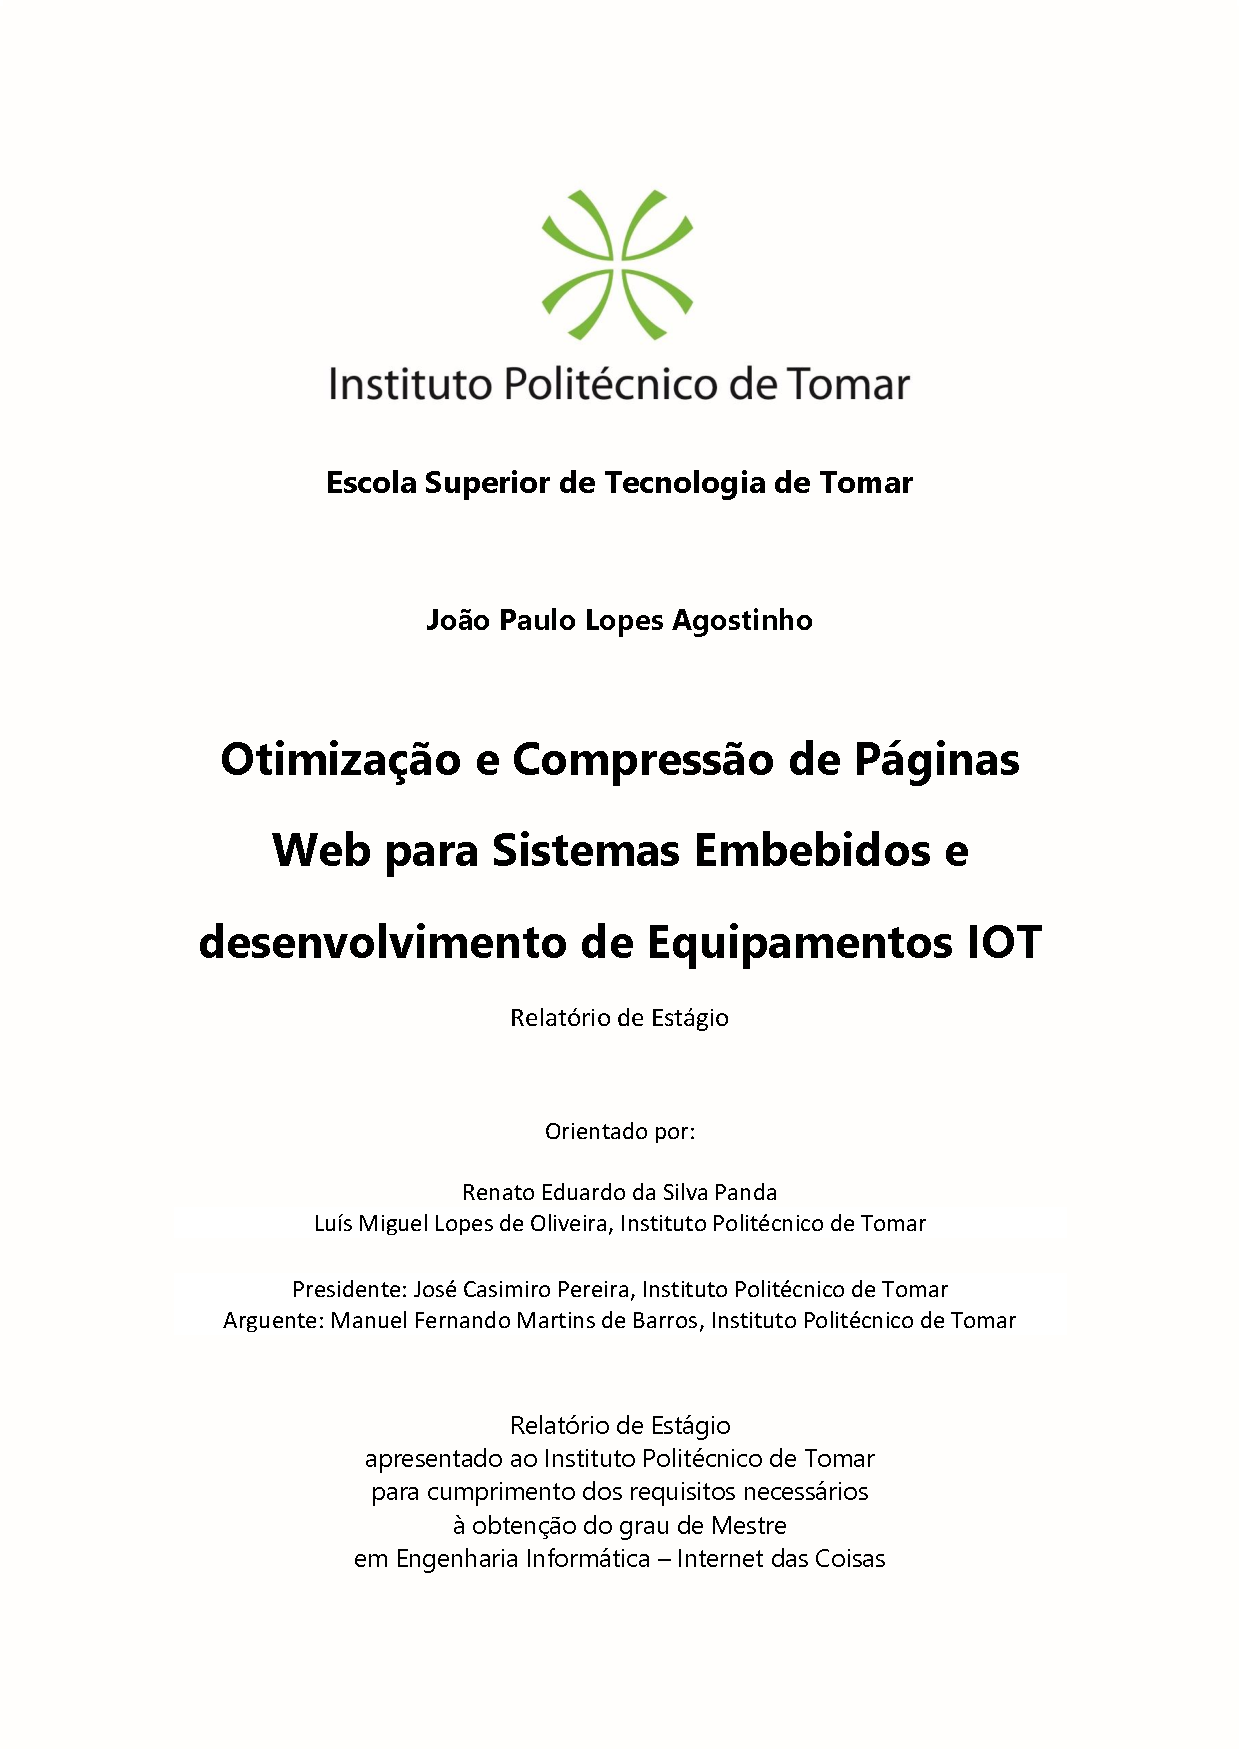
\includepdf[pages={-}]{images/cover/capa.pdf}
% Blank page
\newpage
\thispagestyle{empty}
\mbox{}
% Title page 1
%\begin{titlepage}
\thispagestyle{empty}

\begin{center}
% IPT Logo and Name

\includegraphics[width=0.8\textwidth]{images/logo_ipt.jpg}
% Thesis name
\vspace{1cm}
{\huge{\textbf{\thesistitle}}\par}
\vspace{1.5cm}
{{\large{Dissertação de Mestrado}}\par}

\vspace{1.5cm}
{\large{\textbf{Orientado por:}\\
Prof. Dr. Einstein \\
Prof. Dr. Marie Curie \\
Prof. Dr. Darth Vader
}}

\vspace{1cm}
{\large{\textbf{Juri:} \\
Prof. Dr. Steve Jobs \\
Prof. Dr. Bill Gates \\
Prof. Dr. Mark Zuckerberg
}}

% Final Stuff
\vfill
Dissertação apresentada ao Instituto Politécnico de Tomar para cumprimento dos requisitos necessários à obtenção do grau de Mestre em Engenharia Informática – Internet das Coisas

\vspace{0.5cm}
{\large \statedate\par}


\end{center}
\end{titlepage}  
% Blank page
%\newpage
%\thispagestyle{empty}
%\mbox{}

% Agradecimentos
\titleformat{\chapter}[display]{\rmfamily\Large\bfseries}{\thechapter}{0.5ex}{\centering}[\vspace{-0.5ex}\rule{\textwidth}{0.3pt}]
\chapter*{AGRADECIMENTOS}
\addcontentsline{toc}{chapter}{Agradecimentos}
\titleformat
{\chapter} % command
[display] % shape
{\bfseries\Large\itshape} % format
{Story No. \ \thechapter} % label
{0.5ex} % sep
{
    \rule{\textwidth}{1pt}
    \vspace{1ex}
    \centering
} % before-code
\par\par
Quero agradecer à minha família e amigos, pelo apoio dado nos bons e maus momentos não só durante a vida académica, mas durante toda a minha vida.\par
Aos meus colegas de curso e professores pelos bons tempos que foram passados nas aulas deste Mestrado.\par
Quero agradecer igualmente ao meu orientador, o professor Renato Panda por ser meu orientador e estar sempre disponível para ajudar nesta última fase do Mestrado.\par
À empresa Captemp pela possibilidade de realizar o estágio para conclusão de mais uma etapa da minha vida.\par

% You can add blank pages here, if you like
\newpage\null\thispagestyle{empty}\newpage

% RESUMO
\titleformat{\chapter}[display]{\rmfamily\Large\bfseries}{\thechapter}{0.5ex}{\centering}[\vspace{-0.5ex}\rule{\textwidth}{0.3pt}]
\chapter*{RESUMO}
\addcontentsline{toc}{chapter}{Resumo}
% Resumo em Português

\vspace{1cm}
\noindent
\par Este relatório de estágio foi realizado no âmbito do estágio inserido no Mestrado em Engenharia Informática-Internet das Coisas da Escola Superior de Tecnologia de Tomar do Instituto Politécnico de Tomar, e tem como objetivo colocar em ambiente real os conhecimentos adquiridos no percurso académico.

\par O estágio tem inerente 4 projetos associados à área do IOT e da monitorização de ambientes e/ou objetos com recurso a diversas soluções. O primeiro projeto, referente ao equipamento "Nidus" já existente. Este equipamento disponibilizado em vários modelos permite a ligação de vários tipos de sensores e atuadores  e centralizar o sistema de monitorização. Este equipamento é capaz igualemente a comunicação dos dados para um portal \textit{Cloud} onde é posível analizar os dados enviados pelos vários equipamentos. Neste projeto é necessário a análise do estado atual do projeto e dar continuidade ao suporte do \textit{Front-end} WEB do equipamento. Este projeto pretende estudar e alterar os métodos de desenvolvimento da página referentes á compressão dos ficheiros para reduzir o espaço ocupado pelas páginas WEB em equipamentos de baixos recursos computacionais e armazenamento, a adoção de um melhor método para utilização de imagens nas interfaces WEB em equipamentos com armazenamento limitado e o desenvolvimento de novas funcionalidades tais como um sistema de internacionalização de modo a disponibilizar o equipamento noutros idiomas, sempre tendo em, conta o baixo armazenamneto disponível. Os restantes projetos serão desenvolvidos de raiz durante o estágio  a pedido dos clientes, por soluções à medida, ou quer pela inovação e evolução dos produtos da empresa, e consistem em novos equipamentos para monitorização.

\par O segundo projeto é referente ao desenvolvimento de um equipamento IOT que tire partido das vantagens da nova tecnologia de comunicação o \textit{Narrowband} (NB-IOT). Neste equipamento irá ser possivel adicionar vários sensores já comercializados pela Captemp. O equipamento é capaz de realizar as leituras de todos os sensores connectados, realizar o armazenamento em Log para posterior envio para o portal \textit{Cloud} para consulta futura ou gestão da alarmística correspondente. Este equipamento é igualmente capaz de realizar uma configuração bi-direcional de modo a ser possível realizar a sua configuração através do portal \textit{Cloud}.

\par Paralelamente aos projetos anteriores e com o emergir de novas técnologias tais como os \textit{Beacons Bluetooth Low Energy} e pela sugestão de diversos clientes de uma nova solução de monitorização portátil e simples, foi criado o projeto "Kea Tracker" composto por \textit{Beacons} e uma aplicação \textit{Mobile} para \textit{Smartphones}, responsável por perioódicamente realizar a leitura dos sensores presentes nos \textit{Beacons}, o seu armazenamento e posterior envio para o portal \textit{Cloud}, à semelhança do projeto anterior. Neste projeto o \textit{Beacon} é igualmente capaz de registar em Log interno para caso exista falha de comunicação com a aplicação \textit{Mobile}, posteriormente esses dados serem descarregados quando o \textit{Smartphone} estiver disponível.

\par O último projeto referente deste estágio, foi solicitado pelo cliente que pretende uma plataforma WEB para localizar pessoas em ambientes \textit{indoor}. Esta solução baseia-se no desenvolvimento de uma solução composta por localizadores, \textit{Gateways} e uma plataforma WEB onde seja possível realizar o \textit{Tracking} de pessoas e de objetos em ambientes \textit{indoor} num mapa e assim gerir os tempos de acesso a zonas definidas, criar alertas, ou simplesmente gerir o stock dos armazéns. Este projeto, à semelhança do projeto "Kea Tracker", usa como tecnologia de suporte \textit{Beacons Bluetooth Low Energy} (BLE) para fazer o tracking em tempo real.




\bigskip

\textbf{Palavras chave:}
IOT, Monitorização, Compressão WEB,Compressão de Imagens,NB-IOT,Beacon,BLE, Indoor Tracking, Bluetooth Tracking

%\newpage\null\thispagestyle{empty}\newpage  %!!!!!!!!!!!!!!!!!!!!!!!!!!!!!!!!!!!!!!!!!!!!!!!!!!!!!!!!!!!!!!!!!!!!!!!!!!!!!!!!!!!!!!!!!!!!!!!!!!!!!!!!!!!!!!se for necessario

%ABSTRACT
\titleformat{\chapter}[display]{\rmfamily\Large\bfseries}{\thechapter}{0.5ex}{\centering}[\vspace{-0.5ex}\rule{\textwidth}{0.3pt}]
\chapter*{ABSTRACT}
\addcontentsline{toc}{chapter}{Abstract}
% Abstract in English

\vspace{1cm}
\noindent
\textbf{} 

\par This traineeship report was made in the scope of the traineeship inserted in the master's degree in Computer Engineering -Internet of Things at the School of Technology of Tomar from the Polytechnic Institute of Tomar, and has a goal place in real environment the knowledge acquired in the academic path.

\par The traineeship has inherent 4 associated projects at the area of IOT and the monitoring of environments and/or objects using different solutions. One of the projects, "Nidus" already existed and it is necessary to analyze the project to continue the support of Front-end. In this project, it is necessary to study and change the page development methods related to file compression to reduce the space occupied by the WEB pages, the adoption of a better method for using images on the WEB interfaces on equipment with low resources and the development of new features such as an internalization system in order to make the equipment available in other languages. The remaining projects will be developed from scratch during the traineeship, or by clients requesting custom solutions or by the innovation/evolution of the company's products, and consist of new equipments for monitoring, namely environmental monitoring and Tracking of objects.

\par The second project is relative of the development of an IOT device that takes advantage of the new communication technology NB-IOT. In this equipment it is possible to add several sensors, and the equipment is able to perform the readings of the various sensors, storage in Log for later upload to a Cloud portal for future preview or make alerts.
\par In parallel with the previous project and with the emergence of new technologies such as Bluetooth Low Energy Beacons and the request by several customers for a new portable and simple monitoring solution, the "Kea Tracker" project was created, composed with several Beacons and an application Mobile responsible for reading the sensors present in Beacons and upload them to the Cloud portal. In this project, Beacon must also have an internal Log system for communication failure with the Mobile application.
\par The last project of the traineeship, requested by the client, is based on the development of a solution composed of Sensors and Gateways and a WEB platform that makes it possible to Tracking people and objects in indoor environments and thus manage access times, create alerts, or simply manage the stock of warehouses. This project uses as support technology Bluetooth Low Energy Beacons (BLE) to do real-time tracking.

\bigskip

\textbf{Key words:} 
IOT, Monitoring, WEB Compression, Image Compression, NB-IOT, Beacon, BLE, Indoor Tracking, Bluetooth Tracking
% And here as well

\clearpage \cleardoublepage


% INSPIRATIONAL QUOTE
% Setup
\setlength\epigraphwidth{12cm}
\setlength\epigraphrule{0pt}
\makeatletter
\patchcmd{\epigraph}{\@epitext{#1}}{\itshape\@epitext{#1}}{}{}
\makeatother
% Actual Quote
\vspace*{\fill}
\epigraph{"Persistence is the shortest path to success"}{}
{ ---  \textup{Charles Chaplin}}
\vspace*{\fill}

\clearpage \cleardoublepage

%\newpage\null\thispagestyle{empty}\newpage  %!!!!!!!!!!!!!!!!!!!!!!!!!!!!!!!!!!!!!!!!!!!!!!!!!!!!!!!!!!!!!!!!!!!!!!!!!!!!!!!!!!!!!!!!!!!!!!!!!!!!!!!!!!!!!!se for necessario



% TABLE OF CONTENTS

\titleformat{\chapter}[display]{\rmfamily\Large\bfseries}{\thechapter}{0.5ex}{\centering}[\vspace{-0.5ex}\rule{\textwidth}{0.3pt}]
\tableofcontents
\clearpage

\newpage\null\thispagestyle{empty}\newpage %!!!!!!!!!!!!!!!!!!!!!!!!!!!!!!!!!!!!!!!!!!!!!!!!!!!!!!!!!!!!!!!!!!!!!!!!!!!!!!!!!!!!!!!!!!!!!!!!!!

\addcontentsline{toc}{chapter}{Índice de Figuras}
\listoffigures
\clearpage %\cleardoublepage %for openright
\addcontentsline{toc}{chapter}{Índice de Tabelas}
\listoftables

\newpage\null\thispagestyle{empty}\newpage %!!!!!!!!!!!!!!!!!!!!!!!!!!!!!!!!!!!!!!!!!!!!!!!!!!!!!!!!!!!!!!!!!!!!!!!!!!!!!!!!!!!!!!!!!!!!!!!!!!

\clearpage %\cleardoublepage %for openright
\renewcommand\lstlistlistingname{ÍNDICE DE ALGORITMOS}
\addcontentsline{toc}{chapter}{Índice de Algoritmos}
\lstlistoflistings
\renewcommand\lstlistingname{Algoritmo}
\renewcommand\lstlistlistingname{Algoritmos}

\newpage\null\thispagestyle{empty}\newpage %!!!!!!!!!!!!!!!!!!!!!!!!!!!!!!!!!!!!!!!!!!!!!!!!!!!!!!!!!!!!!!!!!!!!!!!!!!!!!!!!!!!!!!!!!!!!!!!!!!

%\clearpage \cleardoublepage %for openright
\addcontentsline{toc}{chapter}{Acrónimos}
% LIST OF ACRONYMS
\chapter*{ACRÓNIMOS}
\addcontentsline{toc}{chapter}{Acrónimos}

\begin{acronym}[list\_acronyms]

%\newacronym{BLE}{BLE}{Bluetooth Low Energy}
%\newacronym{GSM}{GSM}{Global System for Mobile Communications}
%\newacronym{JPG}{JPG}{Joint Photographic Group}
%\newacronym{HTML}{HTML}{HyperText Markup Language
%\newacronym{NB-IOT}{NB-IOT}{Narrowband IoT}
%\newacronym{PNG}{PNG}{Portable Network Graphics}
%\newacronym{RTC}{RTC}{Real Time Clock}
%\newacronym{SVG}{SVG}{Scalable Vector Graphics}


%\printglossary[type=\acronymtype]
\end{acronym}
%\clearpage \cleardoublepage %for openright
% BODY
%\newpage !!!!!!!!!!!!!!!!!!!!!!!!!!!!!!!!!!!!!!!!!!!!!!!!!!!!!!!!!!!!!!!!!!!!!!!!!!!!!!!!!!!!!!!!!!!!!!!!!!!!!!!!
\thispagestyle{empty}
\mbox{}

\fancyhead[LE,RE]{\slshape\rightmark}
\fancyhead[LO,RO]{\slshape\leftmark}
\fancyhead[RE,LO]{}
\pagestyle{fancy}
\titleformat{\chapter}[display]
    {\normalfont\huge\bfseries}{\chaptertitlename\ \thechapter}{20pt}{\Huge}
\titlespacing*{\chapter}{0pt}{0pt}{20pt}

\chapter{Introdução}
\pagenumbering{arabic}
\section{Contextualização}
\par
Atualmente a sociedade vive rodeada de tecnologias indispensáveis e de ambientes que se intitulam inteligentes (\textit{smart}), mas nem sempre foi assim.\par
Desde cedo, mesmo antes de existir tecnologia, o homem tendeu a procurar e encontrar coisas que melhorassem a sua vida e bem-estar pessoal e da sociedade, mas para chegar a humanidade está hoje é necessário recuar na história algum tempo para marcos importantes da tecnologia.\par
Um dos marcos muito importantes para o desenvolvimento dos sistemas embebidos e de sistemas de monotorização foi a invenção dos processadores. Com o surgimento dos processadores começaram a surgir os primeiros sistemas embebidos e sistemas de monotorização. Com o passar dos anos até aos dias de hoje a tecnologia tem vindo a evoluir e por consequência os sistemas também se adaptaram para os padrões de atualmente.\par
Uma das partes mais importantes num sistema embebido é a sua interface disponível para o utilizador, as principais e mais usadas nos dias de hoje são a linha de comandos e a WEB, comuns para configurações á distância e as interfaces dos próprios equipamentos como os ecrãs com \textit{software} proprietário.

\section{A Empresa}
\par
A empresa CapTemp, Lda localizada em Pombal, Leiria é uma empresa, focada em desenvolvimento de soluções de monitorização, controlo, supervisão e de soluções à medida consoante os requisitos do cliente. Para criar um sistema de monitorização é necessário o sistema possuir sensores, atuadores, coletores de dados e software para analisar os dados provenientes dos sensores de modo a possuir capacidade de atuar com base nesses valores. A Captemp é responsável pelo desenvolvimento de todos estes componentes passando pelos sensores até ao \textit{software} responsável por analisar e armazenar os dados.\par
Uma das subáreas da empresa é a disponibilização de um registador de temperatura e respetivo \textit{software} certificado para Meteorologia Legal. A Meteorologia Legal é aplicada a todas as câmaras com uma volumetria superior a 10 metros cúbicos, onde a regulamentação indica que tem de existir um sistema certificado para o registo das temperaturas.
Faz parte deste conjunto o \textit{Software} “CapTemp SQL”, representado na figura \ref{figcaptempsql}, responsável por guardar os dados provenientes dos sensores ligados ao registador.\par
\begin{figure}[ht]
  \centering
  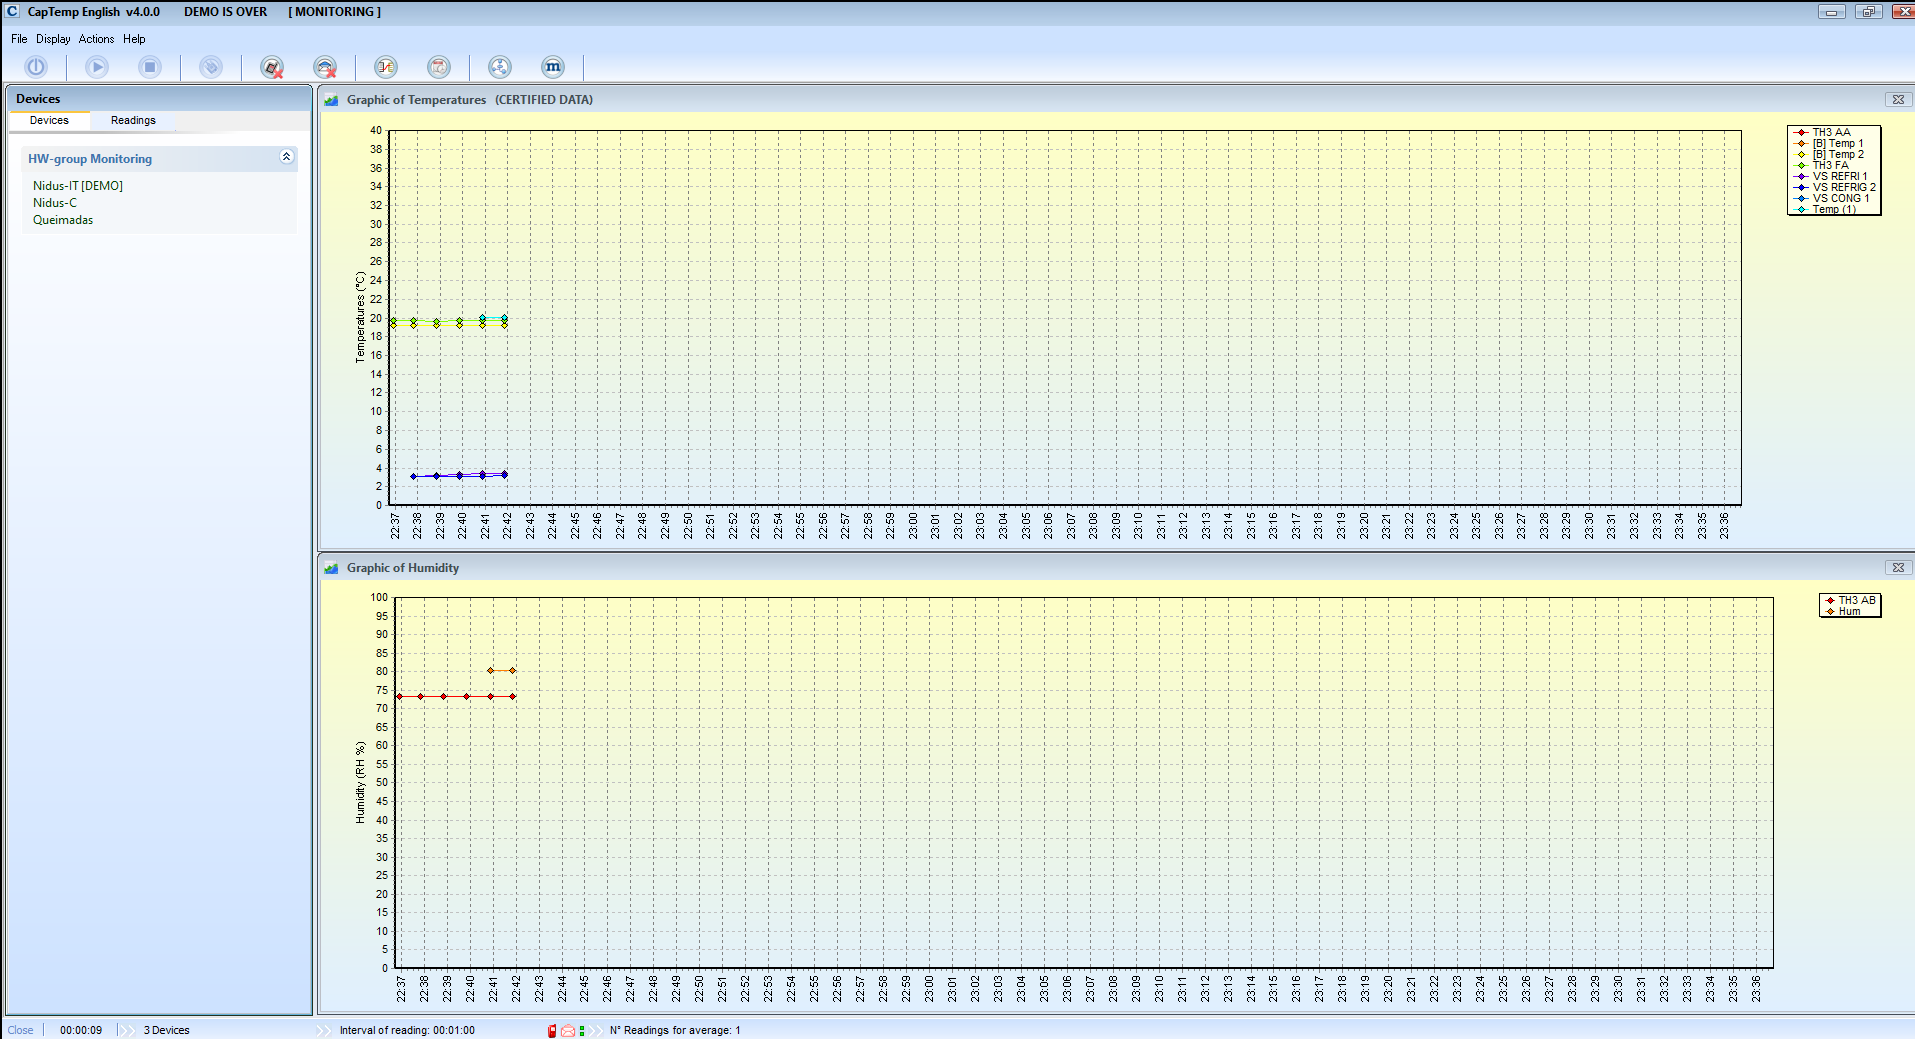
\includegraphics[width=1.00\textwidth]{images/captemp.png}
  \caption{CapTemp SQL}\label{figcaptempsql}
\end{figure}
O registador desenvolvido pela Captemp, representado na figura \ref{fignidusCl} denomina-se por Nidus-C, um registador que suporta até 32 sensores.\par

\begin{figure}[ht]
  \centering
  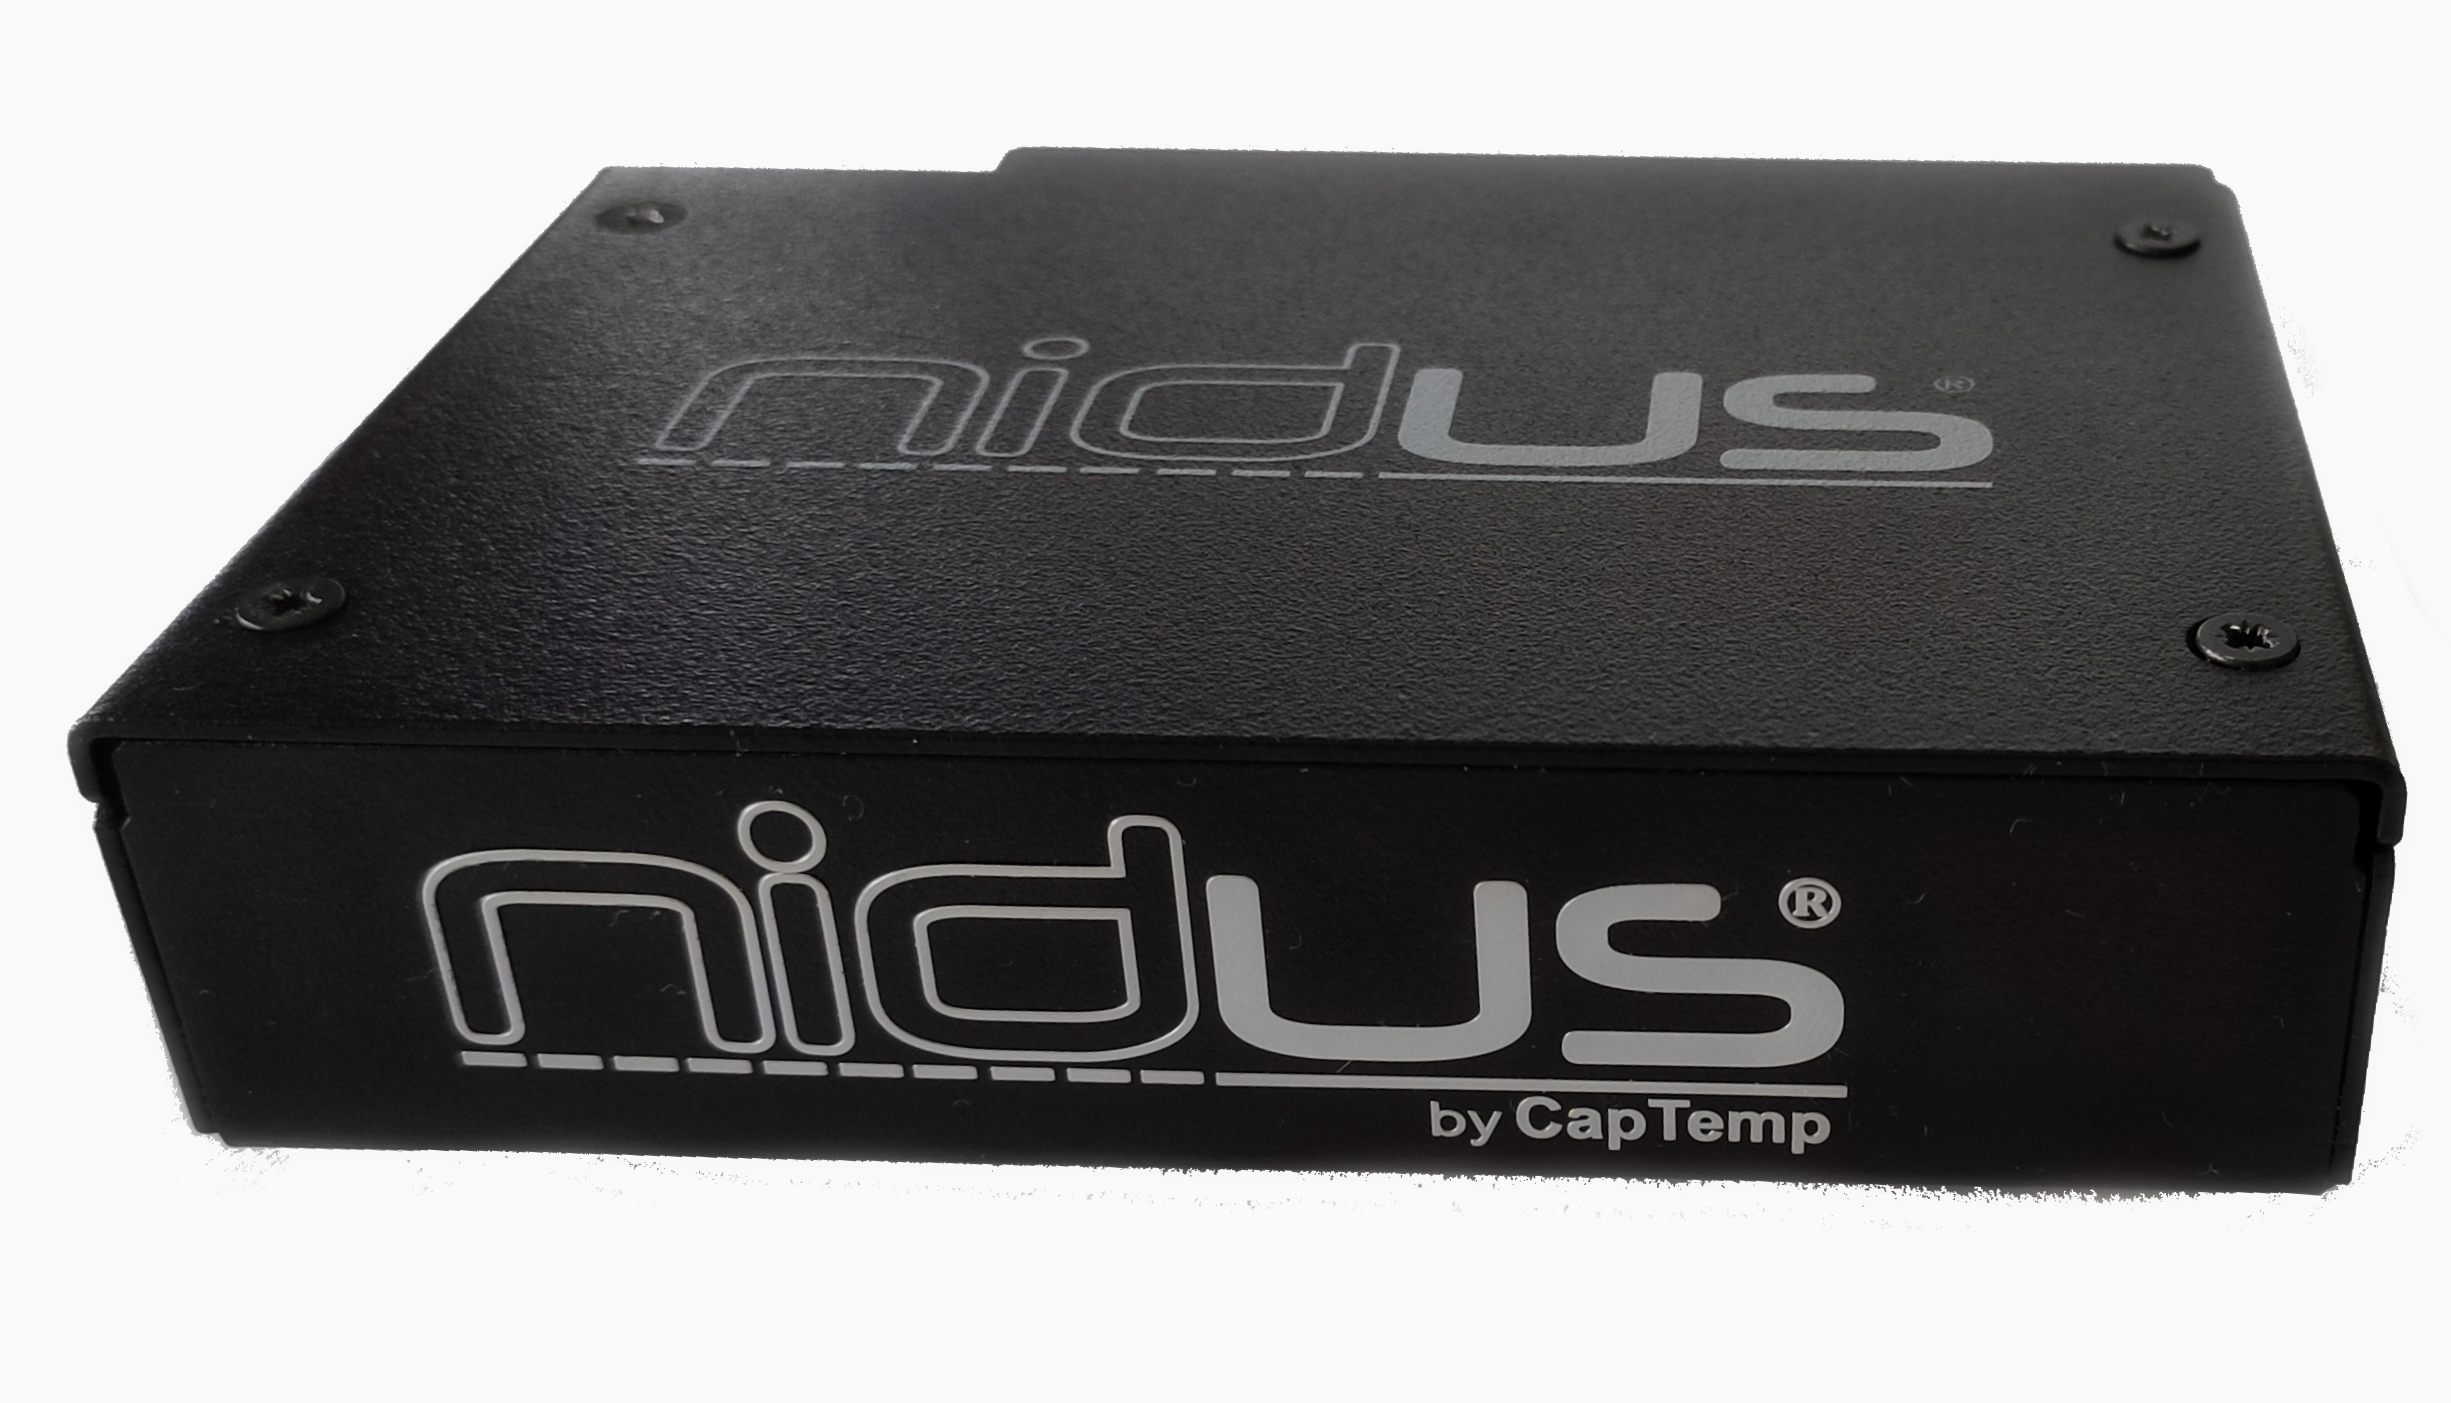
\includegraphics[width=0.45\textwidth]{images/nidus.jpg}
  \caption{Coletor de dados Nidus-C}\label{fignidusCl}
\end{figure}

Com a necessidade de mais funcionalidades, a Captemp criou diversas variantes da Nidus-C, representadas na Figura \ref{fignidusall} para aplicar em outras áreas para além da Meteorologia Legal. Das quais surgiram a Nidus-C+, uma versão similar da Nidus-C acrescentando a possibilidade de adicionar sensores \textit{Wireless}. A Nidus-IT e Nidus-IT+ duas versões com as funcionalidades da Nidus-C e Nidus-C+ respetivamente, acrescentando Inputs e Outputs ao sistema de monitorização. Para soluções exclusivamente \textit{Wireless} nasce a Nidus-W suportando apenas sensores Wireless. Por último é desenvolvido a Nidus-R, baseada na Nidus-IT especialmente desenhada a pensar em ambientes IT com suporte para montagem em bastidores.
\par
\begin{figure}[ht]
  \centering
  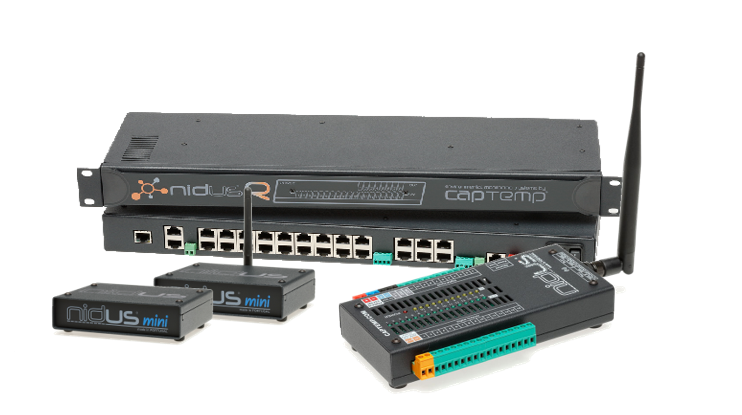
\includegraphics[width=0.65\textwidth]{images/nidusall.png}
  \caption{Universo Nidus}\label{fignidusall}
\end{figure}

No setor dos sensores foi desenvolvido o TH3, um conversor RS485 permitindo às diversas Nidus, ligar por RS485 a sensores 1Wire além dos dois inputs possuídos no TH3. Nos sensores \textit{Wireless}, foi desenvolvido o Airo à semelhança do TH3 possui dois inputs, um ecrã e possibilita a ligação de sensores 1Wire. Permite ainda a leitura de todos os Airo adicionados na Nidus ao mesmo tempo, tecnologia desenvolvida pela Captemp denominada por Captemp AST \cite{Captemp_AST}. Ambos os sensores estão representados na Figura \ref{figairoth3} 
\begin{figure}[ht]
  \centering
  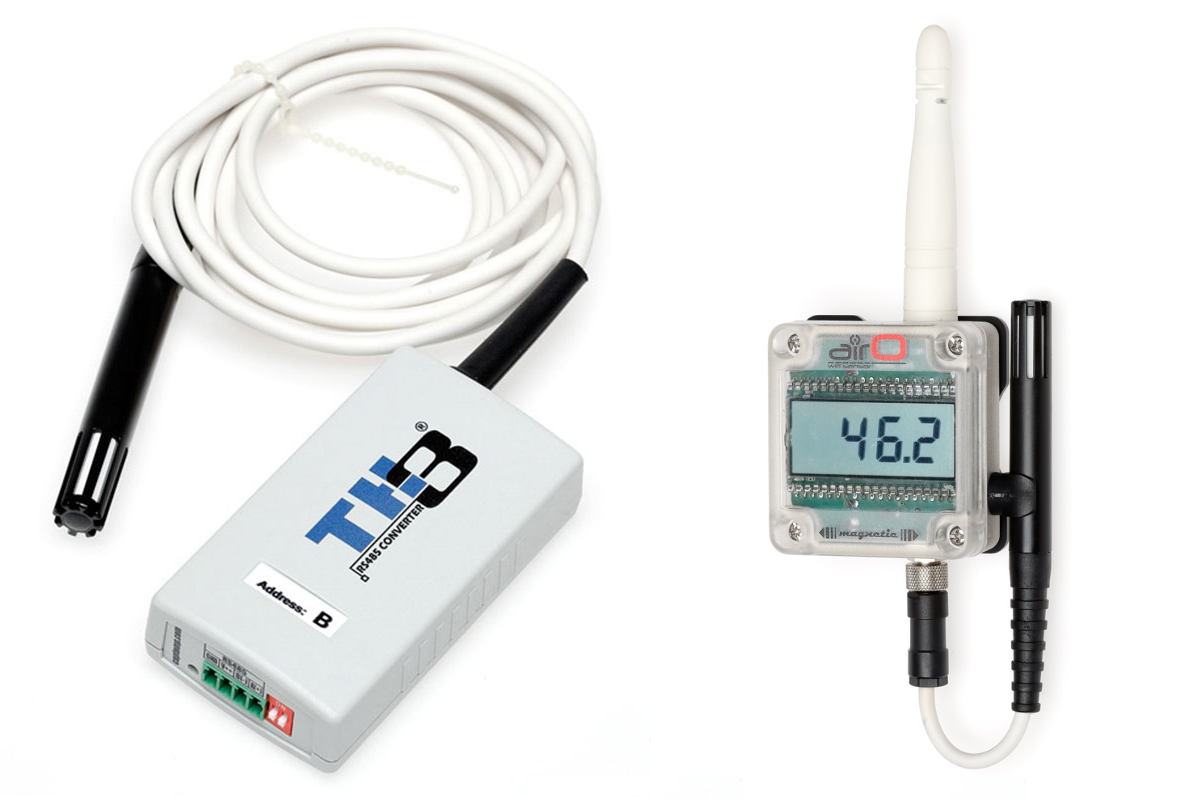
\includegraphics[width=0.45\textwidth]{images/th3airo.png}
  \caption{ TH3 e Airo}\label{figairoth3}
\end{figure}
\par
Em desenvolvimento encontram-se sensores com recurso a tecnologias NB-Iot, Beacon's BLE e Lora entre outras soluções tais como sistemas de rastreamento de Febre em tempo real com recurso a inteligência artificial.
\par
A Captemp desenvolve igualmente um portal \textit{Cloud} denominado Senslive (Figura \ref{figsenslive}) que possibilita a centralização dos sistemas de monitorização numa única plataforma \textit{Cloud}.

\begin{figure}[ht]
  \centering
  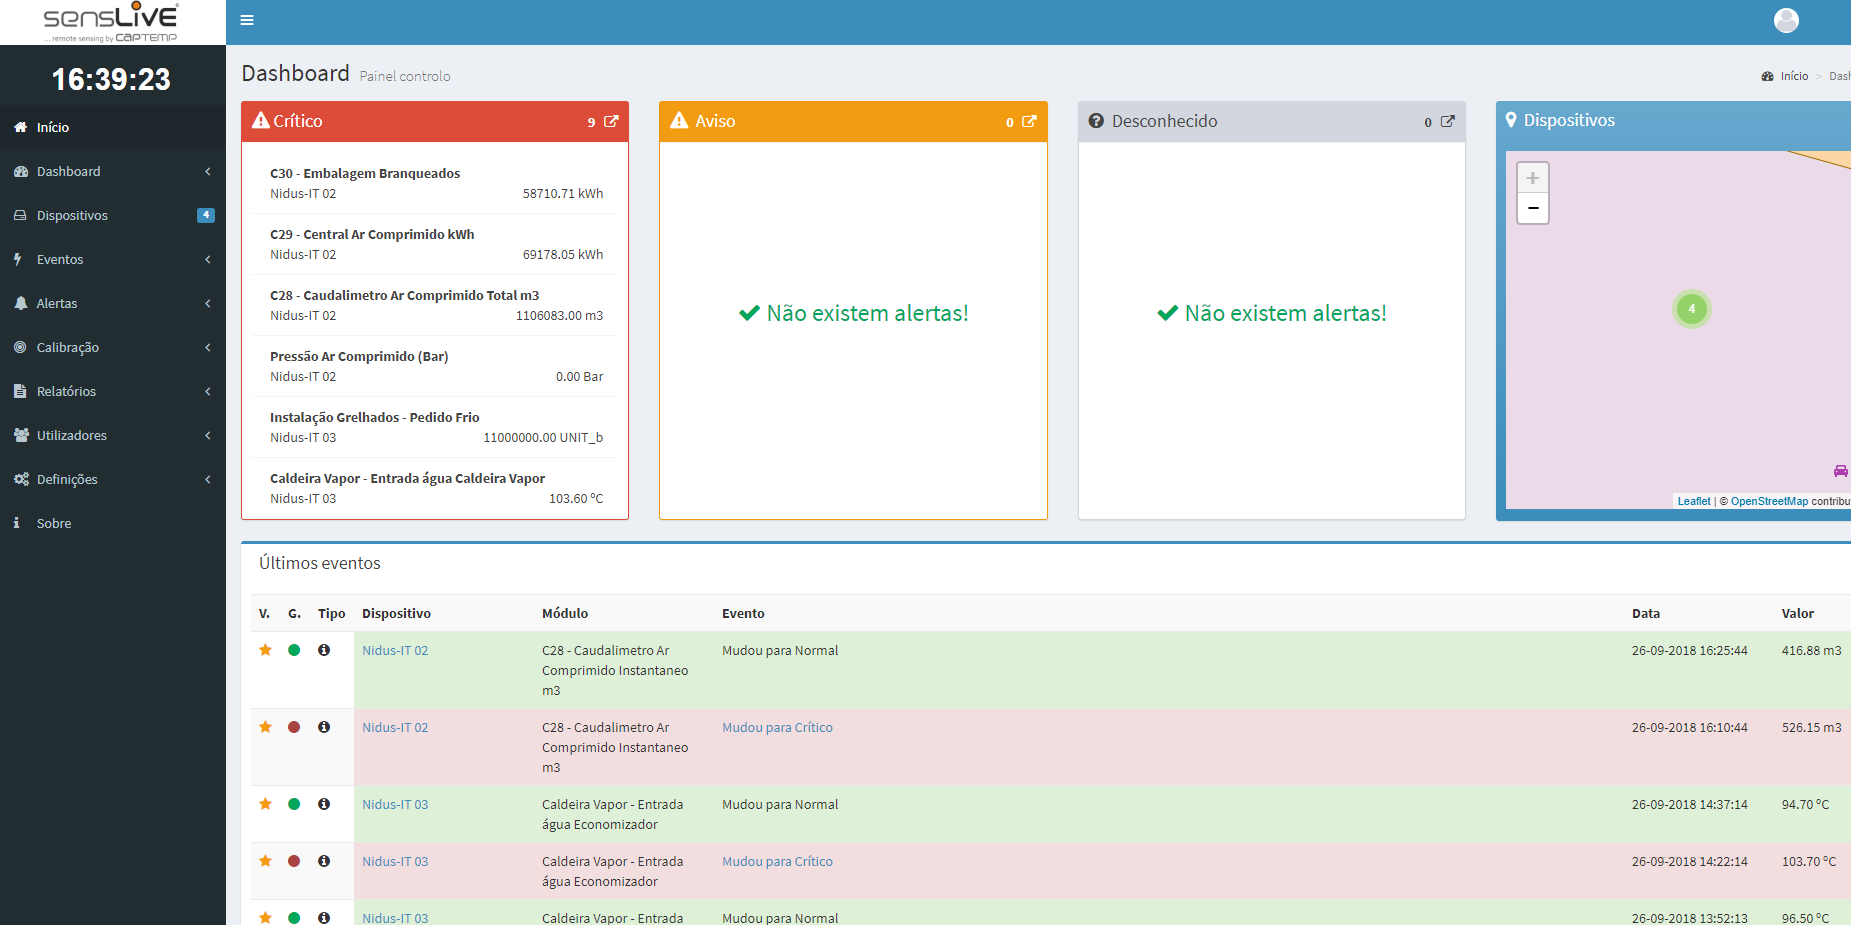
\includegraphics[width=0.95\textwidth]{images/mwsnap0791.png}
  \caption{ Portal Senslive}\label{figsenslive}
\end{figure}



\section{Motivação e Objetivos}
\par
O estágio é uma forma do estudante colocar numa situação de contexto profissional os conceitos adquiridos em contexto académico. A realização de um estágio é também uma mais valia pois possibilita o adquirir de experiência profissional que não é possível obter em contexto escolar.
\par
A Captemp com os projetos a desenvolver pretende melhorar constantemente os seus equipamentos e as suas interfaces, por questões de \textit{Markting} quer pelo próprio evoluir da tecnologia e necessidade de novas funcionalidades e o seu desenvolvimento requer o alojamento de mais recursos como por exemplo a memória ou disco, estes limitados nestes tipos de equipamentos e onde é preciso fazer uma correta escolha de soluções e de implementação. 
\par
Ao longo do estágio, o objetivo será estudar variados mecanismos que permitam adotar recursos web modernos nos equipamentos de baixos recursos. Serão aplicados vários conhecimentos adquiridos durante o percurso académico de modo a melhorar a interface para o utilizador, técnicas de otimização de código, compressão de ficheiros, manipulação de imagens de modo a ocupar o mínimo de espaço permitindo futuros desenvolvimento e melhorias, dando continuidade ao suporte do projeto Nidus. Igualmente serão criados três novos projetos de desenvolvimento de novos equipamentos e soluções que tiram partido de novas tecnologias como o NB-Iot e Beacon’s BLE onde é necessário devido á escassez de recursos fazer a correta gestão dos mesmos e a implementação de variados algoritmos.
\par
Nas seguintes secções são apresentadas uma breve descrição de cada projeto, dos equipamentos já existente e desenvolvido, e as funcionalidades a desenvolver em cada projeto.
\subsection{Nidus}
\par
O projeto "Nidus" tem como objetivo dar suporte ao \textit{Front-end} das Nidus já existentes para correções de bugs encontrados em versões anteriores, otimização de código, de modo a ocupar o mínimo espaço, possibilitando deixar memória livre para desenvolvimentos futuros, desenvolver versões customizadas com \textit{layouts} a pedido do cliente com funcionalidades especificas, ou simplesmente melhorar a página seguindo a tendência de equipamentos concorrentes.
\subsection{NB-Iot}
Com o surgimento da nova tecnologia NB-Iot surgiu a necessidade de serem criados equipamentos que tirem partido dessa tecnologia e as suas vantagens. Para tal durante o estágio será desenvolvido um dos equipamentos que tira partido da tecnologia. Este projeto tem como por objetivo criar uma versão de raiz, simplificada e mais barata de um outro equipamento de NB-Iot em desenvolvimento pela Captemp, através do módulo Xbee da DIGI e da sua programação em Micropython. Durante o projeto será necessário garantir a correta gestão de memória, gestão de Logs internos, comunicação com os sensores físicos, comunicação bidirecional e encriptação com o portal Senslive.
\subsection{Kea Tracker}
O "Kea Tracker" é um projeto de Beacon’s BLE que comunicam com o \textit{smartphone}, onde é possível definir alertas locais no \textit{smartphone} e envio dos dados obtidos dos sensores das beacon’s e envio para a plataforma Senslive.
Tal como o projeto anterior será necessário além de criar uma aplicação para \textit{smartphone}, criar \textit{Firmware} específico para as beacon’s que na ausência de comunicação com o \textit{smartphone} devem armazenar em Log as leituras dos sensores e quando este está ao alcance descarregar para o \textit{smartphone}.
\subsection{dot.Tracker}
A pedido de um cliente foi solicitado o desenvolvimento de uma plataforma para localização de pessoas e objetos em ambientes \textit{inndoor}. O cliente pretende ter uma plataforma onde seja capaz de ver em tempo real a posição de pessoas e objetos definidos previamente, definir zonas de alerta, e consultar o histórico de movimentos. Neste projeto irão ser usadas beacon's BLE e vários \textit{Gateways} BLE estrategicamente colocados no edifício e responsáveis por receber o \textit{broadcast} das beacons que por sua vez transmitem para o servidor através da rede informática do cliente do serviço. O projeto é constituído pelo desenvolvimento da plataforma de gestão e visualização, pelo recetor dos pacotes provenientes dos equipamentos e respetivos cálculos segundo o algoritmo a adotar.

\section{Problemas identificados}
Foram identificados diversos problemas em cada um dos projetos a desenvolver durante o estágio. Uma breve descrição é apresentada de seguida.
\par
A página WEB da Nidus desde a sua criação já sofreu muitas alterações para seguir os padrões e tendências da concorrência e, portanto, está em constante atualização. Atualmente com a mundialização quase todas as pessoas sabem inglês, mas existem algumas pessoas que ou não sabem ou preferem usar a língua nativa. Para tal a Captemp pretende desenvolver uma página WEB com um sistema de tradução e diversas línguas que seja possível de alojar na memória do equipamento, devido aos problemas já referidos para o utilizador escolher a linguagem e assim cativar mais clientes e expandir a Captemp para outros países. Com o acréscimo do serviço de internalização surge o problema de uma interface com necessidade de mais armazenamento. Terão de ser estudadas otimizações que se possam implementar no código já existente. Existe a necessidade de estudar o melhor método de compressão da página mantendo o GZIP utilizado atualmente ou migrar para outro mais recente como o Brotli e a compressão de imagens migrando as imagens existentes para imagens SVG, possibilitando outras soluções para a página com sistemas mais interativos e ocupando o menor espaço disponível. Além dos problemas referidos anteriormente poderão surgir novas funcionalidades, a pedido de clientes, como por exemplo páginas com layout específicos ou novos sensores e a simples correção de possíveis Bugs encontrados.
\par
Outro problema a resolver detetado pelo \textit{feedback} recebido dos clientes é a complexidade para a criação de eventos, ações e reações, que controlam o Sistema Nidus. Para isso a Captemp pretende reformular a estrutura de gestão de eventos para um sistema mais visual e atual similar ao Scratch, um \textit{software} utilizado atualmente para ensinar a crianças as bases da programação e elas mesmos criarem alguns programas sem saber nenhuma linguagem de programação. Na figura \ref{scratch} é apresentado um exemplo de programação usando a ferramenta Scratch, onde o utilizador com um sistema de blocos pode criar condições e eventos a despoletar consoante algumas condições.

\begin{figure}[ht]
  \centering
  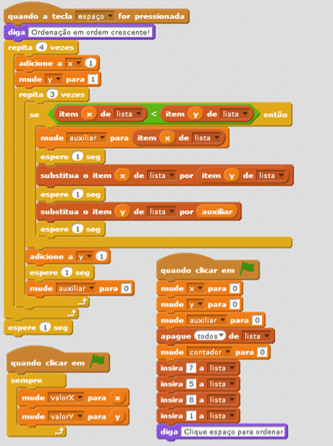
\includegraphics[width=0.50\textwidth]{images/scratch.png}
  \caption{ Programação com a ferramenta Scratch}\label{scratch}
\end{figure}

\par Outros problemas existentes, a resolver durante o estágio, são a criação de sistemas \textit{low-cost}, de outros equipamentos CapTemp, para clientes que não necessitem de tantas funcionalidades com a introdução da alternativa para NB-Iot com recurso ao módulo Xbee da Digi, e a substituição de produtos antigos descontinuados, os data-logger(Figura \ref{ds1921}) e sua substituição por similares com as mesmas funções e mais tipos de sensores disponíveis, uma necessidade também já requisitada pelos clientes que pretendem monitorizar mais grandezas além da temperatura, mas com os padrões e tecnologias dos dias de hoje e com suporte para o novo Portal da Captemp o Senslive. Ou simplesmente o desenvolvimento de novos produtos a pedido dos clientes.

\begin{figure}[htb]
  \centering
  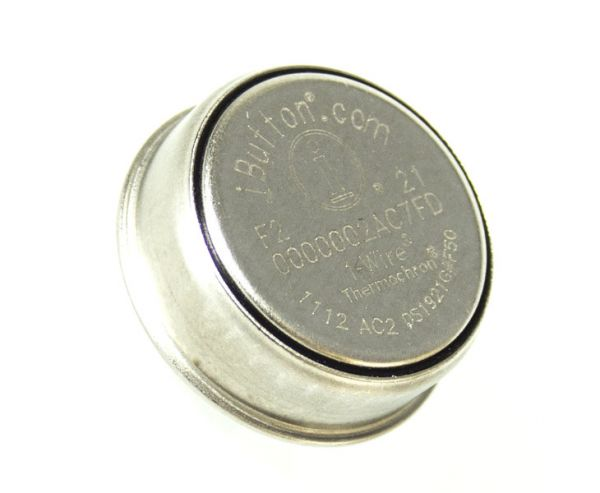
\includegraphics[width=0.20\textwidth]{images/ds1921.jpg}
  \caption{Data Logger iButton}\label{ds1921}
\end{figure}


\par
Em resumo os problemas a solucionar durante o estágio podem ser encontrados na seguinte lista:
\begin{itemize}
\item Melhorar a compressão da página WEB da Nidus;
\item Melhorar a compressão das imagens presentes na página WEB da Nidus;
\item Correção de Bugs da página Web da Nidus;
\item Melhorar o processo de criação de eventos;
\item Criação de uma página com sistema de tradução automático;
\item Versões customizadas da página WEB a pedido do cliente;
\item Seguir as tendências da concorrência;
\item Criação de soluções/equipamentos de baixo custo;
\item Substituição de produtos descontinuados;
\item Desenvolvimento de produtos à medida do cliente.

\end{itemize}

\section{Organização do relatório}

\par Este presente relatório está dividido em 5 capítulos. O primeiro capítulo faz a introdução ao tema e é apresentado os objetivos, o enquadramento do estágio e alguns aspetos inicias a considerar. 
\par No capítulo seguinte é apresentada a tecnologia e hardware pesquisado com fim a dar suporte a este mesmo estágio e uma pequena pesquisa sobre projetos/produtos similares quer na finalidade quer nas tecnologias usadas e o estado atual de cada projeto. 
\par O capítulo 3 apresenta o trabalho desenvolvido durante o estágio na empresa para a resolução dos problemas identificados. Este capítulo apresenta os detalhes técnicos das soluções escolhidas. 
\par No capítulo 4 são descritos os resultados dos testes efetuados às soluções propostas e desenvolvidas no capítulo 3.
\par Por fim no capítulo 5 é apresentada uma breve conclusão de todo o trabalho, dificuldades e algumas sugestões para futuras implementações. 


	% Arabic numbering starts

% For each chapter, you should have a bit of code that looks like this:
% \label allows you to later \ref that chapter.
% \input includes a different .tex file, so that you can have you dissertation
% neatly partitioned into several files. I recommend one file per chapter.
\chapter{Estado da Arte}
\label{chap:state_of_the_art}

\section{Introdução}
Nesta secção é apresentada o estado da arte dos projetos realizados durante o estágio na empresa CapTemp. Nessa ordem é apresentado o funcionamento do sistema do Nidus desenvolvido pela empresa CapTemp e a sua página de configuração e visualização. Na secção \ref{Página do Coletor de Dados Nidus} são apresentadas também as metodologias e tecnologias que o sistema implementa atualmente para a compressão das páginas que dão suporte ao sistema. Na secção \ref{nbiot}, \ref{kea} e  \ref{dot} irá ser introduzido o plano inicial dos projetos a desenvolver e a base já existente tal como as tecnologias que estes irão utilizar. Na secção \ref{solucoesDisponiveis} será abordado as soluções e tecnologias existentes na comunidade científica e alguns produtos similares, já existentes para os projetos anteriormente referidos.

\section{Coletor de Dados - Nidus} \label{Coletor de Dados - Nidus}
\par
O sistema Nidus, apesar das suas diversas versões de hardware partilha entre todas as versões o mesmo centro de processamento o módulo RCM6760 da Rabbit. O sistema Nidus é composto por dois módulos principais, o Back-end que gere toda a parte de leitura de sensores, de atuação e envio de alertas, log entre as demais funcionalidades e o Front-end, duas páginas WEB Single-Application de modo a não sobrecarregar o módulo com a interface e mover o processamento da interface para o browser do cliente. Na primeira página é possível visualizar os valores obtidos pelo Back-end com atualização em tempo real. Na segunda página e possível carregar as configurações para realizar alterações nas mesmas. A comunicação entre os dois componentes é feita através de XML. Para consultar os valores na primeira página o Front-end acede ao ficheiro values.xml gerado pelo Back-end onde contém todas os valores necessários. Na página de configurações á semelhança da primeira página os valores são carregados por um ficheiro XML o ficheiro setup.xml, incluindo a particularidade de aceitar pedidos POST de modo a alterar as configurações do equipamento.
\par A Nidus dispõe de base para o utilizador variadas funcionalidades tais como, leitura de sensores TH3 e Airo, INPUTS digitais, OUTPUTS digitais e analógico, leitura de sensores SNMP e MODBUS, envio de alertas via GSM e E-mail, programação de eventos, envio automático para um portal Cloud e Log Interno. Outras funcionalidades estão disponíveis mediante o pedido do cliente tais como sensores específicos, leitura de sensores por RS232 ou protocolos de comunicação específicos.
Na tabela \ref{tab0} são apresentadas as principais características do módulo RCM6760 da Rabbit.




\begin{table}[htb]
\centering
\caption{Especificações do Módulo RCM6760}\label{tab0}
\begin{tabular}{|c|c|}\hline
Microprocessor&Rabbit 6000 \\\hline
Frequencia do Microprocessor &200 MHz\\\hline
Flash Memory &4 MB (Código e Sistema de Ficheiros)\\\hline
SRAM&1 MB\\\hline
Power &260 mA 3.3V - Ethernet ON\\\hline
\end{tabular} 
\end{table}

\subsection{Páginas do Coletor de Dados Nidus} \label{Página do Coletor de Dados Nidus}
\par
O código desenvolvido de modo a chegar á fase de produção é comprimido e compilado de modo a que ocupe o mínimo espaço e possa ser armazenado na memória do módulo e coabitar com o Firmware de Back-end, segue os seguintes passos de desenvolvimento:
\begin{enumerate}
\item Desenvolvimento/ alteração do código JavaScript necessário; 
\item Compressão das Imagens necessárias com recurso a ferramentas online tais como o TinyPNG\cite{tinypng} e posterior conversão em Base64 para incluir no JavaScript a imagem e o mesmo poder fazer a gestão da apresentação
\item Compilação/compressão do JavaScript num ficheiro único com recurso ao Google Clousure Platform, nesta etapa para cada versão de hardware é compilado consoante os ficheiros a incluir, poupando o espaço não necessário como o código referente aos Inputs e Outputs na Nidus C, C+ e W, ou o código referente ao módulo wireless nas versões não Wireless.
\item Geração do minificado do código HTML
\item Compressão de cada ficheiro para o seu respetivo GZIP
\end{enumerate}
\par
Após estes passos fica disponível uma nova versão da página pronta a ser carregada na Nidus.
Na imagem \ref{fignidusPage} é apresentado o estado e layout de uma página da Nidus IT no momento do início do estágio.

\begin{figure}[ht]
\centering
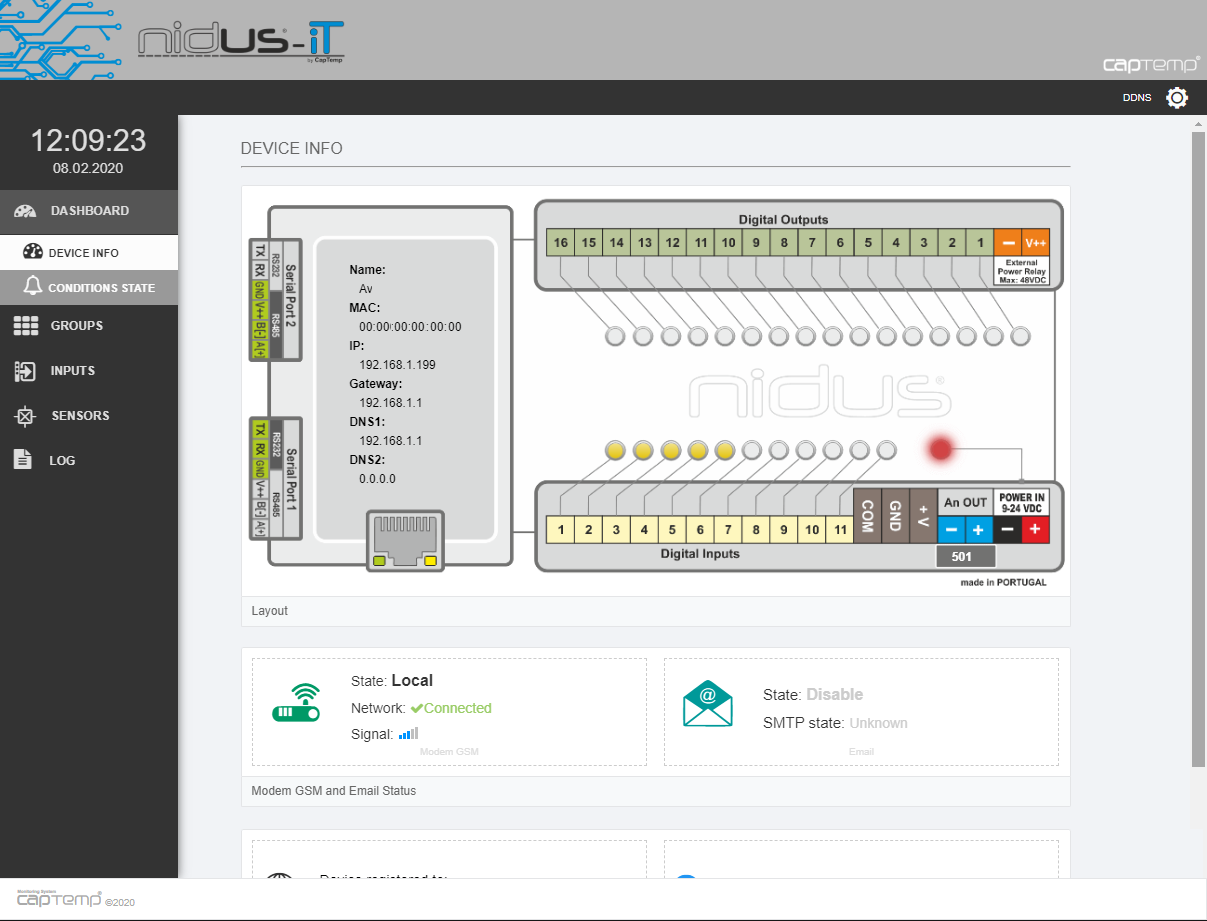
\includegraphics[width=0.75\textwidth]{images/layoutPAginaInit.png}
\caption{Layout página da Nidus IT no início do estágio}\label{fignidusPage}
\end{figure}


\section {NB-Iot \& Digi Xbee 3 }\label{nbiot}
\par
Os módulos Xbee 3 representado na figura \ref{figxbee} da DIGI dispõe recentemente de uma versão NB-Iot/ LTE. Ideal para projetos com baixo volume de transmissão de dados e com baixo consumo de energia. O módulo inclui também um compilador de Micropython, contundo a versão Micropython desenvolvida pela DIGI e incluída no módulo XBee, não inclui todas as funcionalidades do Micropyhton tais como por exemplo a biblioteca de gestão de Arrays e o módulo de "\_thread" pois o mesmo não tem suporte para multithread.
Na tabela \ref{tab1} são apresentadas as principais características do módulo XBee 3 da Digi\cite{Digixbee}.

\begin{figure}[ht]
\centering
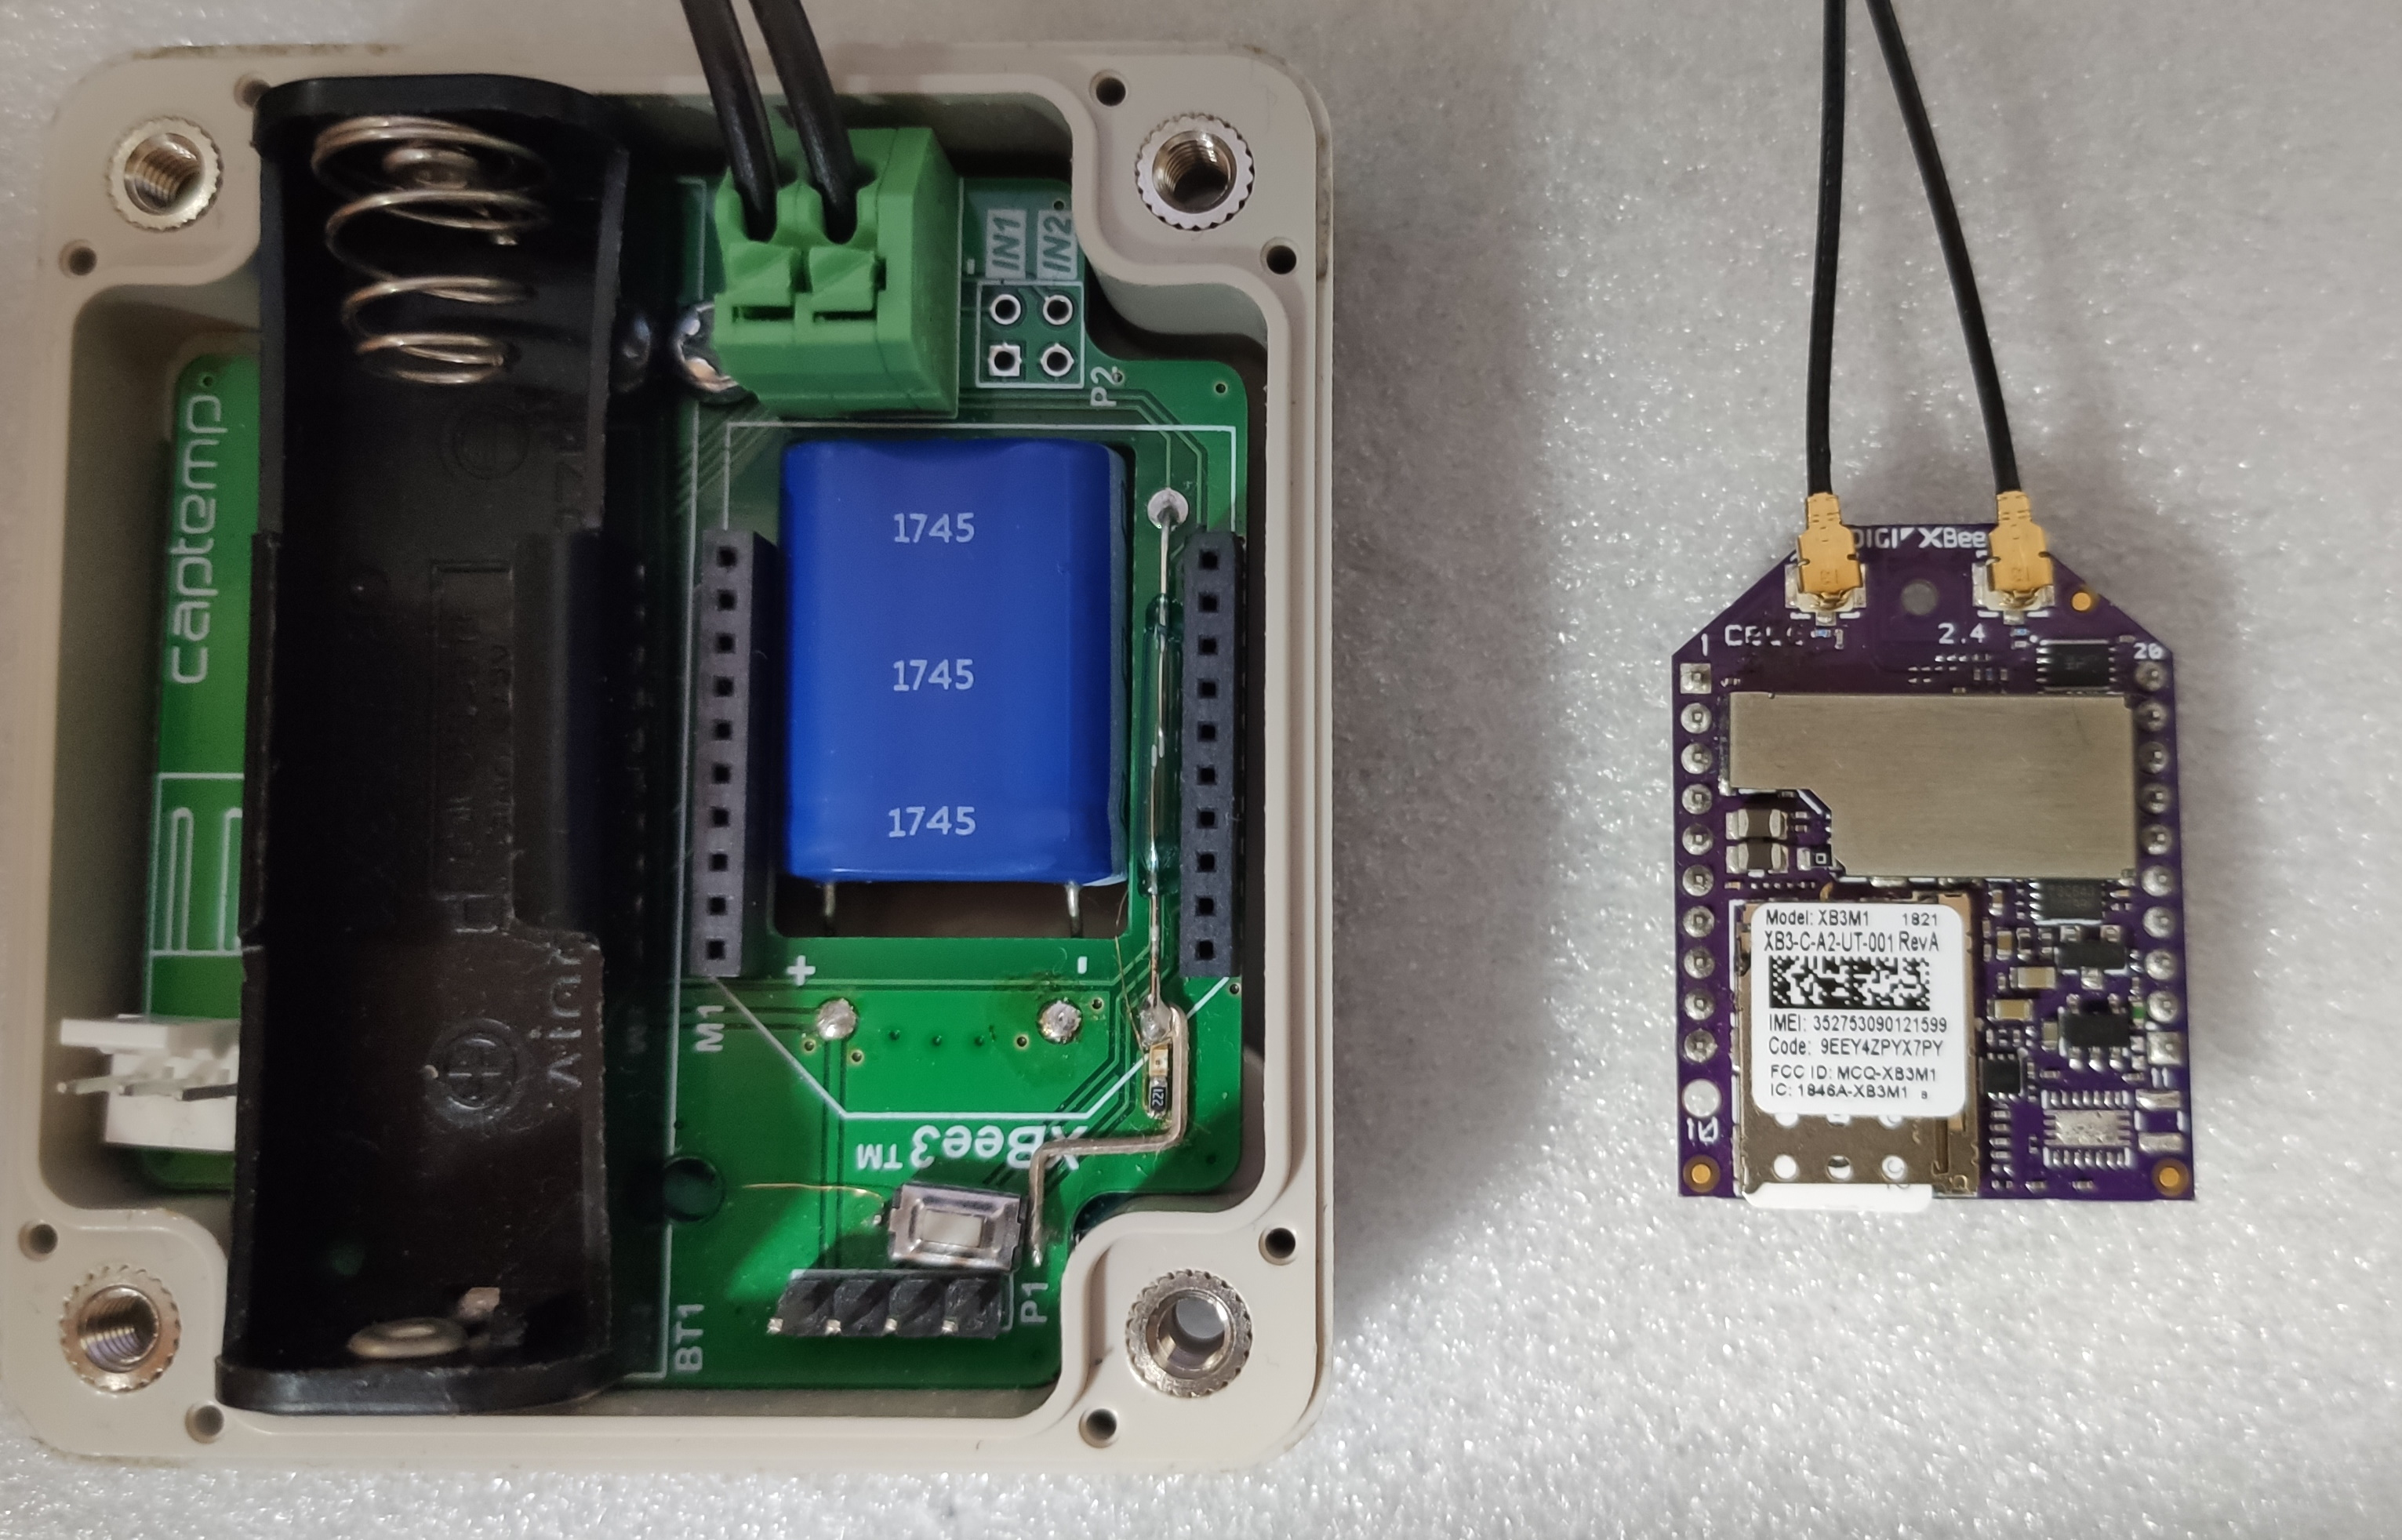
\includegraphics[width=0.60\textwidth]{images/xbee.jpg}
\caption{Módulo Xbee 3 e placa de expansão desenvolvida pela Captemp}\label{figxbee}
\end{figure}

\begin{table}[htb]
\caption{Especificações do Módulo Xbee 3}\label{tab1}
\begin{tabular}{|c|c|}\hline
Chipset& U-blox SARA-R410M-02B\\\hline
Dimensões& 24.38 mm x 32.94 mm \\\hline 
Temperatura de Funcionamento& -40º C to +85º C \\\hline 
Tipo de SIM & 4FF Nano \\\hline
Interfaces& UART, SPI, USB \\\hline 
Programação MicroPython& 32 KB Flash / 32 KB RAM \\\hline 
I/O& 4 ADC (10-bit), 13 I/O digitais, USB, I2C \\\hline 
Bluetooth& BLE Ready \\\hline 
Potencia de Transmissão& Até 23 dBm \\\hline 
Sensibilidade de Receção (LTE-M) & -105 dBm \\\hline 
Sensibilidade de Receção (NB-IoT) & -113 dBm \\\hline 
Velocidade Downlink/Uplink(LTE-M) & Até 375 kb/s \\\hline 
Velocidade Downlink/Uplink(NB-IoT) & Até 27.2 kb/s Downlink, 62.5kb/s Uplink \\\hline 
Alimentação & 3.3-4.3VDC \\\hline 
Pico corrente na transmissão & \begin{tabular}{@{}c@{}} 550mA - Bluetooth OFF \\ 610mA - Bluetooth ON\end{tabular}\\\hline 
Corrente média de transmissão (LTE-M) & 235mA \\\hline 
Corrente média de transmissão (NB-IoT) & 190mA \\\hline 
Modo Power Save& 20uA \\\hline 
Modo Deep Sleep& 10uA \\\hline 
\end{tabular} 
\end{table}

\par A Captemp pretende, através da utilização deste módulo e de uma placa de expansão desenvolvida pela própria, apresentada anteriormente na figura \ref{figxbee}, desenvolver uma versão do seu outro equipamento de Nb-Iot, mais simples representando numa opção de menor custo para o cliente. Será necessário desenvolver todo o código referente à gestão interna de Logs para guardar informação quando não existe cobertura para envio, o agendamento do envio e leituras, otimização da memória e bateria e implementação de comunicação bidirecional com encriptação com o portal Senslive. Sempre com recurso á programação em MicroPython.
A placa de expansão inclui um módulo de RTC, um conversor 1Wire para possibilitar a leitura de sondas já desenvolvidas pela Captemp, um sistema de alimentação para possibilitar a alimentação por pilha ou por alimentação externa. Ao desenvolver todo o equipamento a empresa tem o controlo total sobre o Firmware e sobre a estrutura de envio e a vantagem de tornar o equipamento compatível com todos os sensores que já possui.

\subsection {MicroPython}
\par O MicroPython\cite{MicroPython}, lançado em 2014, é um compilador e interpretador que implementa a linguagem Python3 e otimiza o seu funcionamento em microcontroladores. Escrito em C e disponibilizado em Open-Source é possível adaptar o mesmo para os diversos equipamentos. \par
É suportado por diversas arquiteturas de processadores tais como:
\par
\begin{itemize}
\item x86
\item x86-64
\item ARM
\item ARM Thumb
\item Xtensa
\end{itemize}
\par
Em microcontroladores que suportem Multi-thread , não sendo o caso do módulo usado está disponível ao programador o módulo de "\_thread" para criar processamento paralelo. Disponibiliza a programação de interrupções físicas, uteis em microcontroladores, tem disponível um "Garbage collector" para gerir a memória do microcontrolador e bibliotecas tais como "usocket" para criação e gestão de sockets, "network" para gerir a comunicação com o módulo específico de cada microcontrolador, ou a biblioteca para gerir o módulo de Bluethooth denominada por "ubluetooth". As bibliotecas disponíveis encontram-se no Site oficial da documentação\cite{micropython_lib}. 

\subsection {NB-Iot/ LTE-M}
O NB-Iot ou Narrowband Iot  e o LTE-M são tecnologias de Low Power Wide Area. São indicadas para sistemas Smart em diversas áreas como a monotorização, a agricultura, localizadores entre outras áreas. Similar ao funcionamento da rede móvel, onde cada equipamento possui um cartão SIM e se liga á rede fornecida pelo operador, mas utilizado em equipamentos com menor transmissão de dados e que não tem acesso a fontes de alimentação fixas e requerem de baterias, o NB-Iot promete autonomias das baterias a rondar os 10 anos\cite{u_2017}.Devido ao baixo volume de dados o plano de dados é possível apenas com pequeno investimento obter anos e até décadas de transmissões de dados.
\par De entre as vantagens podem-se destacar:
\begin{itemize}
\item Baixo Consumo
\item Longo alcance e boa penetração
\item Baixo custo de desenvolvimento na implementação da cobertura
\item Custo reduzido pelas transmissões
\item Sem necessidade de Roaming
\end{itemize}
\par
A cobertura da rede está a ser implementada pelas operadoras de telecomunicações que já possuem cobertura da rede GSM e infraestrutura de ligação á rede Internet desenvolvida e apenas necessitam de 
disponibilizar cobertura nas antenas de rede móvel, normalmente já existe compatibilidade de Hardware e basta atualizações de Firmware. É aconselhado pelas operadoras que se utilize o Nb-Iot para equipamentos fixos e o LTE-M para equipamentos em movimento.

\subsubsection { Low Power Wide Area}
As redes Low Power Wide Area são redes usadas frequentemente no IOT quando é necessário enviar dados a distâncias longas. Combinam a largura de banda e o consumo de bateria presente em redes como BLE e Zigbee, com alcance igual ou superior às redes de comunicação GSM. São caracterizadas por ter longo alcance, um baixo custo de transmissão e baixo consumo, onde simples baterias podem fornecer alimentação na ordem das décadas. Este alcance pode ser conseguido por exemplo por redes multihop ou modulações especificas que privilegiem o consumo energético e o alcance. A comunicação 2G e 3G pode ser usada em comunicação M2M mas as mesmas tem uma largura de banda superior ao necessário o que resulta em consumo de bateria excessivo onde não é tirado proveito da largura de banda disponível. Alguns exemplos de redes Low Power Wide Area, ou simplesmente denominadas por LPWAN, são o DASH7, o SigFox, LoRa, Ingenu, Telensa ou o NarrowBand Iot.\cite{lpwanoverview}

\begin{figure}[ht]
\centering
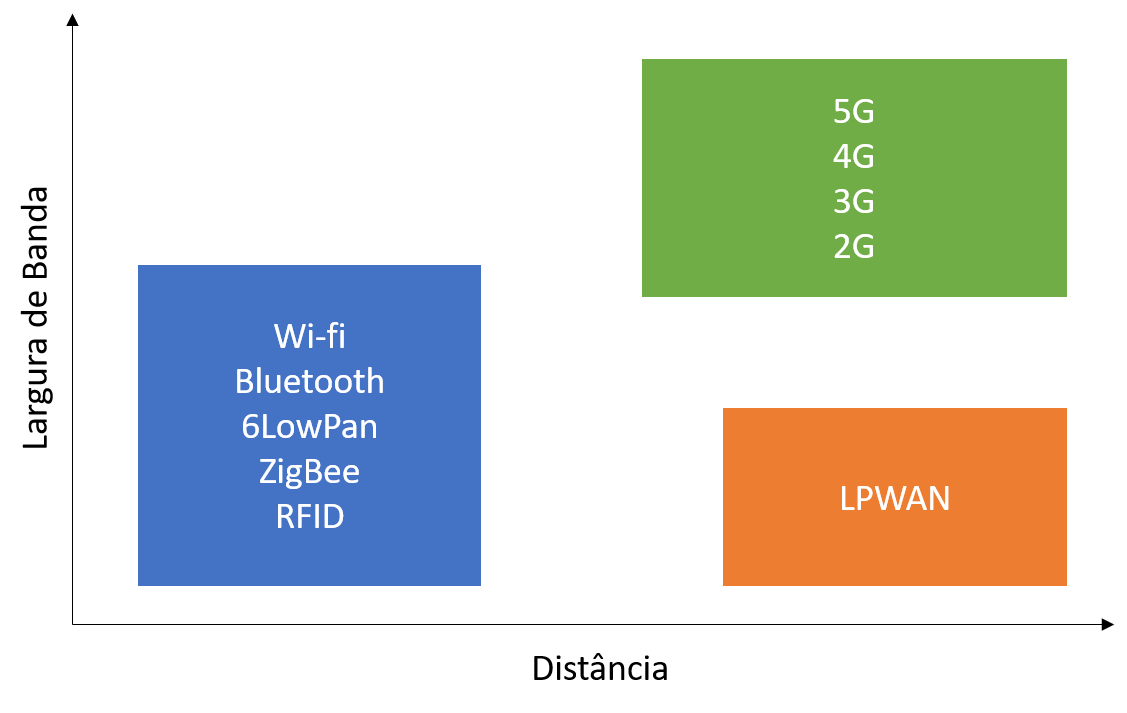
\includegraphics[width=0.45\textwidth]{images/lpwan.png}
\caption{Gráfico com relação Distancia vs Largura de Banda\cite{masterthesisLPWAN}}\label{figgraphlpwan}
\end{figure}



\section {Kea Tracker}\label{kea}
O Projeto Kea Tracker utiliza Beacon’s da Ruuvi, uma Beacon open-source\cite{ruuvi}, que disponibiliza de forma open-source tanto o Firmware para alterações, como as aplicações para Android e IOS. Será desenvolvida uma aplicação baseada na aplicação fornecida e o Firmware para disponibilizar a funcionalidade de data-logger.
\subsection{Beacons BLE}
\par
O Bluetooth Low Energy ou simplesmente BLE foi desenvolvido a pensar nos novos equipamentos IOT, onde os utilizadores querem vários equipamentos ligado ao mesmo tempo. Para tal foi desenvolvido o BLE que permite mais ligações ao mesmo tempo comparando com o Bluetooth clássico.
Como é indicado no nome, o principal fator diferenciador nesta versão, utilizada muitas vezes em equipamentos IOT, é o baixo consumo de aproximadamente metade relativamente ao Bluetooth normal. Outras características melhoradas a visar os equipamentos de IOT no BLE são a baixa largura de banda e o baixo tempo de transmissão.

Com o desenvolver do BLE foram criados, novos tipos de equipamentos, nomeadamente as beacons, equipamentos quase sempre alimentados por pilhas, que comunicam através de BLE, tornando o equipamento portátil. As beacons são caracterizadas por transmitir pequenas quantidades de informação em Broadcasting.
Existem dois tipos de beacons as beacons não conectáveis e as conectáveis\cite{blepacket}. Como indicado no nome as beacons conectáveis permitem que um equipamento (como um smartphone) se conecte á beacons e esta fica preparada para receber dados. As não conectáveis apenas permitem o broadcasting dos dados, poupando energia pois apenas é necessário ter o módulo acordado para fazer o broadcast e o restante do tempo podem estar num estado sleep. Na figura \ref{blepacket} é apresentado o pacote que é transmitido em broadcast para os outros equipamentos ao alcance.

\begin{figure}[htb]
\centering
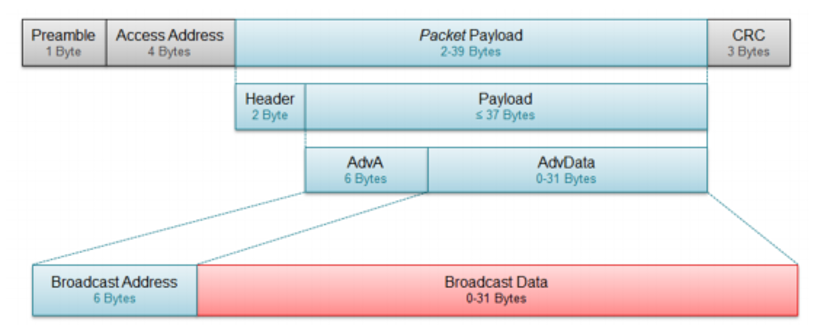
\includegraphics[width=0.65\textwidth]{images/blepacket.png}
\caption{BLE Broadcast packet\cite{blepacket}}\label{blepacket}
\end{figure}


\subsection{Ruuvi Beacons}
\par Neste projeto o firmware das beacons necessita de uma alteração, tornar a beacon numa beacon conectável e esta armazenar internamente as últimas leituras num buffer circular e criar um data-logger e caso o cliente pretenda poderá conectar mais tarde para fazer o download para aplicação e posterior envio para o Senslive, não necessitando a proximidade do smartphone á beacon durante todo o tempo. A Ruuvi dispõe de dois modos de desenvolvimento de firmware da beacon em C ou usando o Espruino, á semelhança do MicroPython um interpretador de JavaScript para microcontroladores lançado em 2012, totalmente compatível com as beacons da Ruuvi.
\subsection{Apps Smartphones}
Na fase inicial será adaptada a versão disponibilizada para Android para agilizar a integração com o portal Senslive. A aplicação base para android disponibilizada pela Ruuvi foi desenvolvida em Kotlin\cite{ruuviappgithub}, uma linguagem desenvolvida pela JetBrains multiplataforma e que inclui o Android nessas plataformas compatíveis.
De seguida estão apresentadas algumas alterações necessárias na aplicação:
\begin{itemize}
\item Alteração das Imagens e Logotipo da App;
\item Alteração do Nome da App;
\item Remoção de conteúdo não necessário;
\item Bloqueio do URL de envio para usar exclusivamente o portal Senslive;
\item Melhoramento da precisão da posição GPS;
\item Possibilidade da alteração dos intervalos de registo
\end{itemize}

\section {dot.Tracker}\label{dot}
Á semelhança do projeto Kea Tracker o projeto dot.Tracker usa igualmente beacon's BLE para enviar a informação necessária para o respetivo portal. É necessário recolher os pacotes recebidos das beacons enviá-los para o servidor e calcular a distância entre a beacon e o receptor e com o auxilio de múltiplos recetores realizar a triangulação da beacon num mapa. No decorrer do projeto será necessário desenvolver uma plataforma web para receber e visualizar as localizações provenientes das beacons e respetivas configurações, adotar o método de algoritmo para a triangulação da beacon relativamente a vários recetores e realizar testes ao funcionamento e precisão do sistema.
\subsection{Beacons e gateway}
 Para este projeto irá ser utilizado durante o desenvolvimento a solução da Beacon Line\cite{taskit} e posteriormente desenvolvido recetores propriétarios da Captemp. A solução apresentada pela Beacon Line, é composta por um gateway e vários nós. Cada nó possui um recetor BLE e quando o mesmo recebe um broadcast proveniente da beacon o transmite para o gateway. Caso exista alguma divergência da potência de transmissao desde o último pacote enviado por essa mesma beacon o gateway com connectividade Ethernet realiza o publish num broker onde é possível o servidor obter os pacotes das beacon's.



\section{Soluções e Tecnologias Disponíveis} \label{solucoesDisponiveis}
\subsection{Tecnologias Disponíveis}
\subsubsection{Compressão de Ficheiros}
\par
Atualmente a vida online do Homem passou a ter um grande impacto na sua vida. Para tal as páginas web e seus conteúdos foram aumentado em quantidade e tamanho e com menores tempos de resposta. Isso é aplicável tanto aos ficheiros que contem o layout da página, quer das imagens. Para poupar dados de transmissão e reduzir tempos de envios, ou simplesmente suportar larguras de banda inferiores, os browsers integraram a possibilidade de receber os ficheiros comprimidos e fazer a descompressão para mostrar ao cliente quase em tempo real. Atualmente os browser recentes suportam a compressão por GZIP( já utilizado na página do equipamento Nidus) e compressão utilizado a codificação Brotlin \cite{Alakuijala2019} \cite{brotlirfc}.
Cada método de compressão possui as suas vantagens e desvantagens, o brotli por sua vez á semelhança de outros métodos em comparação com o GZIP, tem uma taxa de compressão superior\cite{Alakuijala2015}, isto significa que consegue reduzir o mesmo ficheiro no seu respetivo ficheiro comprimido ocupando menos espaço em relação ao GZIP, mas como desvantagem o tempo de compressão do mesmo é superior. Ao contrário da compressão, na descompressão o Brotli tem melhores resultados do que nas restantes alternativas apresentando velocidades superiores de descompressão.
\par
O GZIP e o brotli usam na sua compressão para reduzir o tamanho do ficheiro o algoritmo de compressão LZ77, que procura sequências repetidas utilizando o método de janela deslizante e substitui essas sequências por referências para a primeira ocorrência que não foi substituída indicando a distância a que a primeira ocurência ocorre e o tamanho a substitui.
\par O sistema de janela deslizante define um tamanho da janela e ao deslocar a janela do tamanho definido define um dicionário. Após definir o dicionário com vários tamanhos de janelas, percorrer novamente o ficheiro através do método de janela deslizante novamente a procurar repetições das entradas que existem no dicionário. Quando uma sequência é encontrada esta é substituída  por uma referência da posição da primeira ocurrência da mesma. Na figura \ref{janela} é apresentado um exemplo do funcionamento da janela deslizante para a obtenção do dicionário com o tamanho da janela a variar de 2 a 7.
\begin{figure}[htb]
\centering
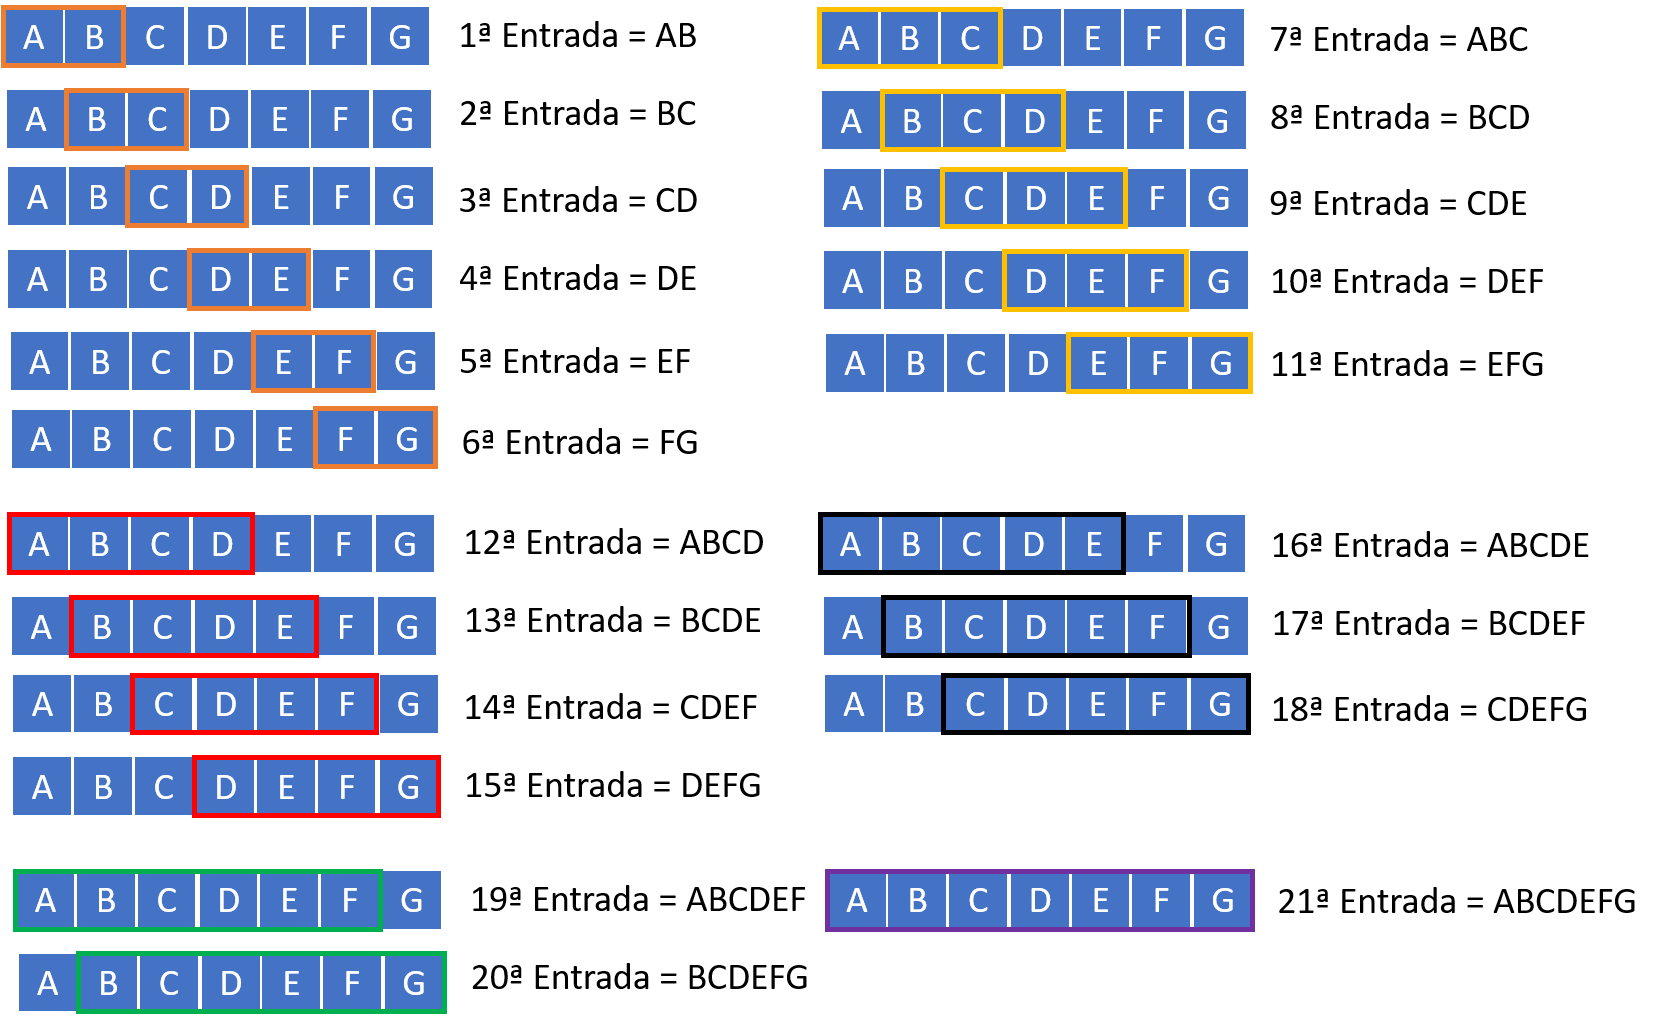
\includegraphics[width=0.85\textwidth]{images/janeladeslizantedicionario.png}
\caption{Funcionamento da Janela Deslizante}\label{janela}
\end{figure}


\par Na figura \ref{gzip} e \ref{gzip2} é apresentado dois exemplos visuais e simples utilizando frases de como o LZ277, usado pelo GZIP e Brotl através do sistema de janela deslizante procura as repetições e comprime os ficheiros. Na Figura \ref{unzip} é apresentado o ficheiro base, representado por um pequeno texto. No exemplo apresentado pela figura \ref{gzip} apenas foi utilizado a substituição de palavras inteiras, na figura \ref{gzip2} procura sequências de caracteres sejam elas palavras ou não. Nos exemplos apresentados a redução foi de 20\% [$1-\dfrac{48}{60}\times100\%$] no primeiro exemplo e de aproximadamente de 32\% [$1-\dfrac{41}{60}\times100\%$] no segundo.
\begin{figure}[htb]
\centering
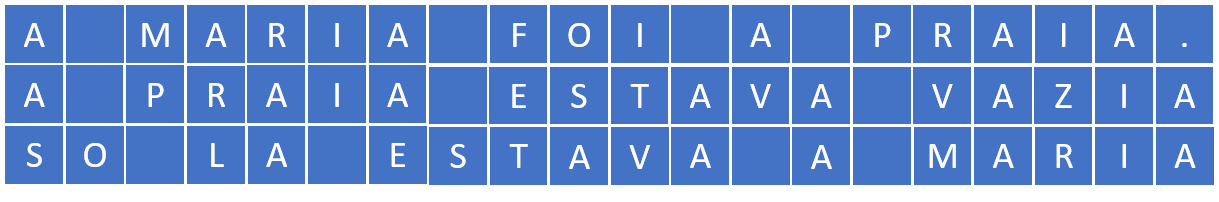
\includegraphics[width=0.85\textwidth]{images/FILE.png}
\caption{Sequência não comprimida}\label{unzip}
\end{figure}

\begin{figure}[htb]
\centering
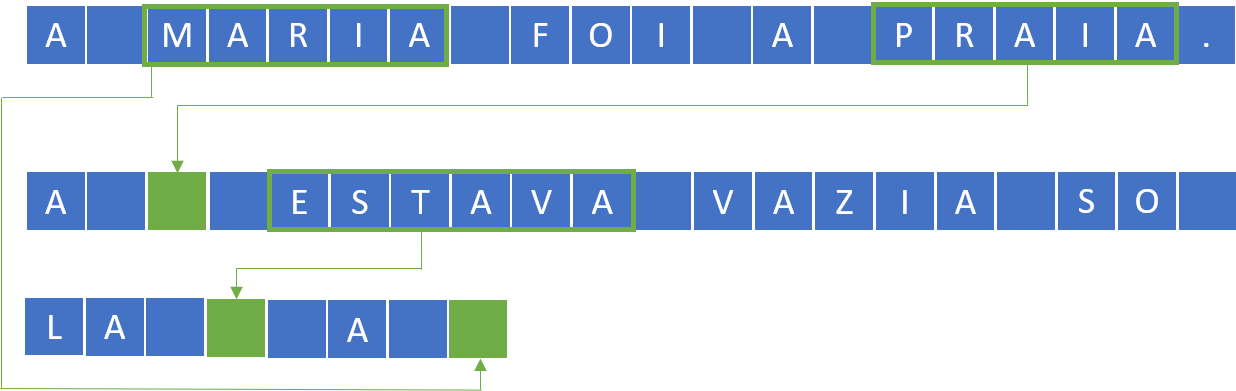
\includegraphics[width=0.85\textwidth]{images/gzip.png}
\caption{Sequência comprimida com LZ77 (apenas palavras)}\label{gzip}
\end{figure}
\begin{figure}[htb]
\centering
\includegraphics[width=0.85\textwidth]{images/gzip2.png}
\caption{Sequência comprimida com LZ77(palavras e sequências)}\label{gzip2}
\end{figure}


\subsubsection{Compressão de Imagens}
\par

O utilizador pretende igualmente ver as imagens com a máxima qualidade, mais qualidade significa um maior detalhe e por sequencia um ficheiro de maior tamanho. Existem atualmente vários softwares online e locais que reduzem o tamanho das imagens. Na conceção da página da Nidus é utilizado o website TinyPNG.com que analisa a imagem original e converte as cores em cores mais simples de o sistema armazenar, como por exemplo uma imagem com 24 bits de profundidade de cor pode ser convertido em uma similar com apenas 8 bits reduzindo o tamanho do ficheiro e impercetível para o olho humano num ecrã\cite{Hilles2019}. Alternativamente ao Tiny Png existem softwares, similares alguns de licença GNU/GPL, para comprimir imagens. Com o "Mass Image Compressor"\cite{Mass_Image_Compressor}(apenas um exemplo), é possível comprimir as imagens com a possibilidade de indicar a quantidade de compressão.
\par
Com a enorme quantidade e diversidade de monitores existentes, as páginas web necessitam de ser responsivas e apresentar a melhor imagem para o monitor em questão, isso normalmente traduz-se em várias versões similares da imagem alojadas no servidor. No caso dos microcontroladores e sistemas embebidos o espaço encontra-se limitado e deve-se arranjar uma solução. Uma solução possível é ao invés da utilização de imagens PNG, JPG ou outras, é a utilização de imagens em SVG, onde a imagem é representada por um ficheiro XML que descreve uma imagem bidimensional e utiliza na sua constituição modelos matemáticos para o cálculo das posições dos elementos. Com isto é possível manipular o XML em tempo real para alterar elementos ou remover, alterar cores, criar animações entre outras. Inclui a vantagem de como a imagem é representada por formulas matemáticas, é possível escalar a imagem sem perder qualidade, pois a função matemática é ajustável. Num sistema embebido como o caso da Nidus é vantajoso a utilização de imagens em SVG para criação das animações. Atualmente as animações da página da Nidus são criadas com várias imagens PNG comprimidas e convertidas em base64 e são alternadas no HTML pelo JavaScript. Com a utilização de imagens SVG é possível ter apenas uma imagem alojada e manipular a imagem em tempo real através do JavaScript de uma forma mais suave para o utilizador, pois apenas a zona a alterar é alterada na imagem.
Á semelhança dos JPG e PNG o SVG também pode ser comprimido, para tal basta no XML da imagem remover os meta-dados  e utilização de funções matemáticas mais simples, não necessários para o browser apresentar a representação gráfica do mesmo, mas os softwares de edição adicionam para funcionalidades exclusivas do editor. Á semelhança dos ficheiros HTML após a remoção dos meta-dados o ficheiro pode ser minificado.

\subsubsection{Localização indoor}
\par
É possivel encontrar na comunidade científica vários estudos sobre a utilização de redes Wi-Fi e Bluetooth para sistemas de localização. Estes mesmos focam-se no cálculo das distâncias do equipamento para vários recetores no mesmo intervalo temporal, algumas destas soluções baseiam-se nos valores de RSSI da transmissão e o valor definido como constante da potência de transmissão á distância de 1 metro, e estimar a sua distância aproximada de cada recetor, com essas aproximações é possivel através do algoritmo escolhido\cite{Wang2013}, obter a estimativa da localização do equipamento e a sua colocação num mapa.
A distância de um recetor para o emissor baseada no  valor de RSSI é expressa pela seguinte formula, onde dbm é a constante da potência de transmissão da beacon a 1 metro, n a constante do ambiente e o RSSI corresponde ao RSSI da transmissão:
\par
\begin{center}
  $d=10^(\frac{dbm-RSSI}{10 \times n})$
\end{center}

\par
Após a obtenção da distância para cada recetor é possível  aplicar um algoritmo para estimar a localização. Os mais referenciados e adotados são o centroid baseado no centro geométrico do polígono formado pelas interceções das circunferências criadas com o raio da distância calculada pela fórmula anteriormente apresentada, o método Three-border Positioning e o Least Square Estimation.
Como é possivel observar na figura \ref{centroid} utilizando o método do centroid, o centro geométrico corresponde á localização do equipamento com base nos recetores. A formula que representa o centro utilizando o centroid é expressa pela seguinte equação onde n representa o numero de recetores utilizados no cálculo.
\par
\begin{center}
$ (x,y)= (\frac{x_{1}+x_{2}+x_{3}+...+x_{n}}{n},\frac{y_{1}+y_{2}+y_{3}+...+y_{n}}{n})$
\end{center}

\begin{figure}[htb]
\centering
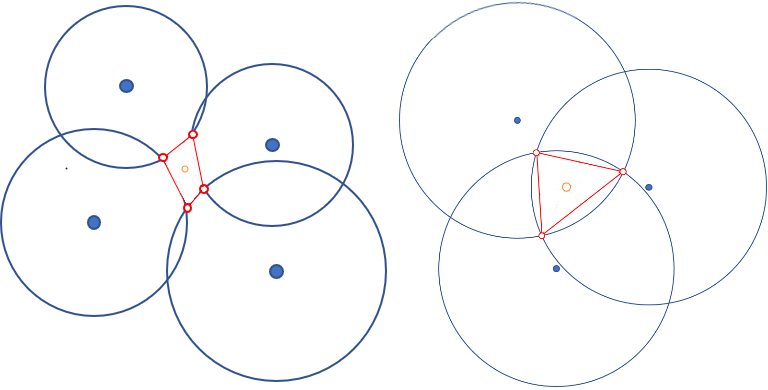
\includegraphics[width=0.95\textwidth]{images/centroid3.png}
\caption{Posição utilizando o método Centroid com 3 e 4 recetores}\label{centroid}
\end{figure}

Ao invés da utilização do método do centroid se for adotado o método Three-border Positioing, é criada a função definida por ramos composta pelas três equações da circunferência A, B e C com os respetivos centros em cada recetor e com o raio igual á distância calculada para esse mesmo recetor. Para calcular a posição estimada é calculado o resultado dessa mesma função de modo a encontrar o ponto x,y que representa a posição do equipamento.
\par 
Utilizando o método Least Sqare Estimation ou simplesmente LSE e á semelhança do Three-border Position\cite{Zhu2014} é criada a função de ramos das equações das circunferências dos vários recetores com o raio da distância calculada, mas pode igualmente como o centroid utilizar mais do que três recetores aumentando a precisão. \par Hua, Z., Hang, L., Yue, L., Hang, L., \& Kan, Z. (2014). Geometrical constrained least squares estimation in wireless location systems. 2014 4th IEEE International Conference on Network Infrastructure and Digital Content. apresenta os passos necessários calcular a posição X do equipamento através do método LSE. Em primeiro são criadas a função de ramos composta pelas equações das circunferências com centro nos recetores ([$x_{1}$,$y_{1}$],[$x_{2}$,$y_{2}$],[$x_{3}$,$y_{3}$],[$x_{4}$,$y_{4}$]) e o raio igual á distância calculada($d_{1}$,$d_{2}$,$d_{3}$,$d_{4}$).
\begin{center}
\[
  \begin{cases}
      (x_{1} -x)^2 + (y_{1}-y)^2 = {d_{1}}^2\\
      (x_{2} -x)^2 + (y_{2}-y)^2 = {d_{2}}^2\\
      (x_{3} -x)^2 + (y_{3}-y)^2 = {d_{3}}^2\\
      (x_{4} -x)^2 + (y_{4}-y)^2 = {d_{4}}^2\\
  \end{cases}
\]
\end{center}

\par Após a criação da função é subtraido o primeiro ramo aos restantes ramos e a função reduz o numero de ramos para n-1 onde n representa o numero de recetores a usar na função.
\begin{center}

\[
  \begin{cases}
     2(x_{2}-x_{1})x+2(y_{2}-y_{1})y={x_{2}}^2-{x_{1}}^2+{y_{2}}^2-{y_{1}}^2+{d_{2}}^2+{ d_{1}}^2\\
     2(x_{3}-x_{1})x+2(y_{3}-y_{1})y={x_{3}}^2-{x_{1}}^2+{y_{3}}^2-{y_{1}}^2+{d_{3}}^2+{ d_{1}}^2\\
     2(x_{4}-x_{1})x+2(y_{4}-y_{1})y={x_{4}}^2-{x_{1}}^2+{y_{4}}^2-{y_{1}}^2+{d_{4}}^2+{ d_{1}}^2\\
  \end{cases}
\]
\end{center}
\par A função pode ser representada pelo seu equivalente numa representação de matrizes por $2AX = b$ onde.

\begin{center}



$A=\begin{bmatrix}
x_{2}-x_{1} & y_{2}-y_{1}\\
x_{3}-x_{1} & y_{3}-y_{1}\\
x_{4}-x_{1} & y_{4}-y_{1}
\end{bmatrix}$

$B=\begin{bmatrix}
b_{1}\\
b_{2}\\
b_{3}
\end{bmatrix}=\begin{bmatrix}
{x_{2}}^2-{x_{1}}^2  + {y_{2}}^2-{y_{1}}^2 - {d_{2}}^2 + {d_{1}}^2 \\
{x_{3}}^2-{x_{1}}^2  + {y_{3}}^2-{y_{1}}^2 - {d_{3}}^2 + {d_{1}}^2 \\
{x_{4}}^2-{x_{1}}^2  + {y_{4}}^2-{y_{1}}^2 - {d_{4}}^2 + {d_{1}}^2 \\
\end{bmatrix} $

\end{center}

\par A posição estimada do equipamento representada no exemplo por X é definida por:



\par
\begin{center}
$ X= \frac{1}{2}(A^T A)^{-1} A^T b$
\end{center}

\par Os testes analisados demonstram\cite{Wang2013} , que o método LSE é o método que obtem os melhores resultados com os valores mais próximos do real. No teste apresentado em segundo lugar está o Three-border Position e por último o Centroid. Com algumas discrepâncias em algumas das amostragens.

\subsection{Produtos Similares}
\subsubsection{NB-Iot}
\par
Atualmente no mercado começam a surgir alguns produtos similares ao que se pretende desenvolver como é o caso dos sensores da Efento\cite{epoka}, que disponibiliza vários tipos de sensores que comunicam por NB-Iot. A Efento é uma empresa fundada em 2014 e é focada em desenvolvimento de equipamentos IOT. Atualmente desenvolveram versões com suporte para NB-Iot. Estes equipamentos tem a desvantagem de não ser compatível com o pacote de envio desenvolvido no portal Senslive e apenas permite o envio para o portal da Efento e não existe a possibilidade da utilização das sondas já comercializadas pela Captemp. Como vantagem á semelhança do equipamento a desenvolver é a utilização de um sistema com Log para quando não existe possibilidade de comunicação.
Devido ao desenvolvimento da tecnologia ainda existem poucas soluções em comercialização, estando as mesmas em desenvolvimento. A Captemp possui igualmente outro equipamento, completamente desenvolvido pela empresa, em desenvolvimento que tira partido do NB-Iot com o acréscimo em relação ao que se pretende desenvolver durante o estágio, a possibilidade de ter mais sensores, maior capacidade de Log interno, configuração por Bluetooth, GPS e um Display integrado como extra.
\subsubsection{Kea Tracker}
Após pesquisas online é possível encontrar algumas soluções de beacons que permitem o armazenamento interno de leituras para desenvolver um sistema de data-logger tais como a Beacon da Fujitsu, a FWM8BLZ02A-109069\cite{beacon1} , á semelhança da beacon da Ruuvi usa o mesmo chip o nRF52832 da Nordic Semiconductor, mas apresenta como vantagens a inclusão de um sistema de Logs interno com capacidade para aproximadamente 4080 leituras e a diversidade de sensores já incluídos. Como desvantagem em relação á Beacon da Ruuvi tem a inclusão de um sensor de temperatura ao invés de temperatura e humidade, não possui sensor de pressão atmosférica e não é open-source possuindo um firmware fechado. A vantagem de se desenvolver um produto desde a sua raiz é a possibilidade de ter o controlo total sobre a solução para posteriores melhoramentos e ter a solução a desempenhar apenas o que pretendemos.
\par
Outra solução existente no mercado é igualmente a solução da Blue Maestro que possui variadas versões de beacons. Á semelhança da Beacon da Fujitsu possuem igualmente sistema de Log. Contrariamente á FWM8BLZ02A-109069 é uma beacon que tem disponível em Open-Source uma API e um SDK para desenvolver as nossas aplicações. Comparada com a beacon da Ruuvi, a Ruuvi beacon é completamente open-source e não apenas a API para comunicação.
\par
Na tabela \ref{tabbeacons} são apresentadas as diferenças e semelhanças entre os três modelos analisados

\begin{table}[htb]
\caption{Comparação entre beacons \cite{specsrect}\cite{bluespecs}\cite{ruuvispecs}}\label{tabbeacons}
\begin{tabular}{|c|c|c|c|}\hline
& Ruuvi Tag& Fujitsu Beacon &Blue Maestro \\\hline
Processador& nRF52832& nRF52832 &? \\\hline
Memória&\begin{tabular}{@{}c@{}}512kB Flash \\ 64kB RAM\end{tabular} & 32K Não volátil &?\\\hline 
Protocolos&\begin{tabular}{@{}c@{}c@{}@{}c@{}} Bluetooth 5 \\ Wirepass \\ Mira OS\\QUUPA\\Others (2.4GHz)\end{tabular}&Bluetooth 4.1&BLE 4.2\\\hline 
\begin{tabular}{@{}c@{}}Potência de\\ Transmissão\end{tabular} &+4 dBm &\begin{tabular}{@{}c@{}}-16, -12, -8\\ -4, 0, +4 dBm\end{tabular} &-4, 0, +4 dBm \\\hline
Sensores& \begin{tabular}{@{}c@{}c@{}c@{}} Acelerometro\\ Temperatura\\ Humidade \\Pressão\end{tabular} &\begin{tabular}{c@{}c@{}} Acelerómetro\\ Temperatura\end{tabular}&\begin{tabular}{@{}c@{}c@{}} Temperatura\\ Humidade \\Pressão\end{tabular}\\\hline 
NFC & \checkmark&- &-\\\hline
Bateria &\begin{tabular}{@{}c@{}}CR2477\\ 1000mAH - Li/MnO2\end{tabular}&CR2450 &CR2032\\\hline
\begin{tabular}{@{}c@{}}Autonomia\\(espetável)\end{tabular}& ~10 Anos&1 Ano em Broadcast &\begin{tabular}{@{}c@{}}1 Ano em Broadcast\\2 Anos com Log\end{tabular}\\\hline
Data Logger &\begin{tabular}{@{}c@{}}-\\(a desenvolver)\end{tabular}&\checkmark &\checkmark\\\hline
Open Source & \checkmark&- &\checkmark ( API \& SDK )\\\hline
Informações & \begin{tabular}{@{}c@{}c@{}@{}} IP67 \\ 2 Botões\\2 Leds\\52mm \diameter\\\end{tabular}&\begin{tabular}{c@{}c@{}} Led\\ 40 x 31 x 12mm \end{tabular}&\begin{tabular}{@{}c@{}}24000 Registos\\33mm \diameter\end{tabular} \\\hline
\end{tabular} 
\end{table}
\par


\clearpage \cleardoublepage %!!!!!!!!!!!!!!!!!!!!!!!!!!!!!!!!!!!!!!!!!!!!!!!!!!!!!!!!!!!!!!!!!!!!!!!!!!!!!!!!!!!!!!!!!!!!!!!!!!

\chapter{Trabalho Desenvolvido}\label{workcharp}
\section{Introdução}
Nesta secção é apresentado o trabalho e desenvolvimento dos projetos realizados durante o estágio e á semelhança do capítulo anterior cada projeto será desenvolvido num subcapítulo dedicado.

\section{Coletor de dados - Nidus} 
\par Durante o estágio o projeto referente ao coletor de dados Nidus apresenta 5 subsecções a tratar, o desenvolvimento do sistema de tradução para a página do equipamento no menor espaço de memória possível, o desenvolvimento de páginas com layouts específicos, a correção de \textit{Bug's} que possam existir e venham a ser descobertos, a compressão dos ficheiros e imagens e melhorar/manter a página com layouts e funcionalidades de acordo com a concorrência e atualidade. Cada um dessas subsecções serão abordadas em cada subsecção seguinte.

\subsection{Sistema de tradução automática}
\par Os sistemas de internacionalização das páginas web, fornecem ao utilizador final um sistema com tradução automática para a língua pretendida, são cada vez mais utilizados. Isto acarreta um acréscimo da complexidade do sistema e por consequência o acréscimo do escaço ocupado pelo código. O sistema utilizado no caso particular das páginas web com JavaScript é o I18N, uma \textit{Framework} desenvolvida em JavaScript, com várias funcionalidades além da tradução de páginas. Estas funcionalidades extras não necessárias para o projeto apenas acarretam o aumento do peso do plugin no sistema, diminuindo possibilidades futuras de alterações e novos desenvolvimentos. Para tal será desenvolvido de raiz um sistema similar ao I18N apenas com as funcionalidades pretendias de modo a ser possível comparar a diferença de espaço ocupado.


\subsubsection{O funcionamento}
\par Os sistemas de tradução são baseados numa função chamada no momento necessário da obtenção de uma tradução onde é passado um parâmetro indicando qual a tradução pretendida. Esta função é responsável por percorrer o conjunto de traduções da língua selecionada e através de um sistema associativo chave-valor retornar caso este exista o valor para a chave fornecida. Caso este não exista é devolvido o valor \textit{default}, por normal a chave do mesmo. Na figura \ref{i18n} é apresentado o esquema do funcionamento do sistema de tradução descrito acima.

\begin{figure}[ht]
\centering
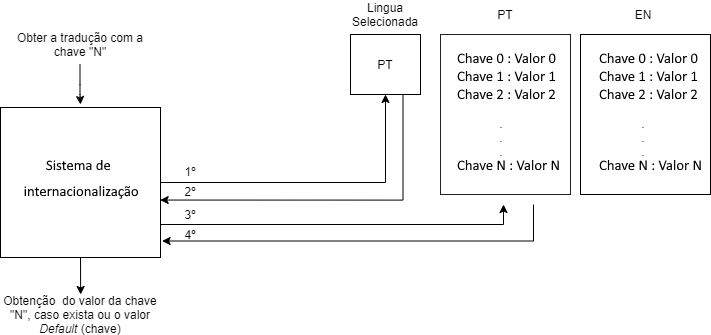
\includegraphics[width=0.95\textwidth]{images/i18n.png}
\caption{Processo da obtenção da tradução de um valor}\label{i18n}
\end{figure}

\par Após análise as funcionalidades requeridas para o projeto Nidus, são as seguintes:

\begin{itemize}
\item Tradução automática da página
\item Armazenamento persistente da linguagem escolhida
\item Alteração da linguagem pretendida, mediante a lista de opções
\item Carregamento das linguagens dinamicamente.
\end{itemize} 

\par De modo a armazenar a linguagem, esta estará alocada no browser sob a forma de uma \textit{cookie}. No momento de uma tradução, o sistema verifica o valor da \textit{cookie} em vigor e procura na associação chave-valor respetiva á linguagem selecionada, se a chave pretendida existe e caso exista o valor desta é devolvida. Caso a \textit{cookie} não exista é devolvida a opção \textit{default}.

\par O Sistema é composto por 4 funções. A primeira, gLng, responsável por verificar se existe a \textit{cookie} no \textit{browser} e retornar o seu valor ou o valor da língua \textit{default} o Inglês ("EN"). A segunda função, sLng, é utilizada aquando do guardar da linguagem para posterior utilização, esta como parâmetros recebe o valor a inserir, esta \textit{cookie} fica disponível no \textit{browser} durante 365 dias após a sua última atualização. Após guardar a \textit{cookie}, a página é recarregada de modo a atualizar todos os campos e não apenas os gerados a partir do momento da seleção da nova língua, garantindo que a página tenha várias línguas no mesmo instante de tempo. A terceira função "\_" é responsável por retornar o valor da chave fornecida no único parâmetro da mesma. Caso a chave não exista na língua selecionada pela \textit{cookie} é retornado o valor de \textit{default}, correspondente á chave fornecida como parâmetro da função. Por último existe a função "ll" com dois parâmetros, como primeiro parâmetro temos a \textit{string} correspondente ás iniciais da língua a adicionar (Exemplo: "PT","EN","ES","FR") e o segundo parâmetro um objeto com associações chave-valor para a língua fornecida. Esta função é responsável por adicionar ao conjunto de dicionários a língua pretendida ou atualizar o dicionário da língua caso este já exista.
\par O conjunto de dicionários armazenado segue o esquema apresentado na figura \ref{dicextr}. No caso de apenas se pretender desenvolver numa língua é possível apenas fazer a definição das funções e não fornecer nenhum dicionário, visto nesse caso ele devolver a chave, bastando para isso a chave corresponder á tradução pretendida na única língua disponível.



\begin{figure}[ht]
\centering
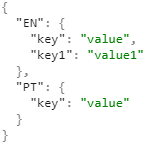
\includegraphics[width=0.25\textwidth]{images/extrjson.png}
\caption{Estrutura JSON do conjunto de dicionários}\label{dicextr}
\end{figure}

\par No excerto seguinte é apresentado o código referente ás funções criadas para o sistema.
\begin{verbatim}
1  var _d={}; //Dicionários
2  function gLng() {
3      var v = document.cookie.match('(^|;) ?locale=([^;]*)(;|$)');
4      return v ? v[2].toUpperCase(): "EN";
5  }
6
7  function sLng(v) {
8      var d = new Date;
9      d.setTime(d.getTime() + 31536000000);
10    document.cookie ="locale=" + v + ";path=/;expires=" +
   d.toGMTString();
11    location.reload();
12 }
13
14 function _(k){
15     if(_d==null|| _d==undefined || cd==undefined || cd==null ||
   _d[gLng()]==null || _d[gLng()]==undefined) {return k;}
16         return _d[gLng()][k];
17 }
18
19 function ll(a,b){
20     if(_d==null|| _d==undefined){ _d={};}
21         _d[a]=b;
22 }

\end{verbatim}

\subsubsection{Resultados obtidos}
\par Após comparação do sistema implementado em comparação com o I18N\cite{i18n} é possível observar a redução do tamanho para cerca de 34 \% ( 1178b - 66\% = 404b), este valor foi obtido na comparação entre as duas versões minificadas e comprimidas com o GZIP como é possível observar no gráfico apresentado na figura \ref{garph1}, no gráfico é possível verificar os tamanhos originais, após a minificação e o tamanho do minificado após a compressão com o GZIP. Ambos valores relativos à comparação não contemplam os dicionários, apenas o código inerente á utilização das funcionalidades.

\begin{figure}[ht]
\centering
\begin{tikzpicture}
\begin{axis}[
xbar,
height=5cm,width=10.8cm, 
y axis line style = { opacity = 0 },
axis x line = none,
tickwidth = 0pt,
enlarge y limits = 0.7, 
enlarge x limits = 0.02,
symbolic y coords = {I18N, Solução desenvolvida},
nodes near coords,
ytick=data,
legend style={
at={(rel axis cs:0.5,1)},
anchor=south,
legend columns=-1, 
column sep=2mm, 
draw=none 
}
]
\addplot coordinates { (6579,I18N) (575,Solução desenvolvida) };
\addplot coordinates { (2961,I18N) (427,Solução desenvolvida) };
\addplot coordinates { (1178,I18N) (404,Solução desenvolvida) };
\legend{Original, Minificado, Minificado+ GZIP}
\end{axis}
\end{tikzpicture}

\caption{Gráfico com comparação do tamanho entre versões (em Bytes)}\label{garph1}
\end{figure}

\subsection{Compressão de ficheiros}

\par Durante o estágio foi estudado igualmente a comparação entre a utilização do GZIP e do Brotli de modo a analisar as vantagens e desvantagens aplicadas ao projeto em questão.
\par Segundo estudos online \cite{brotlivsgzip}, é possível analisar que comparando apenas o Brotli e o GZIP, que este último tem uma taxa de compressão inferior, significa isto que o mesmo ficheiro após compressão é maior no caso do GZIP, tornando o Brotli um candidato a ponderar. Já no campo da velocidade de descompressão o caso inverte, sendo o GZIP a possuir melhores resultados, este parâmetro, não afeta o espaço ocupado na memória do microcontrolador. A velocidade de compressão é superior no Brotli não o tornando ideal para compressões em tempo real, mas visto o servidor WEB alojado na Nidus já possuir todos os ficheiros comprimidos e estes são sempre estáticos, o tempo de compressão não afeta o equipamento neste projeto. 
\par Visto o método Brotli possuir mais valias ao projeto, de modo a estudar e comparar as vantagens/desvantagens inerentes á migração para o Brotli, serão comprimidos os ficheiros atuais do projeto em ambos os métodos de modo a analisar os ganhos obtidos no projeto em especifico antes da sua atualização. Na tabela \ref{tabw2} são apresentados os resultados obtidos para cada ficheiro do projeto, os valores apresentados correspondem ao tamanho em bytes. No valor apresentado correspondente ao tamanho original, este no caso do HTML e CSS encontra-se minificado, caso seja JavaScript este encontra-se minificado e comprimido com recurso ao Google Clousure Compiler.


\begin{table}[htb]
\caption{Comparação entre Brotli e GZIP}\label{tabw2}
\begin{tabular}{|c|c|c|c|c|}\hline
Tipo do Ficheiro& \begin{tabular}{@{}c@{}} Tamanho original\\ Minificado\end{tabular} &Tamanho GZIP& Tamanho Brotli& Diferença \\\hline
JavaScript&230 304 & 58 061&52 453& -5 608 \\\hline
JavaScript&462 316& 95 196& 75 702& -19 494\\\hline
JavaScript&627 032& 221 754&206 150& -15 604 \\\hline
JavaScript&140 389 & 46 945& 42 687&-4 258\\\hline
JavaScript&84 249 & 28 579&26 594&-1 985\\\hline
HTML&37 302 & 16 728& 15 893&-835\\\hline
HTML&39 352 & 17 251& 16 348&-903\\\hline
FONT (.TTF)&111 368 & 66 831&62 819&-4 012\\\hline
CSS&53 642 & 6 815& 5 956&-859\\\hline
CSS&100 495 & 15 524&12 826&-2 698\\\hline
CSS&49 145 & 5 674&4 771&-903\\\hline
FAVICON&1150& 352&348&-4\\\hline
Total&1 936 744&579 710&522 547&-57 163\\\hline
\end{tabular} 
\end{table}

\par Analisando os ganhos obtidos com a utilização do Brotli é possível libertar cerca de 57 KB alterando o método de compressão dos ficheiros. De modo a realizar a migração entre a utilização do GZIP e Brolti apenas é necessário alterar o \textit{software} desenvolvido responsável por comprimir os ficheiros originais na sua respetiva compressão de forma autónoma e a alteração dos cabeçalhos enviados pelo servidor aquando de uma resposta por parte deste para o cliente. Na figura \ref{packet123} é possível observar a diferença presente nos cabeçalhos da resposta HTTP proveniente do \textit{browser}.
\par Estas fases não serão realizadas durante o estágio referente deste relatório.

\begin{figure}[ht]
\centering
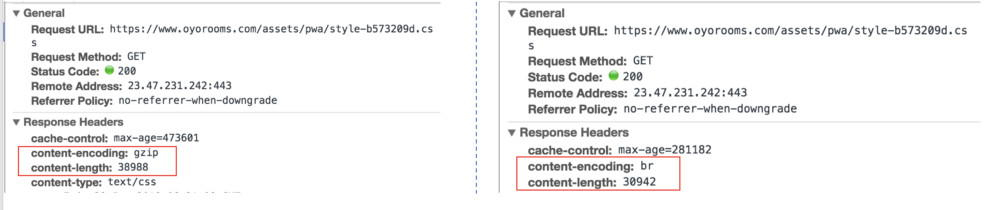
\includegraphics[width=0.95\textwidth]{images/header.png}
\caption{Comparção entre os \textit{headers} HTTP GZIP e Brotli\cite{headerImage}}\label{packet123}
\end{figure}


\subsection{Compressão de imagens}\label{compressimaage}

\par As imagens são um ponto importante dos sistemas IOT, onde o utilizador através de esquemas, imagens e gráficos consegue obter o que pretende sem muito esforço. O sistema Nidus apenas despõe de imagens em algumas versões a pedido de clientes devido ao sobre carregamento de espaço que acarreta a utilização de imagens.
\par Para desenvolver uma interface com recurso a sistemas visuais é necessário ter ou uma imagem com uma qualidade estipulada para o ecrã máximo necessário para ser possível reduzir a mesma em ecrãs mais pequenos, ou existirem múltiplas imagens de vários tamanhos para cada tipo de ecrã. A utilização de imagens pequenas que ocupem pouco espaço em disco, aquando da utilização em ecrãs maiores irá provocar visível na imagem cada pixel revelando ao utilizador a fraca qualidade do sistema. Na utilização de imagens superior ao máximo dos ecrãs e fazer o redimensionamento para um tamanho inferior, torna as imagens mais atrativas, pois o efeito não provoca o aparecimento da imagem “Pixelizada”. Isto implica mais espaço de memória para alojar imagens, que não existe na configuração de \textit{hardware} atual do sistema Nidus. Em alternativa às codificações mais comuns nas imagens (PNG, JPEG, entre outras) existe a possibilidade de em imagens que não representem fotografias a utilização de SVG. No SVG ao contrário dos outros formatos indicados não é feita a representação de cada pixel da imagem, mas sim a definição de uma função que representa uma reta, uma forma, um polígono, ou as coordenadas de pontos, sobre a forma de uma estrutura XML. O HTML já possui suporte  para elementos SVG, Na utilização de SVG dentro de páginas HTML é possível a utilização de todas as funcionalidades inerentes ao CSS tais como criar animações. 
\par Outra funcionalidade possível com a utilização de SVG é a alteração do texto existente na imagem apenas fazendo a alteração do valor do elemento XML, à semelhança da alteração do texto numa página HTML.

\par Os editores de SVG possuem variadas opções que não representam nada para o utilizador final, são apenas informações para o próprio editor. Para remover essa informação são utilizadas ferramentas para a remoção de tal informação. A ferramenta escolhida durante o estágio foi a SVGO\cite{svgo}, uma ferramenta desenvolvida em node.js de modo a otimizar os SVG. Com esta ferramenta é possível remover toda a informação desnecessária e otimizar e simplificar algumas funções não afetando a qualidade da imagem. De modo a ser possível em tempo real fazer alterações é necessário á semelhança das páginas HTML cada elemento possuir um ID para fazer a sua procura na árvore XML e deste modo ser possível alterar a cor, o conteúdo do texto adicionar animações. O próprio SVG possibilita a inserção de imagens PNG, JPEG dentro do SVG. Estas imagens são adicionadas ao XML sob a forma de Base64. No apêndice \ref{svg} é apresentado o exemplo do svg gerado pelo editor. No Apêndice \ref{svggo} a respetiva compressão utilizando a ferramenta SVGO. Uma das considerações na utilização do SVGO é a necessidade de preservar os ID's e não os remover durante a compressão. Para tal na utilização da ferramenta é necessário indicar que  pretendemos manter os ID's, para tal basta durante a utilização utilizar a opção '--disable=cleanupIDs'.

\par Para criar animações á semelhança do HTML é possível atribuir classes a cada elemento do SVG e tirar partido das animações possíveis no CSS. 
\par No gráfico da figura \ref{compSV} é apresentado o tamanho ganho na compressão do SVG do Apêndice \ref{svg}. O Tamanho do SVG após a otimização com a ferramenta SVGO é de apenas cerca de 20\% do tamanho original (2 485b - 80\%= 559b).

\begin{figure}[ht]
\centering
\begin{tikzpicture}
\begin{axis}[
xbar,
height=5cm,width=10.8cm, 
y axis line style = { opacity = 0 },
axis x line = none,
tickwidth = 0pt,
enlarge y limits = 0.7, 
enlarge x limits = 0.02,
symbolic y coords = {Original, Otimizado},
nodes near coords,
ytick=data,
legend style={
at={(rel axis cs:0.5,1)},
anchor=south,
legend columns=-1, 
column sep=2mm, 
draw=none 
}
]
\addplot coordinates { (2485,Original) (559,Otimizado) };
\legend{SVG- Apêndice \ref{svg}}
\end{axis}
\end{tikzpicture}

\caption{Gráfico com comparação do tamanho entre original e otimizado(em Bytes)}\label{compSV}


\end{figure}

\subsection{Desenvolvimento a pedido de cliente}

\par Durante o estágio existiu apenas um desenvolvimento pedido pelo cliente. O cliente pretende utilizar uma Nidus IT para controlar o seu sistema de alimentação dos animais de forma automática. Além de todas as questões a tratar no Back-end da Nidus, relativas a funcionamentos específicos da solução, o cliente pretende aceder na página da Nidus uma interface visual para inserir num monitor com o estado da alimentação, dos motores, da água. Este desenvolvimento para a sua realização usou as capacidades referidas no capítulo \ref{compressimaage}, de modo para obter uma imagem única e responsiva com animações em tempo real. Após o desenho da interface pretendida no editor SVG, o mesmo foi comprimido com a ferramenta SVGO indicada anteriormente. \par De modo a criar uma interface atrativa ao utilizador foram criadas algumas animações nos sem fins da alimentação, no silo da alimentação indicando o seu estado atual, tal como o estado das condutas de água.

\begin{figure}[ht]
\centering
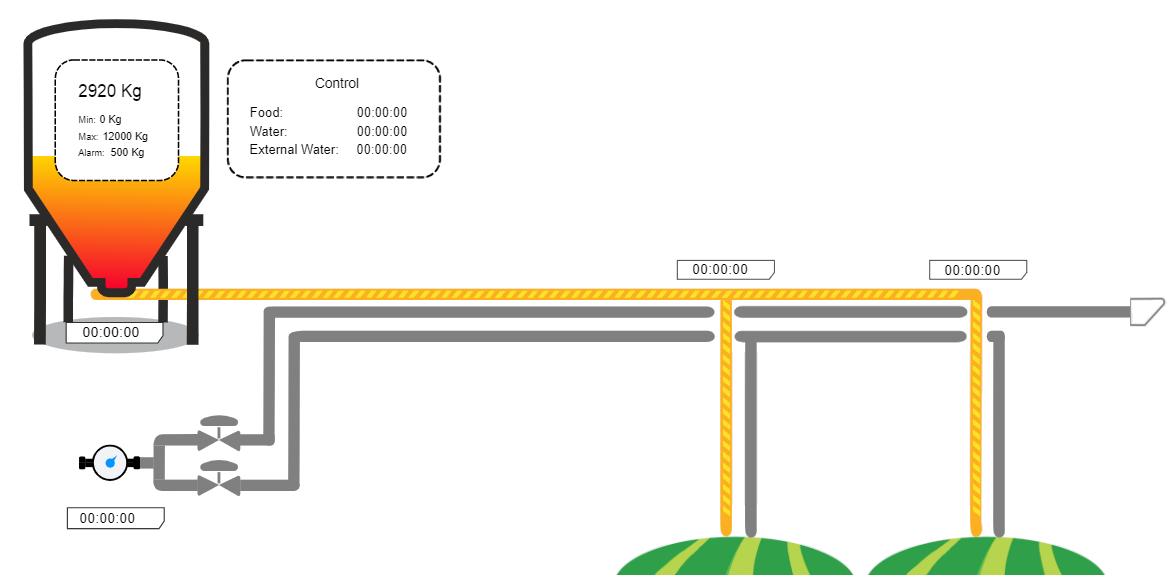
\includegraphics[width=0.95\textwidth]{images/svgpig.png}
\caption{Exemplo do SVG utilizado na Solução}\label{pig}
\end{figure}

\subsection{Correção de \textit{bugs}}

\par Durante o estágio apenas foi reportado a existência de um \textit{bug}. Estre prede-se com a estrutura criada para comunicação entre o \textit{Front-end} e o \textit{Back-end} ou com sistemas que pretendam integrar os equipamentos Nidus.
\par No momento do carregamento da página WEB, a mesma solicita um ficheiro XML com todas as informações necessárias. Em alguns dos pontos da estrutura como por exemplo o caso dos Input, Outputs, Sensores, entre outros, os mesmos são agrupados num elemento principal como é possível observar no exemplo seguinte.

\begin{verbatim}
1 ...
2 <Sensors>
3     <Entry>
4         <ID>0</ID>
5 ....
6     </Entry>
7     <Entry>
8         <ID>1</ID>
9 ....
10    </Entry>
11 ...
12 </Sensors>

\end{verbatim}



\par Este ID é utilizado na comunicação de modo a indicar a que sensor se refere os dados. O problema surge aquando da eliminação de um sensor. Supondo o seguinte cenário. É eliminado o sensor com o ID 0, o sistema Nidus eliminar o sensor e a entrada no XML com o ID 0 fica inutilizada passado o XML a conter os ID's 1,2,3,4 ,... de modo ao sistemas que integram a Nidus poderem utilizar o ID como uma chave primária. O problema reside no código JavaScript que converte o XML numa variável JavaScript, mais concretamente num \textit{array}. O sistema em alguns dos pontos do código ao invés de utilizar o valor presente no elemento ID, utilizava a sua posição no \textit{array}, fazendo que em sistemas onde tivessem sido feitas alterações (Exemplo: eliminar sensores) os ID's não correspondiam. Supondo o exemplo seguinte onde existem dois sensores com os ID's 0 e 1. Na conversão para um objeto no JavaScript era obtida a estrutura apresentada na figura \ref{estruct1}.

\begin{verbatim}
1 ...
2 <Sensors>
3     <Entry>
4         <ID>0</ID>
5         <Name>0</Name>
6     </Entry>
7     <Entry>
8         <ID>1</ID>
9         <Name>1</Name>
10     </Entry>
11 ...
12 </Sensors>

\end{verbatim}

\begin{figure}[ht]
\centering
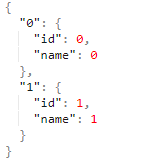
\includegraphics[width=0.25\textwidth]{images/estructu1.png}
\caption{Estrutura obtida no JavaScript - 1}\label{estruct1}
\end{figure}

\par Após a eliminação do Sensor 0, o XML obtido é similar ao apresentado de seguida. Neste caso o \textit{array} criado no JavaScript era similar ao apresentado na figura \ref{estruct2}. O problema reside na utilização da posição do \textit{array} em algumas partes do código nomeadamente na procura do sensor. No exemplo apresentado na figura \ref{estruct2} antes da correção do \textit{bug} o código existente ao necessitar dos dados do sensor com o ID 1 aceder á posição 1 do \textit{array}, ao invés de procurar por cada elemento qual o elemento que possui aquele id. 
\par No caso de terem sido eliminados alguns sensores como apresentado neste exemplo os dados selecionados não correspondem ao pretendido pelo utilizador.

\begin{verbatim}
1 ...
2 <Sensors>
3     <Entry>
4         <ID>1</ID>
5         <Name>1</Name>
6     </Entry>
7     <Entry>
8         <ID>2</ID>
9         <Name>2</Name>
10    </Entry>
11 ...
12 </Sensors>

\end{verbatim}

\begin{figure}[ht]
\centering
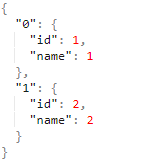
\includegraphics[width=0.25\textwidth]{images/estruct2.png}
\caption{Estrutura obtida no JavaScript - 2}\label{estruct2}
\end{figure}


\par De modo a resolver o problema identificado foi criada no projeto uma função com 3 parâmetros. No primeiro parâmetro é indicado o \textit{array} onde deve o sistema procurar. Em seguida é indicado em que propriedade pretendemos compara e por último indicamos o valor que pretendemos encontrar. No código seguinte é apresentado o código utilizado. Caso o elemento não exista é devolvido o valor \textit{null}.
\begin{verbatim}
1 function findObjectByKey(array, key, value) {
2     for (var i = 0; i < array.length; i++) {
3         if (array[i][key].toString() === value.toString()) {
4             return array[i];
5         }
6     }
7     return null;
8 }
\end{verbatim}

\par Ao invés do acesso á posição diretamente no \textit{array} é necessário a alteração de todo o código para fazer utilização da função e obter o valor correto.
\subsection{Melhoramento da página}
\par Após análise prévia da página do sistema Nidus, foi acordado a necessidade de desenvolver um sistema mais simplificado para o processo de criação de eventos. Pretende-se assim estudar a melhor solução para a criação das ações e das reações e uma interface para criar os eventos com recurso às ações e reações previamente criadas. Todas as opções e menus para a criação e manutenção das ações e reações mantém-se inalteradas no momento atual. Já a criação de eventos necessita de ser restruturado, após debate chegou-se á decisão de necessitar de um sistema visual onde o utilizador por blocos é capaz de criar a situação que pretende.
\par Durante o estágio foram analisadas as opções possíveis para a solução pretendida. Após análise foi adotado a utilização do plugin Blockly\cite{blockly}, devido á sua semelhança com o pretendido (Scratch) e devido ao baixo espaço ocupado pós compressão e á possibilidade de criar os próprios tipos de blocos. Devido aos restantes projetos realizados durante o estágio este desenvolvimento ainda não se encontra concretizado e apenas foi selecionado a solução a adotar. No gráfico da Figura \ref{block} é apresentado o espaço ocupado pelo código fonte do \textit{plugin} escolhido.


\begin{figure}[ht]
\centering
\begin{tikzpicture}
\begin{axis}[
xbar,
height=5cm,width=10.8cm, 
y axis line style = { opacity = 0 },
axis x line = none,
tickwidth = 0pt,
enlarge y limits = 0.7, 
enlarge x limits = 0.02,
symbolic y coords = {Minificado, GZIP},
nodes near coords,
ytick=data,
legend style={
at={(rel axis cs:0.5,1)},
anchor=south,
legend columns=-1, 
column sep=2mm, 
draw=none 
}
]
\addplot coordinates { (76455,Minificado) (13456,GZIP) };
\legend{Blockly}
\end{axis}
\end{tikzpicture}

\caption{Gráfico com comparação do tamanho do plugin Blockly (em Bytes)}\label{block}


\end{figure}



\section {NB-Iot \& Digi Xbee 3 }
\par
O desenvolvimento do projeto NB-Iot \& Digi Xbee 3 é composto por 4 fases, 3 das quais desenvolvidas durante este estágio. A fase não desenvolvida durante o estágio refere-se ao desenho e produção do \textit{hardware} e a parte do \textit{software} referente á leitura de sensores (comunicação entre \textit{hardware} desenvolvido e \textit{software}). As fases realizadas durante o estágio são a implementação do envio do pacote definido com os mecanismos de proteção e segurança, sincronismo dos tempos de leitura e envio e testes ao sistema.

\subsection {Envio de dados para o portal}

\par Como foi indicado no Capítulo \ref{nbiot} a estrutura de pacote a enviar é similar ao do outro produto desenvolvido pela Captemp. Este pacote é enviado através de um pacote UDP para o portal que posteriormente confirma a receção na camada de aplicação. O tamanho máximo definido para este pacote é de 1000 bytes.
A estrutura criada pela Captemp segue o formato apresentado na figura \ref{packet}.
\par No primeiro cabeçalho é possível obter os dados do equipamento que fez o envio tais como a data de envio, o IMEI, a versão do mesmo e o CRC do pacote para confirmar a integridade do mesmo. No restante do pacote são adicionados vários sub pacotes seguindo a estrutura apresentada na figura \ref {packet}, o primeiro byte indica o tipo de dados se é envio o valor de um sensor uma configuração do equipamento(Exemplo: Operadora), o byte seguinte fornece o número de bytes dos dados e posteriormente segundo o número de bytes, o valor (Exemplo: operadora ="ALTICE").

\begin{figure}[ht]
\centering
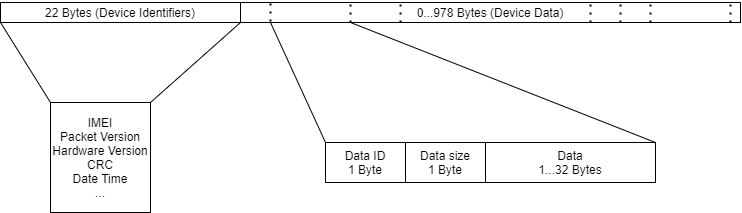
\includegraphics[width=0.95\textwidth]{images/packetnb.png}
\caption{Estrutura do Pacote NB-IOT}\label{packet}
\end{figure}

\subsection {Gestão de memória}

\par O principal motivo da desistência da utilização deste equipamento como o equipamento principal da Captemp para o NB-Iot prendeu-se com a incorreta gestão de memória do MicroPython. Segundo a documentação quando uma variável já não é acessível pelo código esta é removida pelo \textit{Garbage Collector} mas o espaço de memória ocupado fica disponível e nem todas as vezes é utilizada pelo MicroPython e este aloca no final ao invés de procurar o primeiro espaço disponível. No esquema apresentado na figura \ref{memo} é apresentado o comportamento da memória com a gestão nativa do MicroPython, com o decorrer do tempo a memória fica totalmente alocada não permitindo ao equipamento guardar novas leituras nem enviar para o portal.


\begin{figure}[ht]
\centering
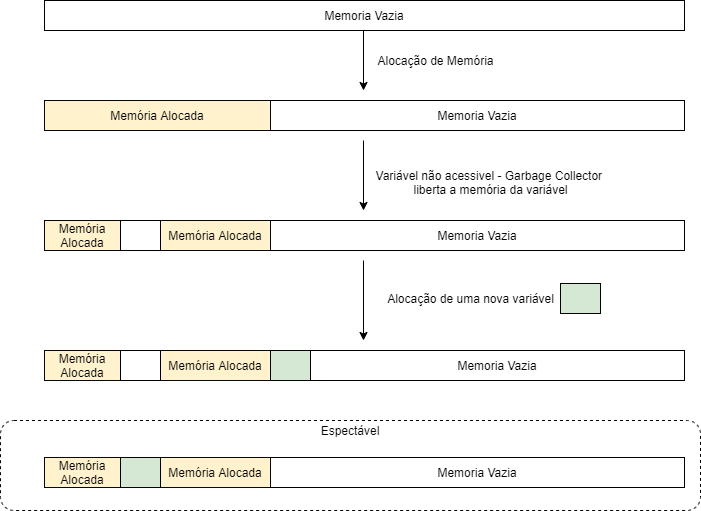
\includegraphics[width=0.90\textwidth]{images/memo.png}
\caption{Comportamento da gestão de Memória}\label{memo}
\end{figure}



\subsubsection {Diminuição da alocação de memória}

\par A modo de resolver a incorreta gestão de memória é necessário diminuir a alocação de novas variáveis. Para tal todo o código do programa visa a possuir todas as constantes e variáveis em variáveis globais as quais nunca são eliminadas e criadas apenas alteram o seu valor. Os dois pontos críticos identificados são o \textit{array } circular com as leituras dos sensores e a criação do pacote de envio para o portal \textit{Cloud}.
\par Na criação do pacote todos os cabeçalhos fixos são alocados em constantes globais que não vem o seu valor alterado não afetando a memória e os valores que podem ser alterados são guardados em \textit{buffers} globais criados no inicio e tem o seu tamanho estático. Devido á utilização de um módulo que não possui suporte para \textit{multri thread} não existe problema de sincronismo entre os fluxos ao utilizar as variáveis e os \textit{buffers} globais. Ao recolher um dado de modo a enviar para o portal, como por exemplo a operadora, este tem de ser alocado num \textit{buffer} que depois é enviado pela rede para o servidor. Este \textit{buffer} de bytes com o tamanho fixo do máximo do pacote de envio é utilizado para fazer a concatenação dos vários campos antes do envio ao invés da abordagem anterior da utilização de um \textit{buffer} de tamanho dinâmico. Caso se pretenda adicionar valores a enviar é consultada o ultimo \textit{byte} ocupado, encontrada numa variável separada e é alterado os bytes das posições seguintes para o bytes do valor não alocando memória para continuar o \textit{array}.
\par Supondo que o \textit{buffer} tem já preenchidos 300 bytes dos 1000, ao pretender adicionar o pacote da operadora, é copiado para a posição 301 o byte correspondente ao DATA ID do operador, no byte seguinte é colocado o tamanho de bytes que a operadora ocupa ("ALTICE"= 6 Bytes), e nos seguintes 6 bytes é colocada a \textit{string}.
\par No exemplo acima elucidado todas as variáveis são estáticas, o DATA ID é definida no inicio do código, o tamanho foi previamente guardado numa variável auxiliar de tamanho fixo, e a operadora é solicitada a funções nativas do MicroPtyhon e guardado num \textit{buffer} de tamanho fixo. Após a definição apenas são efetuadas copias de bytes entre variáveis e \textit{buffers} não afetando a alocação de memória. No código seguinte é exemplificado a operação anteriormente apresentada. Neste caso de modo a simplificar é apresentado um \textit{buffer} do tamanho da operadora, no projeto foram criados \textit{buffers} do tamanho 1,2,4,10,16,32 bytes consoante os valores mais comuns, no caso particular de um valor dinâmico que possa ter por exemplo 20 bytes este é guardado no \textit{buffer} de 32 e no momento da gravação apenas são copiados os 20 primeiros bytes.

\begin{verbatim}
1  c=bytearray(1000) # Packet Array
2  clean=bytearray(1000) # Empty Packet Array 
3 
4  #BUFFERs
5 
6  cmd6=bytes(6)
7  cmdID=bytes(1)
8  cmdLEN=bytes(1)
9 
10 #DATA IDs
11 c0=bytes([0x01])
12
13  (...) 
14
15 cmdID = c0 # DATA ID
16 cmdLEN = (6).to_bytes(1, 'little') # Data Size
17 cmd6 = bytes(oper, 'ascii') # Data (string to bytes)
18 byteschange(c, 300, 301, cmdID) # Copy to packet array 
19 byteschange(c, 301, 302, cmdLEN) # Copy to packet array 
20 byteschange(c, 302, 308, cmd6) # Copy to packet array 
\end{verbatim}

\par Ao copiar valores de entre \textit{buffers} e não alocando espaço ao \textit{array}, é necessário um maior controlo nos tamanhos das variáveis de modo a não copiar valores de \textit{buffers} vazios ou posições inexistentes. A versão do MicroPython disponibilizada pela Digi não incorpora a biblioteca que faz a gestão de \textit{arrays} limitando não possibilitando a copia direta de \textit{arrays} para outros \textit{arrays} indicando apenas a posição inicial. Para tal a função desenvolvida, byteschange utilizada previamente no código, simula essa operação onde apenas indicamos o \textit{buffer} de destino, a posição inicial, a final e a origem da cópia. Esta função é responsável por verificar se os tamanhos são possíveis de copiar e copia posição a posição (byte a byte no caso apresentado) para as posições entre os valores indicados. No fim do pacote ser enviado é possível limpar o \textit{buffer} chamando a mesma função indicando como origem da copia o \textit{buffer clean}, um \textit{buffer} constante do mesmo tamanho mas com os bytes todos vazios. Todos os \textit{buffers} utilizados ao longo do projeto tem um semelhante em tamanho, mas completamente vazio. Deste modo é possível utilizar sempre os mesmos \textit{buffer} e não existir a necessidade de alocar \textit{buffer} ao longo do programa.

\subsubsection {Gestão da memória durante leituras}

\par À semelhança do \textit{buffer} onde é gerado o pacote enviado para o portal, as leituras são um dos pontos críticos referente á alocação de memória. Para tal á semelhança do pacote de envio, é inicializado no início do programa, um \textit{array} de tamanho fixo e com cada posição com um \textit{array} do tamanho máximo ocupado por uma leitura com o máximo de sensores do equipamento. Ao adicionar uma nova leitura são colocados nos \textit{buffers} intermédios todos os dados e são copiados para a posição seguinte á última posição ocupada. Caso a última posição ocupada corresponda à última do \textit{array}, é adicionado sobre a primeira posição, criando assim o \textit{array} circular.
\par Todas as operações para adicionar uma leitura ao \textit{array} ou remover são efetuadas com a função byteschange de copiando o \textit{buffer} temporário com a leitura ou o vazio respetivamente. Na figura \ref{circbuf} é apresentado o esquema do \textit{array} circular com as leituras. Como \textit{array} é definido inicialmente e o utilizador pode alterar as sondas enquanto o equipamento está em funcionamento é sempre alocado para cada leitura o numero de bytes necessário para o máximo de sensores garantindo que caso o utilizador adicione um sensor não seja necessário expandir o tamanho da posição no \textit{array} causando os problemas de memoria já identificados. Para eliminar uma leitura é decrementado a posição corrente do \textit{array} e por proteção de modo a posteriormente não acedermos a dados que possam lá existir, como por exemplo numa leitura antiga com 6 sensores e nova com 3 sensores os últimos 3 sensores da leitura antiga ainda estavam associados apesar de no cabeçalho da leitura indicar que são apenas 3, é copiada a leitura vazia para a posição da leitura garantimos que não existem dados sem nexo a afetar alguma das leituras.


\begin{figure}[ht]
\centering
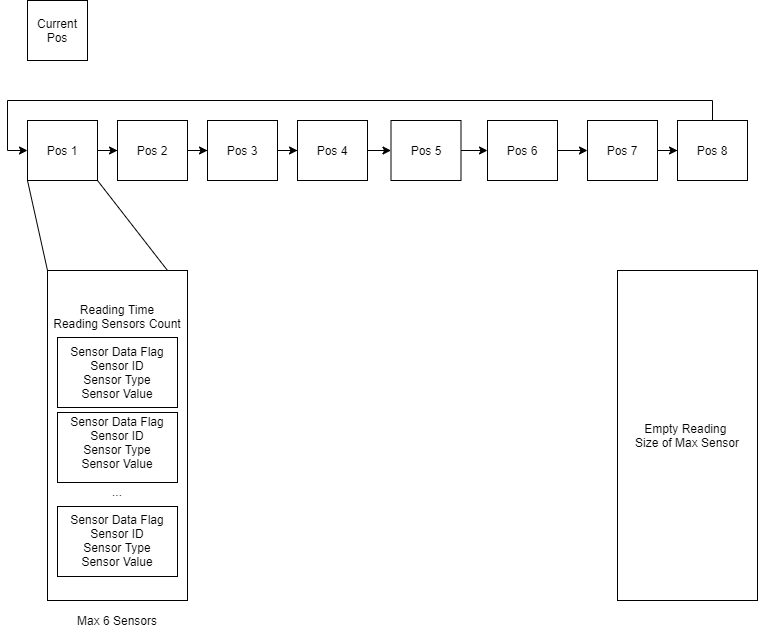
\includegraphics[width=0.85\textwidth]{images/circbuf.png}
\caption{Array Circular com leituras}\label{circbuf}
\end{figure}

\subsection {Sincronismo de leitura e envio} \label{sinc}

\par À semelhança dos restantes produtos produzidos pela Captemp existe sempre sincronismo de leituras entre os equipamentos. Para tal além de cada equipamento possuir um relógio interno (RTC), é necessário fazer o sincronismo na primeira leitura, ou seja caso esteja programado para fazer a leitura a cada 5 minutos, existe uma diferença caso o mesmo seja ligado ás 00:00 e fazer as leituras respetivamente às 00:05, 00:10,00:15,00:20 , mas caso seja ligado por exemplo às 00:12, faz leituras às 00:17,00:00:22 e por diante não existindo um sincronismo entre os vários equipamentos dos clientes.
\par Para tal o equipamento no momento inicial do arranque verifica qual o intervalo de leitura e de envio, e verifica caso fosse ligado pelas 00:00 qual seria a próxima leitura ao momento atual, neste momento o equipamento não entra em modo de poupança de energia durante os 5 minutos até á leitura e apenas o tempo restante até ao valor caso fosse ligado pelas 00:00, no momento da leitura o equipamento já entra em modo de poupança de energia durante o tempo definido (Ex:5 minutos). Este método é igualmente aplicado ao intervalo de envio. Aquando do envio é enviado na resposta proveniente do servidor o \textit{Timestamp} do servidor de modo a sincronizar o tempo de todos os equipamentos e configurar nos novos equipamentos que sejam ligados e ainda possuam o valor \textit{default} do RTC, no caso do escolhido no projeto 1 de Janeiro de 2000.
\par Caso o equipamento possuir uma data inferior á estipulada de 1 de Janeiro de 2019, o mesmo não faz leituras, esperando pelo intervalo de envio para enviar um pacote apenas com os campos fixos e sem leituras de modo a obter a resposta com o \textit{timestamp} do servidor para iniciar as leituras.


\subsection {Encriptação dos dados}

\par De modo a proteger os dados na rede todo o pacote é encriptado com recurso á biblioteca MicroPython-AES disponibilizada \textit{online} \cite{microaes}. Esta biblioteca desenvolvida para o MicroPython Base e não para a versão disponibilizada nos módulos DIGI, é necessário reformular a biblioteca de modo a não utilizar a biblioteca de gestão de \textit{arrays} indisponível nesta versão e fazer a alteração aquando da necessidade de acrescentar dados no \textit{array} colocar posição por posição. No código seguinte é apresentado o problema inerente a esta biblioteca (linha 4) e a sua respetiva resolução (linha 13).


\begin{verbatim}
1   for offset in range(0, len(data), block_size):
2       block = data[offset:offset + block_size]
3       block_func(block)
4       data[offset:offset + block_size] = block # ERROR 
5       #['array' object does not support item assignment]
6  ...
7
8  ...
9   for offset in range(0, len(data), block_size):
10     block = data[offset:offset + block_size]
11     block_func(block)
12     # Solution ['array' object does not support item assignment]
13     for i in range(block_size)
14         data[offset+i]= block[i]
15 ...
\end{verbatim}

\section {Kea Tracker}

\par De modo a substituir um produto descontinuado e apresentar novas soluções aos clientes, irão ser utilizadas beacons para armazenar os valores da temperatura, humidade e pressão ambiental para posterior envio para o portal Senslive. No início do estágio não estava disponível nenhuma versão de \textit{Firmware} com armazenamento dos dados e estava proposto o desenvolvimento da solução utilizando o Espruino, uma plataforma que permite fazer a programação de microcontroladores com recurso a JavaScript. Foram realizados pequenos testes e chegou-se á conclusão que a camada interpretadora do Javascript tem um consumo mais elevado comparando com uma versão desenvolvida em C. Além do maior consumo energético, já foi disponibilizado um \textit{Firmware} com armazenamento de leituras para posterior arquivo. Devido a esses dois fatores não será desenvolvido o \textit{Firmware} como estava inicialmente proposto e irá ser apostado no melhoramento e desenvolvimento da aplicação responsável por obter os dados e enviar para o portal Senslive. 


\subsection{App - Alterarações necessárias}

\par A aplicação na primeira fase irá ser baseada na fornecida pela Ruuvi e serão alteradas as referências referentes ao \textit{website} da RuuviTag para o \textit{website} da Captemp e a alteração das imagens para o novo logótipo da solução. Devido é necessidade de desenvolvimento do \textit{Back-end} no Senslive, será desenvolvida apenas adaptada a versão Android, e na segunda fase do projeto desenvolvimento de uma versão Android e IOS com recurso a uma plataforma que permita o desenvolvimento para ambas as plataformas com apenas um código fonte, tais como o NativeScript\cite{nativescript}, o Ionic\cite{ionic} entre outras.

\subsection{App - Novas funcionalidades}

\par A aplicação fornecida pela Ruuvi não está desenvolvida para a leitura das leituras quando a beacon não esteve ao alcance. É necessário então desenvolver o módulo por obter essas leituras e guardar na base de dados para a restante aplicação enviar para o portal Senslive.
\par O \textit{Firmware} disponibilizado converte a RuuviTag numa beacon connectável e disponibiliza sobre a forma de um serviço os Logs da mesma\cite{ruuvitlog}. Para tal é necessário adaptar a aplicação de modo a quando esta esteja encontra uma nova beacons ao alcance descarregue o seu Log. Quando a beacon se encontra sempre ao alcance a aplicação não necessita de fazer a conexão para descarregar os Logs visto esta além da conexão faz o \textit{broadcast} dos dados em tempo real. O principal problema a resolver neste projeto é o sincronismo de leituras, já retratado no capítulo \ref{sinc} quando a aplicação se encontra a registar através do \textit{broadcast}. Nos Logs não é possível fazer esse sincronismo devido á mesma não possuir essa funcionalidade internamente. No \textit{download} dos Logs é necessário verificar quais as leituras de Log que possam ser referentes a intervalos que existiu a receção de \textit{broadcast} e tiveram leituras sincronizada, não sendo necessário o armazenamento. É espectável com o \textit{Firmware} selecionado obter uma autonomia entre 2 a 3 anos com ligações esporádicas para descarregar Logs ou 6 meses com a conexão sempre ativa. No Fluxograma do apêndice \ref{E} é possível observar o ciclo referente á obtenção das leituras e dos Logs.


% O principal problema deste projeto a resolver é a definição do intervalo que a aplicação deve descarregars os Logs da Beacon. No caso mais simples a aplicação num intervalo programado e fixo descarrega os Logs desde o ultimo \textit{download}, mas é criado um problema caso a beacon não esteja ao alcance no preciso momento do intervalo. Caso falhe um intervalo a beacon tem suporte para no intervalo seguinte descarregar ambos os intervalos, mas tem um limite, este variável consoante o valor definido como intervalo de \textit{download}. No caso apresentado anteriormente, no momento definido para descarregar os Logs a beacon pode não estar ao alcance, mas a mesma pode ter estado ao alcence momento antes ou momentos futuros. Nesses casos a aplicação deve segundo o tempo desde a ultima conecção verificar se a deve se ligar a beacon ou não diminuindo a possibilidade de perder leituras. Esta solução é necessário pois a beacon com o \textit{firmware} em questão caso esteja sempre com a connexão ativa para descarregar o Log da última leitura apenas tem autonomia para 6 meses e caso seja feito o \textit{download} periodicamente de um conjunto de Logs, uma autonomia espectável entre 2 e 3 anos. 

\subsubsection{\textit{Download} manual}
\par A aplicação desenvolvida permitirá ainda ao utilizador a possibilidade de fazer um \textit{download} manualmente, configurar o máximo de tentativas do \textit{download} automático, com o valor de \textit{default} definido em 1. Além dessa configuração é implementada uma medida de segurança onde caso o RSSI seja inferior a -90, significando que se encontra longe não são descarregados os Logs devido á possibilidade de perder a ligação no \textit{download}, neste caso é apresentado ao utilizador uma nota para aproximar o equipamento da beacon. %Caso uma das beacons entre no alcance do Smartphone e a mesma tenha estabelecido a última ligação num intervalo superior ao configurado(\textit{default}- 1 Hora) a aplicação estabelecerá automaticamente a ligação para descarregar e minimizar a perda de leituras. Igualmente caso a beacon antes do intervalo definido esteja ao alcance e o sinal tenha um valor baixo, significando que se encontra longe e poderá não conseguir descarregar os dados a app descarrega os dados minimizando igualmente as perdas de possíveis dados.

\subsection{Desenvolvimento de uma aplicação multi-plataforma}

\par A \textit{Framework} escolhida foi o Ionic, uma \textit{Framework open-source} que permite o desenvolvimento de aplicações \textit{mobile} para múltiplas plataformas com o mesmo código, melhorando o tempo necessário para o desenvolvimento e simplificando os processos de atualização visto apenas existir um código fonte a atualizar. 
\par Esta fase do projeto Kea.Tracker é referente á conversão da aplicação existente em Kotlin para o Ionic e migrar todas a funcionalidades existentes atualmente na versão em Kotlin. 
Ao invés da utilização de \textit{Activities} como no Kotlin o Ionic utiliza um sistema similar a um serviço WEB onde são criadas várias rotas e é possível navegar entre elas. Todo o \textit{design} da platadorma seguiu o mesmo layout da aplicação já existente, onde foram retiradas as opções de alertas e vizualização dos gráficos visto pretendermos centralizar essas opões no portal Senslive e utilizar a aplicação apenas como um \textit{Gateway}. Fica assim disponível na aplicação apenas de adicionar novos equipamentos ao gateway neste caso a App, editar o nome do equipamento para mais fácil distinção entre os vários equipamentos, as configurações da aplicação e um serviço em \textit{Background} para realizar as leituras sem necessidade da aplicção estar aberta.
	
\subsubsection{Distinção entre \textit{Beacons} \& Leitura de Dados  }

\par Para facilitar a utilização da interface da aplicação ao utilizador da mesma ao adicionar um novo dispositivo apenas são mostrados os dispositivos ao alcance que correspondam a equipamentos da Ruuvi que estejam a transmitir os dados nos formatos definidos. Todos os equipamentos BLE nos dados transmitidos em \textit{Broadcast} possuem informaçãoes no \textit{header} da transmissão, tais como o fabricante, denominado de \textit{"Company Identifier"}. No caso das \textit{Beacons} da Ruuvi é enviado o código  correspondente á Ruuvi, "0x0499. Estes códigos podem ser consultados na documentação do \textit{Bluetooth} \cite{companySI}. Juntamente com o \textit{Company Identifier} o protocolo define mais alguns parâmteros tais como o tamanho do header. No caso das \textit{Beacons} da Ruuvi é enviado os dados referentes aos sensores nos diversos formatos definidos na documentaão da Ruuvi \cite{GitHubRuuvi}, precedidos por um byte com o valor correspondente  ao formato dos dados.
\par Segundo a documentação a aplicação deve suportar a leitura em tempo real de dois formato o formato 3 e 5, pois são estes os existentes nas \textit{Beacons} atuais



\section {dot.Tracker}
\par
A pedido de um cliente, foi proposto o desenvolvimento de uma plataforma WEB para fazer a monitorização de pessoas e objetos em tempo real. O projeto passou por várias etapas das quais destacam-se a análise dos requisitos do cliente, análise de tecnologias disponíveis, análise de soluções existentes já em comercialização, o desenvolvimento do portal Web, desenvolvimento do Back-End, e testes ao sistema. Apesar do projeto ser apenas desenvolvido por um elemento, mas devido á maior complexidade e duração do mesmo foi adotada a metodologia SCRUM com entregas/apresentações ao cliente para obter o \textit{feedback} do trabalho desenvolvido e assim poder alterar alguns dos requisitos solicitados.
\par O Cliente indicou que devia ter atualizações dos mapas em tempo real, alertas enviados para o cliente WEB caso este esteja \textit{online} e por email.
É assim possível definir a tabela, apresentada na tabela \ref{tab1} com os requisitos da solução e a sua importância no desenvolvimento.

\begin{table}[htb]
\centering
\caption{Requesitos da solução}\label{tab1}
\begin{tabular}{|p{3cm}|p{8cm}|p{2cm}|}\hline
Requesito&Descrição&Importância (1-10)\\\hline

Portal Cloud (Front-End)&Portal Cloud com mapas em tempo Real& 7\\\hline
Portal Cloud (Back-End) & API REST para integração com o Front-End e recolha dos dados para a localização &9\\\hline
Histórico de posições&Possibilidade de re-visualizar no mapa o percurso entre datas&5\\\hline
Alertas Email&Alertas de Email (Exemplo: Entrada e Saída de zonas criadas no mapa )&6\\\hline
Alertas Web&Alertas Informativos no Mapa (Exemplo: Entrada e Saída de zonas criadas no mapa )&2\\\hline
\end{tabular} 
\end{table}

\par
De seguida são apresentados as funcionalidades e objetivos de cada requisito e escolhas selecionadas.

\subsection {Portal Cloud - \textit{Front-End}}

\par O \textit{Front-end} da solução é desenvolvido com recurso á \textit{Framework Vue}, tornando a solução numa solução \textit{Single-Page Aplication}. A adoção da \textit{framework} é baseada na necessidade de possuir fluidez na navegação entre páginas e igualmente nos mapas em tempo real minimizando o \textit{delay}.
\par A plataforma é capaz igualmente de suportar várias \textit{Companies}, significa isto que é possível criar várias \textit{Companies} e temos os administradores e os utilizadores normais de cada \textit{Company} que apenas tem acesso ás suas definições e equipamentos. Possibilitando fornecer o projeto como uma solução \textit{Cloud} a váriados clientes no mesmo servidor, onde cada um apenas possui o acesso ao que pertence à sua \textit{Company}.
No final o utilizador da plataforma deve ser capaz de realizar as seguintes operações:
\par
\begin{itemize}
\item Login na plataforma para visualizar os dados
\item Visualizar mapas com atualizações em tempo real
\item Editar o seu perfil
\item Visualizar a página numa língua á sua escolha
\item Utilizar a plataforma em vários equipamentos PC, Tablet, Smartphone,...
\item Gerir utilizadores (Administradores)
\item Gerir equipamentos (Administradores)
\item Gerir mapas e zonas (Administradores)
\item Gerir alertas (Administradores)
\item Iniciar/ finalizar missões (Administradores)
\end{itemize}


\subsubsection{\textit{Login}}
\par Para aceder á plataforma é necessário aos utilizadores procederem ao login na mesma, uma vez que possuímos uma API o \textit{login} é realizado através de Json WebTokens ou simplesmente, JWT. No momento do \textit{login} são enviadas as credenciais para o servidor, caso este as valide cria um \textit{Token} que é devolvido ao cliente e este em futuras requisições à API inclui o \textit{token} identificando-se e autenticando-se perante o servidor. Este método de login é regularmente utilizado devido á necessidade de possuir métodos \textit{stateless} ao invés da utilização de variáveis de sessão. No exemplo apresentado na figura \ref{jwt1} é apresentado o conteúdo de um textit{Token} JWT. 


\begin{figure}[ht]
\centering
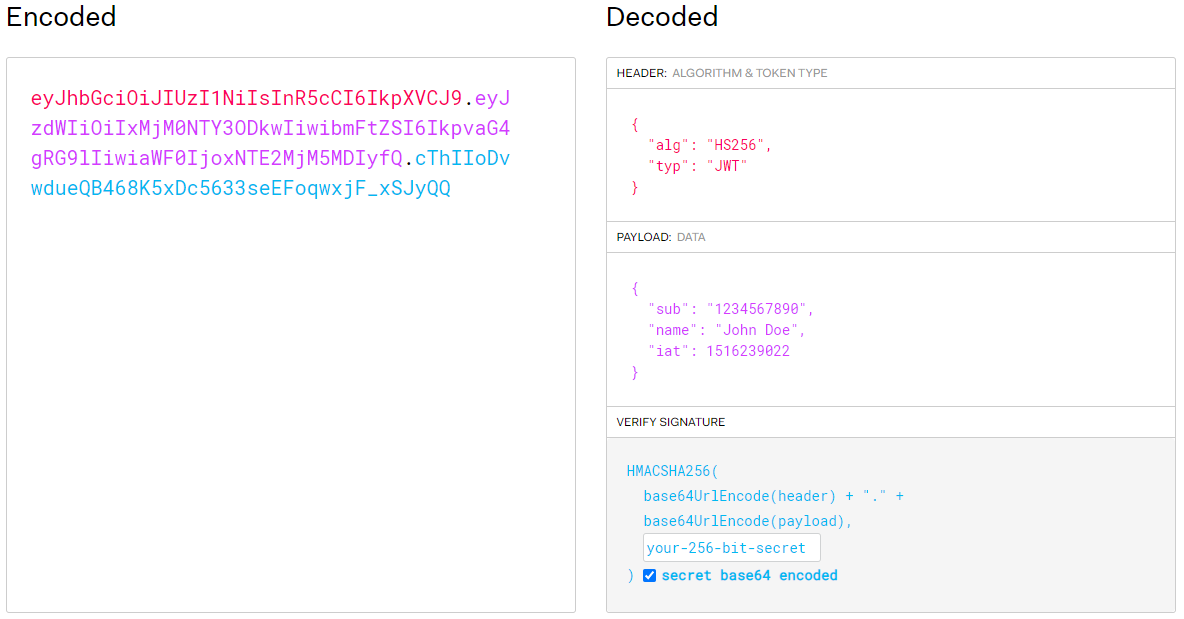
\includegraphics[width=0.85\textwidth]{images/jwt.png}
\caption{Token JWT codificado e descodificado \cite{jwt}}\label{jwt1}
\end{figure}

\subsubsection{Rotas e proteções}

\par Para proteger as páginas apenas referentes a administradores e as gerais ao público não autenticado através da \textit{framework Vue} e da funcionalidade de rotas foram criadas as rotas necessárias para o funcionamento da plataforma e os restantes \textit{end-points} são tratados por uma vista de erro indicando ao utilizador que não existe aquele \textit{end-point}. Em cada rota é aplicado um \textit{middleware} para verificar as permissões. Os \textit{middlewares} criados verificam se o utilizador está autenticado e no caso de serem necessárias permissões se este as possui ou não. Caso o \textit{middleware} indique que não tem acesso a \textit{framework Vue}, redireciona para a rota de tratamento de erro apresentado a mensagem de erro correspondente.

\subsection{Portal Cloud - \textit{Back-end}}

\par O \textit{Back-End} é responsável por fornecer uma API REST ao \textit{Front-end} para o mesmo obter os dados da base de dados. É igualmente responsável por obter os dados provenientes dos \textit{Gateways} das beacons e calcular as suas posições para apresentar no mapa. 
\par O primeiro problema a identificado no \textit{Back-end} é a necessidade de possuir atualizações em tempo real das posições. O \textit{Front-end} não é capaz de calcular quando uma beacon comunica com o \textit{Back-end} apesar da mesma enviar o \textit{broadcast} em tempos regulares, mas tanto a beacon pode não estar ao alcance do \textit{Gateway}, como a mesma pode apenas estar ao alcance de menos de X(dependendo do algoritmo) \textit{Gateways} impossibilitando a utilização do algoritmo. Deste modo não é eficaz o \textit{browser} solicitar ao servidor num intervalo regular qual a posição do elemento no mapa.
\par Para tal além do serviço WEB é disponibilizado um servidor de WEB-Sockets para comunicações em tempo real entre o \textit{Back-end} e o \textit{Front-End}. Os WEB-Sockets é uma tecnologia que permite aos \textit{browsers} mais recentes, ter um canal em tempo real com o \textit{Back-end} sem a necessidade de fazer váris pedidos HTTP, o que acarreta todo o processo do protocolo, como o \textit{3-Way Handshake}. No momento da criação do Web-Socket é criado uma ligação TCP a qual não é finalizada até ao fechar do WEB-Socket, o que elemina o sobre carregamento da criação de pedidos e soluciona o problema da comunicação em tempo real para as atualizações dos mapas.
\par Outro problema e solucionar deparado na análise das tecnologias e soluções existentes é a falta de sincronismo da comunicação dos \textit{Gateways}. Supondo um cenário com 5 \textit{Gateways} e 1 beacon. A beacon ao intervalo de tempo X1 comunica o pacote e apenas 4 \textit{Gateways} recebem o pacote e o enviam para o servidor através de um pedido HTTP. O servidor apesar de ter configurado 5 \textit{Gateways} não é capaz de prever se o 5º \textit{Gateway} irá comunicar a transmissão da beacon, o mesmo pode não estar ao alcance, pode não ter comunicação ao servidor, pode estar desligado ou pode haver algum problema na rede que atrase a chegada do pacote. Igualmente por variados motivos os 4 \textit{Gateways} que enviaram o pacote ao servidor não irão chegar todos em simultaneamente, criando o problema "Já chegaram todos os pacotes? Cálculo com os que tenho, ou espero que chegue mais algum pacote?",
\par O primeiro passo para resolver o problema acima citado ao contrário das soluções mais tradicionais não irá ser utilizado um serviço WEB como o APACHE2 ou o NGINX, pois o mesmo não possui nenhum sincronismo entre pedidos e seria necessário armazenar momentaneamente todos os pacotes na base de dados e ter a tabela em constante escrita e leitura, não sendo o mais eficaz no cenário deste projeto. Para tal o serviço WEB irá ser responsabilidade do NodeJS (módulo express), onde é possível armazenar variáveis entre pedidos distintos que irá ter além do serviço WEB o servidor de WEB-Sockets, centralizando assim os dois serviços e possibilitando igualmente durante o processamento do pedido HTTP o envio de mensagens através do WEB-Socket de forma mais fácil. 
\par Na lista apresentada de seguida estão selecionados os pontos principais das funcionalidades do \textit{Back-End}:

\par
\begin{itemize}
\item API REST para o \textit{Front-End}(Login+ Dados)
\item API REST para o POST dos \textit{Gateways}
\item Serviço WEB (express) para disponibilizar o \textit{Front-End}
\item Serviço WEB-Sockets 
\item Algoritmo de posicionamento
\item Envio de alertas
\end{itemize}
\par

\subsubsection{Sincronismo da rececão de pacotes}
\par Os \textit{Gateways} escolhidos enviam dois tipos de pacotes identificados pelos identificadores GPRP e RSPR. Os pacotes GPRP são referentes ao envio de uma transmissão da beacon. Os pacotes RSPR são referentes ao restante da transmissão da beacon no caso de esta transmitir no Broadcast uma mensagem superior a 31 bytes. O conteúdo do pacote RSPR apenas contem o restante da mensagem não afetando a posição da beacon.
\par De modo ao servidor possuir todos os pacotes GPRP aquando da utilização no momento da chegada este é armazenado numa variável onde é possível consultar as ultimas transmissões de todos os \textit{Gateways}. Quando é recebida uma transmissão do tipo GPRP caso esta seja enviada do \textit{Gateway} X e a ultima transmissão do \textit{Gateway} X for inferior a 5 segundos(intervalo de envio da beacon) este mesmo pacote é descartado, pois o mesmo é referente a um já recebido. Caso seja superior aos 5 segundos do próprio \textit{Gateway} e de todos os restantes, significa que a mesma se trata de uma nova transmissão, neste caso antes de guardar na variável provisória, são selecionados todos os pacotes do intervalo correspondente á ultima transmissão e escolhidos os 4 com o valor mais próximo dos \textit{Gateway}, devido a estes serem os mais fiáveis e é aplicado o algoritmo \textit{Least Squres Estimation} ou simplesmente LSE. Após obtenção da posição estimada esta é guardada na Base de dados para consulta futura e são notificados os clientes de uma nova posição do equipamento. Caso essa posição seja referente a alguma zona de alertas previamente definida é gerado os alertas a enviar. No fluxograma do Apêndice \ref{flux1} é apresentado o fluxograma da aplicação para a receção dos pacotes.


\subsubsection{Diferenças de alturas}

\par Uma questão analisada nos primeiros testes é a divergências nas distâncias observadas quando a beacon apenas se movia no eixo do Z (altura). O \textit{Gateway} calcula a potência do sinal(RSSI) recebido da beacon, esta receção ocorreu em linha reta entre os dois equipamentos e nos mapas utilizados apenas são utilizadas dimensões 2D significando que o valor da distância obtido pelo RSSI é referente ao mesmo em linha reta e não á distancia numa planta 2D, como é apresentado na figura \ref{altura1}.

\begin{figure}[ht]
\centering
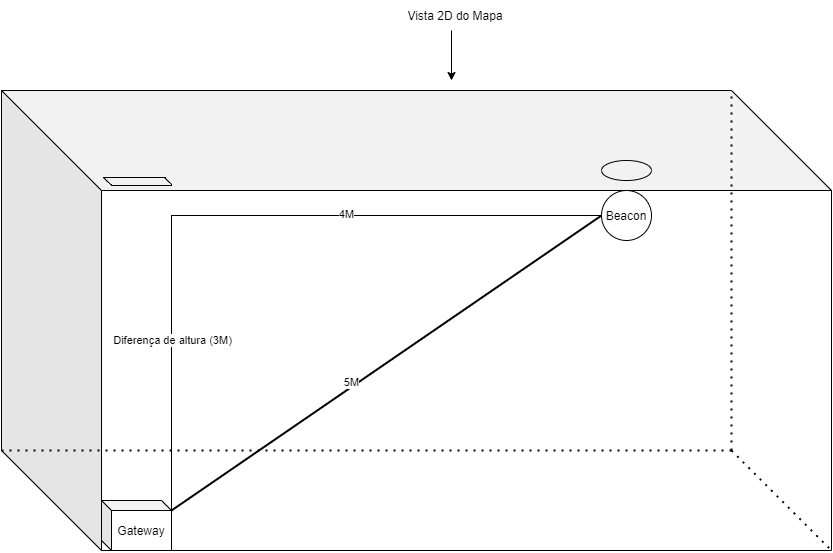
\includegraphics[width=0.95\textwidth]{images/disr.png}
\caption{Diferença entre distâncias Planta vs realidade}\label{altura1}
\end{figure}


\par Para tal na aplicação teve de ser desenvolvido a possibilidade de o utilizador configurar as alturas a que se encontram os \textit{Gateways} e as beacons, de modo a compensar a distância. No exemplo apresentado na figura \ref{altura1} o servidor irá receber a informação que o \textit{Gateway} recebe um pacote com o RSSI correspondente á distância de 5 metros mas no mapa não é a distância a considerar para utilizar o algoritmo que apenas possui suporte a coordenadas 2D. Para tal é necessário conjugar a diferença de alturas e a distância em linha reta para calcular a distância a considerar para o algoritmo, segundo o teorema de Pitágoras. No caso exemplificado ao invés dos 5 metros deve ser considerado os 4 metros.

\subsubsection{Algoritmo de triangulação}

\par Para o projeto foi selecionado o Algoritmo LSE analisado no Capítulo \ref{indoor}, pois o mesmo demonstra os melhores resultados em vários testes. Como parâmetros deste algoritmo é necessário indicar as posições X,Y de cada \textit{Gateway} e a distância calculada previamente segundo o RSSI e o algoritmo de Pitágoras de modo a resolver a diferença referente á altura.
\par No Caso do mapa ter configurado um número superior ao necessário para a utilização do algoritmo, neste caso 4, e nos casos em que existam mais do 4 \textit{Gateways} que receberam comunicações apenas são utilizadas as 4 que tiverem menores valores de distância, isto significa que têm um peso maior no cálculo da posição do mesmo. Previamente á seleção das 4 melhores transmissões caso alguma das transmissões tenha uma distância inferior a 1 metro não é utilizado o algoritmo e é definido a posição da beacon igual á posição do \textit{Gateway} no mapa. Caso não exista nenhum valor abaixo do 1 metro é utilizado o algoritmo indicado. 
\par De modo a otimizar o processamento do algoritmo, devido a este envolver cálculos em matrizes e estas não possuírem tamanhos dinâmicos, não foi utilizado nenhuma biblioteca para realizar as operações em matrizes devido ao sobre carregamento existente nessas bibliotecas. Ao invés os cálculos são realizados manualmente em código segundo as regras de operações das matrizes e o alojamento das suas posições em várias variáveis numéricas. Cada variável possui o valor de uma posição da matriz correspondente. No apêndice \ref{D} é fornecido a função responsável por retornar a posição estimada da beacon ou -1 em caso de erro ou o mapa definido não possua a escala definida, apesar da plataforma não permitir adicionar \textit{Gateways} a mapas sem escala. No caso especifico apresentado nas linhas 47 a 50 de modo a otimizar a velocidade do algoritmo é multiplicado por 0.5 ao invés de 1/2, devido ao fator de para multiplicar o valor por 1/2 ocupa mais tempo do processador, uma vez que são efetuadas duas operações ao invés de apenas uma, uma multiplicação e uma divisão sendo ainda a divisão uma operação mais lenta de efetuar em relação á multiplicação devido a esta ser emulada pelos processadores.

\subsubsection{Filtros - RSSI}

\par Após o desenvolvimento do algoritmo e de alguns testes á receção de pacotes, foi possível analisar numa sala com 6 metros por 6 metros e 4 \textit{Gateways} o sinal das beacons paradas em posições estratégicas o sinal tem algumas flutuações fazendo com que o algoritmo devolva posições incorretas. De modo a eliminar essas flutuações é necessário filtrar os pacotes com ruido e tentar aproximar o valor do esperado. Para tal irá ser utilizado um modelo matemático denominado por Filtro de \textit{Kalman}. Este modelo matemático é capaz de ao longo do tempo consonante os valores recebidos tentar aproximar o valor recebido do espectável segundo a tendência anterior. Deste modo é necessário alterar o servidor de modo a além de guardar temporariamente os pacotes inserir o valor no filtro correspondente. Por cada beacon existente na plataforma existe um conjunto de filtros, um por cada \textit{Gateway} que já recebeu alguma comunicação da beacon. Sempre que um \textit{Gateway} comunicação a receção de um pacote da beacon o valor recebido do RSSI é inserido no filtro onde é retornado o valor estimado segundo os valores anteriormente recebidos. No exemplo da figura \ref{kalman1} é possível observar o funcionamento do filtro ao longo do tempo. Para o projeto é utilizado o plugin JavaScript disponível no GitHub onde é implementado o filtro \textit{Kalman} para dados do tipo 1D. Um dos fatores para a utilização deste filtro ao invés de outros, além da sua utilização por parte de outras pessoas na comunidade científica no âmbito das localizações \textit{inndoor}, foi a necessidade de um algoritmo rápido a estabilizar os dados e que não sobrecarregue o servidor. Após analise do filtro foi possível analisar, que por cada filtro apenas são alojados em memória o último valor e 6 variáveis referente aos cálculos necessários na próxima filtragem, não sendo o espaço assim influenciado pelo tempo que tiver em funcionamento.

\begin{figure}[ht]
\centering
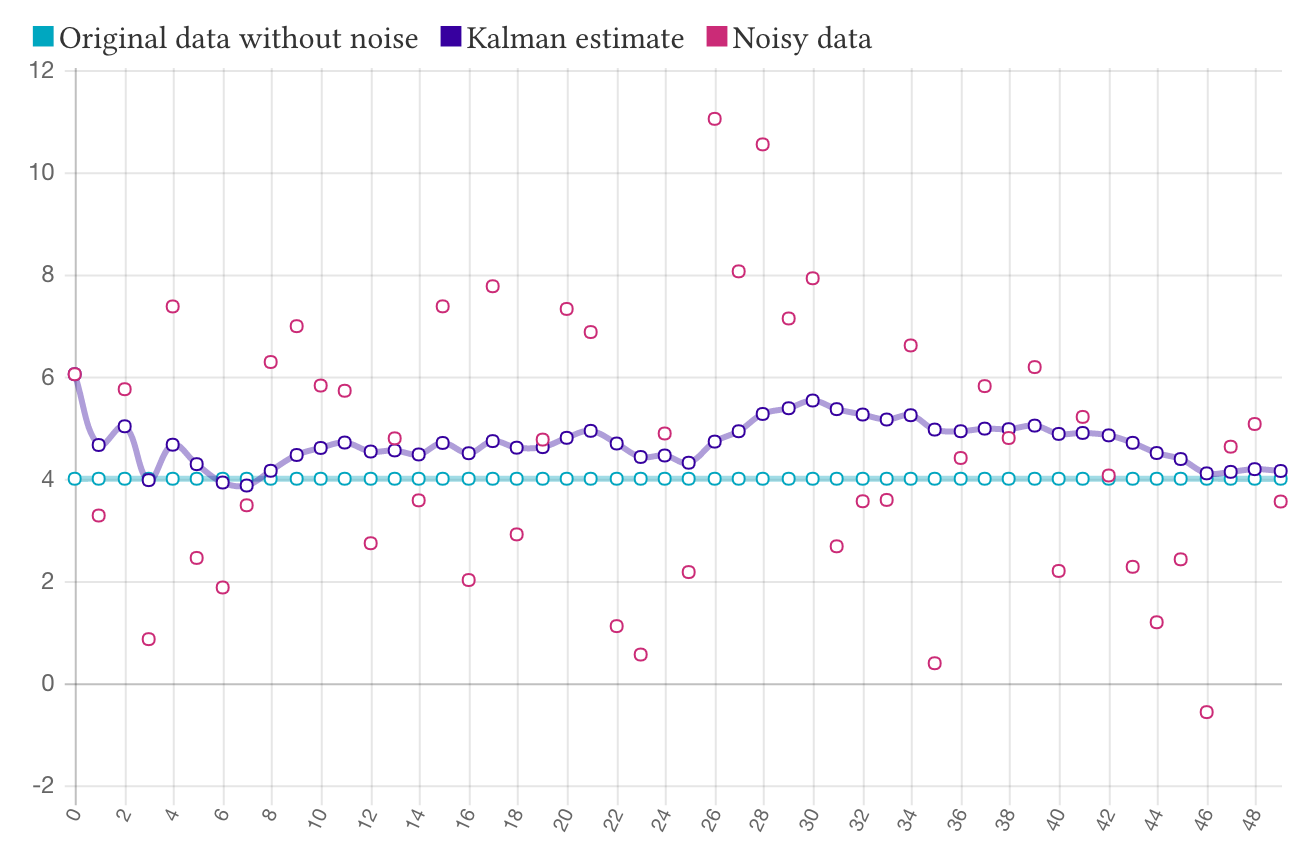
\includegraphics[width=0.90\textwidth]{images/kalman-example.png}
\caption{Exemplo da aplicação do Filtro Kalman \cite{kalman}}\label{kalman1}
\end{figure}



\subsubsection{Filtros - Posição no mapa}

\par Após filtragem do ruido gerado pela transmissão dos dados no meio ambiente, é necessário ainda filtrar certas ocorrências que ocorrem em certas posições e suavizar o movimento quando as beacons se encontram em movimento. O primeiro caso a filtrar referente ao caso da beacon esteja numa posição X1,Y1 no momento t e no momento t+1 em X2,Y2 onde a distância entre pontos é elevada. Para tal quando uma posição é calculada segundo o algoritmo LSE esta posição é comparada com a última guardada do mapa correspondente e é calculada a distância entre ambos os pontos, de seguida é calculada igualmente a velocidade segundo o tempo entre as leituras e a distância. Caso esta seja superior à definida, 5 m/s (18 Km/h), esta posição não é considerada enquanto o tempo entre leituras não permitir o deslocamento da pessoa/objeto para essa mesma posição. O valor máximo da velocidade é possível de ser adaptado consoante o pretendido medir, mas neste caso o cliente pretende monitorar pessoas e objetos. Os objetos alojados no armazém devem ter um deslocamento maioritariamente de 0 pois encontram-se parados e o valor de 5m/s corresponde á possibilidade de estar em movimento num empilhador ou similar. A velocidade média de uma pessoa a andar é de cerca 1 a 2m/s em caminhada\cite{walkingSpeed} e cerca de 1 a 3.8m/s \cite{Long2013}. em corrida, valores sempre inferiores à já definida no intervalo dos objetos.
\par Outro filtro a aplicar é no caso particular de uma beacon se encontrar parada e apesar do filtro \textit{Kalman} filtrar o RSSI a posição possuir pequenas oscilações. Para tal se for gerada uma nova posição, esta passar no filtro da velocidade pois esta se encontra parada e perto da posição da última comunicação com pequenas oscilações e esta oscilação for inferior a 1 metro a posição é guardada para comparação futura mas não é atualizada nos mapas através do Web-Socket. Na próxima receção caso esteja numa posição inferior a 1 metro da posição do mapa dos \textit{browsers} e a menos de 1 metro da ultima posição guardada existente apenas no servidor, não é atualizada a posição apenas novamente no servidor para futura comparação, caso não aconteça e esteja a menos de 1 metro da ultima guardada no servidor e a mais de 1 metro da presente nos \textit{browsers} esta é guardada e enviada para os \textit{browsers} através do Web-Socket. Caso se encontre a uma distância superior a 1 metro em ambas e abaixo dos 5m/s a posição é atualizada no servidor e nos \textit{browsers}.

\subsubsection{Zonas de alerta}

\par Um dos requisitos do cliente na solução é a definição de zonas de alerta, onde é possível indicar se a plataforma deve enviar alertas quando as beacons saem ou entram de uma zona. Para tal além da programação do \textit{Front-end} onde o utilizador através da colocação dos vários vértices da zona indica ao sistema os limites da zona. Após a definição da regra e dos limites é necessário o servidor no cálculo de uma posição verificar se a beacon saiu ou entrou numa zona definida como alarme. No caso de polígonos regulares tais como círculos, retângulos, triângulos é facilmente calculado se um ponto se encontra dentro da área. No caso de polígonos irregulares o caso é diferente. Para tal foi utilizado na solução o plugin "point-in-polygon" \cite {pointpoint}. Este algoritmo é capaz de indicar se um determinado ponto X,Y se encontra dentro do polígono ou fora, definido pelos conjunto de pontos fornecidos .

\subsection{Reutilização de beacons}

\par De modo a contruir uma plataforma modular e reutilizável cada beacon pode ser reutilizada na plataforma. No momento da configuração é adicionada uma beacon á conta da \textit{Company}. Para as posições serem guardadas na base de dados é necessário o utilizador aceder á plataforma e iniciar uma missão indicando a data de início e se pretende localizar pessoas ou objetos e qual o utilizador/ objeto a localizar. Neste momento sempre que a beacon seja localizada nos mapas referentes á \textit{Company} detentora da beacon a posição é guardada com informação sobre a missão do \textit{tracking}. Quando a beacon já não é necessária o utilizador pode terminar a missão da beacon e a plataforma deixa de registar as posições enquanto não possuir missão ativa novamente. Desta forma o cliente pode adquirir várias beacons, mas caso pretenda mudar de objetivo, como por exemplo um empregado deixe de trabalhar na empresa e começar outro funcionário pode ser trespassada a beacon e nos históricos estes ficam separados e é possível de forma intuitiva decidir quais os dados que são de cada utilizador, excluindo a necessidade de utilizar uma beacon com um identificador diferente (MAC) para isso.
\par


\chapter{Testes e Avaliação}\label{cap4}
\par Neste capítulo irá ser abordado os testes e a avaliação do trabalho desenvolvido durante o estágio e apresentado no capítulo \ref{workcharp}. À semelhança dos capítulos anteriores, o capítulo está divido em vários, um por cada projecto. Todos os projetos obtiveram resultados positivos em relação aos objetivos abordados no início do estágio.

\section{Nidus}

\par Durante os desenvolvimentos ocorridos durante a realização do estágio foram testados as novas funcionalidades desenvolvidas, nomeadamente em relação à compressão dos ficheiros e das imagens. 
\par A compressão das imagens e utilização dos SVG ao invés dos PNG e JPEG, como foi indicado no subcapítulo \ref{custom}, foi implementada com sucesso e abriu novas possibilidades  no sistema Nidus epermitiu igualmente para o seu utilizador uma melhor fluidez nas animações e nas transições.
\par A compressão dos ficheiros com recurso à mudança do método de compressão originalmente o GZIP para Brotli obteve bons resultados, como indicado na tabela \ref{tabw2}, nos ficheiros atuais da Nidus e permitiu libertar espaço suficiente para alocar as restantes funcionalidades desenvolvidas no estágio tais como o sistema de internacionalização. ou a adaptação futura do plugin Blockly na gestão de eventos.

\section{Nb-Iot}

\par Os testes realizados no \textit{firmware} desenvolvido demonstraram a capacidade de este utilizar toda a memória disponível sem ocorrerem necessidade de alocar memória e não existir disponível. Comparada mente com o \textit{firmware} inicial, o qual não permitia algumas funcionalidades tais como o envio para o portal das suas configurações e apenas o envio das leituras e com um limite de 25 leituras de Log, o \textit{firmware} desenvolvido possui todas as necessidades do projeto tais como a comunicação bidirecional entre o portal. No \textit{Firmware} desenvolvido e o equipamento obteve nos testes realizados um limite de 170 Logs com o valor máximo de sensores estipulados(6) o qual pode ser configurado e caso este seja alterado a possibilidades de aumentar a capacidade de Log é possível. Para um máximo de 3 sensores o valor máximo de leituras em Log sobe para 340 e sobe para 1020 no caso de apenas ser alocado o espaço para um sensor.

\section{Kea Tracker}

\par Neste projeto o desenvolvimento limitou-se apenas à aplicação visto durante a realização dos restantes projetos ter sido fornecido uma versão já com suporte às funcionalidades requeridas. Focou-se assim o projeto no desenvolvimento da aplicação multiplataforma a qual integrou todas as funcionalidades já existentes com sucesso e a inclusão das novas funcionalidades  referentes ao \textit{download} dos Logs e ao sincronismo de leituras que permite ao utilizador final uma precisão garantida ao minuto.

\section{dot.tracker}

\par A plataforma dot.Tracker durante os testes demonstrou-se cerca de 5 a 6 vezes mais rápida relativamente ao protótipo desenvolvido com recurso à \textit{Framework} Laravel, além de corrigir os problemas identificados e apresentados ao longo deste relatório. Os filtros desenvolvidos/ aplicados conseguem com sucesso atenuar as oscilações presentes nas comunicações, garantindo um movimento mais estável e mais suave. 
\par  A adoção da correção de altura demonstrou ser uma importante fase no cálculo da posição estimada do equipamento. Durante estes testes foi possível constatar, um problema na utilização do método atual para cálculo da distância visto que no caso de ser configurada uma altura na plataforma e o equipamento se mover no eixo Z correspondente à altura os resultados obtidos aumentam o erro consoante a diferença de altura real e a calculada.  Ainda referente à altura no caso de oscilações muito grandes  e em casos específicos o algoritmo descarta pacotes visto não terem sentido. Supondo o teste realizado com um \textit{beacon} e alguns recetores. Configurando na plataforma a altura do \textit{beacon} a 10 M de altura e a altura do recetor a 0 M de altura, caso seja rececionado com um pacote com o RSSI correspondente a uma altura  perto de 10 M é possível  obter a distância a colocar no mapa como elucidado na figura \ref{altura1}. Caso seja movido o \textit{beacon} para uma altura de por exemplo 0.5 M o algoritmo desenvolvido ao compensar a distância com a diferença de alturas não é capaz de calcular esse valor visto que segundo o algoritmo de Pitágoras não é possivel obter um triângulo retângulo com um cateto de 10 M e a hipotenusa de 0.5 M. Nestes casos a plataforma não calcula  a sua posição no mapa.
\par A respeito da precisão do sistema em geral é possível obter uma precisão média entre 1 a 2 metros  consoantes os ambientes, o seu conteúdo ou simplesmente às interferências existentes. De modo a aumentar a  precisão em ambientes mais hostis para localização o aumento do número de recetores e menor distância entre eles permite melhores resultados.

\clearpage \cleardoublepage %!!!!!!!!!!!!!!!!!!!!!!!!!!!!!!!!!!!!!!!!!!!!!!!!!!!!!!!!!!!!!!!!!!!!!!!!!!!!!!!!!!!!!!!!!!!!!!!!!!


\chapter{Conclusões e Trabalho Futuro}
\par Inserido num contexto empresarial , e tratando-se de projetos em desenvolvimento e de desenvolvimento contínuo, estes não foram concluidos com o concluir deste relatório e estágio. Todos os objetivos defindos no inicio do estágio foram concluidos com sucesso e com bons resultados como apresentado no capítulo \ref{cap4}. 
\par A realização de um estágio com projetos reais em ambiente empresarial permitiu uma melhor compreensão dos vários fatores que  não são possiveis replicar em ambiente académico, além da utilizaão de novas metodologias e técnologias.

\par Para trabalho futuro prevê-se a implementação do plugin Blockly na página da Nidus, algumas alterações simples de Design na página e a reformulação da ferramenta de compressão da página para a utilização do Brotli.
O projeto do Nb-Iot caso exista atualizações de \textit{Firmware} por parte da Digi que permitam a comunicação por Bluetooth, será implementada a configuração do equipamento através de uma aplicação móvel. No projeto dot.Tracker caso a necessidade de aumentar a precisão se venha a verificar, deve-se ponderar a migração para um sistema diferente de localização indoor sem recurso ao valor de RSSI tal como o \textit{Bluetooth} 5.1, em desenvolvimento, especialmente desenhado para localização em ambientes fechados. O \textit{Bluetooth} 5.1 com recurso a várias antenas por recetor, consegue calcular o ângulo entre o emissor e o recetor e com recurso a vários recetores delimitar a posição do emissor.

\par A utilização de \textit{Frameworks} que permitam o desenvolvimento de aplicações multiplataforma, tais como a utilizada neste estágio, o IONIC, é uma mais valia, pois utilizando o mesmo código fonte desenvolvido, permite além de manter o Design similar entre as plataformas, diminui o tempo de desenvolvimento quando são necessárias correções e atualizações e caso não seja necessário pelos requiesitos da aplicação, abstrai o desenvolvimento da programação nativa em cada ambiente, para \textit{Frameworks} de mais alto nível.

\par O estágio na Captemp foi uma experiência enriquecedora, onde foi possivel obter e consolidar conhecimento já adquiridos e novos, experiência e criadas novas relações quer a nível profissional quer pessoal.

% REFERENCES
% Edit the references.bib file to add your own references, that you can then
% \cite on your text.

\clearpage \cleardoublepage %!!!!!!!!!!!!!!!!!!!!!!!!!!!!!!!!!!!!!!!!!!!!!!!!!!!!!!!!!!!!!!!!!!!!!!!!!!!!!!!!!!!!!!!!!!!!!!!!!!



\bibliographystyle{ieeetr}

\addcontentsline{toc}{chapter}{Bibliografia}
\bibliography{references}

\clearpage \cleardoublepage %!!!!!!!!!!!!!!!!!!!!!!!!!!!!!!!!!!!!!!!!!!!!!!!!!!!!!!!!!!!!!!!!!!!!!!!!!!!!!!!!!!!!!!!!!!!!!!!!!!


\clearpage %\cleardoublepage %for openright
\renewcommand{\thesection}{Apêndices \Roman{section}}

\begin{appendices}

\clearpage \cleardoublepage

\chapter{Exemplo de um SVG} \label{svg}
\begin{lstlisting}[caption=Exemplo de um SVG,label={xml4},language=XML]

<?xml version="1.0" encoding="UTF-8" standalone="no"?>
<!-- Created with Inkscape (http://www.inkscape.org/) -->
<svg
	xmlns:dc="http://purl.org/dc/elements/1.1/"
	xmlns:cc="http://creativecommons.org/ns#"
	xmlns:rdf="http://www.w3.org/1999/02/22-rdf-syntax-ns#"
	xmlns:svg="http://www.w3.org/2000/svg"
	xmlns="http://www.w3.org/2000/svg"
	xmlns:sodipodi="http://sodipodi.sourceforge.net/DTD/sodipodi-0.dtd"
	xmlns:inkscape="http://www.inkscape.org/namespaces/inkscape"
   width="10mm"
   height="10mm"
   viewBox="0 0 10 10"
   version="1.1"
   id="svg8"
   inkscape:version="0.92.5 (2060ec1f9f, 2020-04-08)"
   sodipodi:docname="desenho1.svg">
	<defs
     id="defs2" />
	<sodipodi:namedview
     id="base"
     pagecolor="#ffffff"
     bordercolor="#666666"
     borderopacity="1.0"
     inkscape:pageopacity="0.0"
     inkscape:pageshadow="2"
     inkscape:zoom="15.839192"
     inkscape:cx="56.676533"
     inkscape:cy="22.492236"
     inkscape:document-units="mm"
     inkscape:current-layer="layer1"
     showgrid="false"
     inkscape:window-width="1920"
     inkscape:window-height="1017"
     inkscape:window-x="-8"
     inkscape:window-y="-8"
     inkscape:window-maximized="1" />
	<metadata
     id="metadata5">
		<rdf:RDF>
			<cc:Work
         rdf:about="">
				<dc:format>image/svg+xml</dc:format>
				<dc:type
           rdf:resource="http://purl.org/dc/dcmitype/StillImage" />
				<dc:title></dc:title>
			</cc:Work>
		</rdf:RDF>
	</metadata>
	<g
     inkscape:label="Layer 1"
     inkscape:groupmode="layer"
     id="layer1"
     transform="translate(0,-287)">
		<rect
       style="fill:#ff0000;stroke-width:0.26458332"
       id="rect10"
       width="9.1205721"
       height="4.660512"
       x="0.3674956"
       y="287.3783" />
		<circle
       style="fill:#00ffff;stroke-width:0.26458332"
       id="path12"
       cx="3.5747297"
       cy="293.07449"
       r="2.3887215" />
		<text
       xml:space="preserve"
       style="font-style:normal;font-weight:normal;font-size:1.2726717px;line-height:1.25;font-family:sans-serif;letter-spacing:0px;word-spacing:0px;fill:#000000;fill-opacity:1;stroke:none;stroke-width:0.03181679"
       x="8.6893291"
       y="242.43219"
       id="text18"
       transform="scale(0.82155341,1.2172063)">
			<tspan
         sodipodi:role="line"
         id="tspan16"
         x="8.6893291"
         y="242.43219"
         style="stroke-width:0.03181679">SVG </tspan>
		</text>
	</g>
</svg>


\end{lstlisting}

\clearpage \cleardoublepage

 \chapter{Exemplo de um SVG comprimido} \label{svggo}
\begin{verbatim}

<svg xmlns="http://www.w3.org/2000/svg" width="10mm" height="10mm" 
viewBox="0 0 10 10">
    <g transform="translate(0 -287)">
        <path fill="red" d="M.367 287.378h9.121v4.661H.367z" />
        <circle cx="3.575" cy="293.074" r="2.389" fill="#0ff" />
        <text style="line-height:1.25" x="8.689" y="242.432" 
transform="scale(.82155 1.2172)" font-weight="400" font-size="1.273" 
font-family="sans-serif" letter-spacing="0" word-spacing="0" 
stroke-width=".032">
            <tspan x="8.689" y="242.432">SVG</tspan>
        </text>
    </g>
</svg>


\end{verbatim}

\clearpage \cleardoublepage
\chapter{Fluxograma dos processos de Registo -App}\label{E}
 \begin{figure}[htb]
\centering
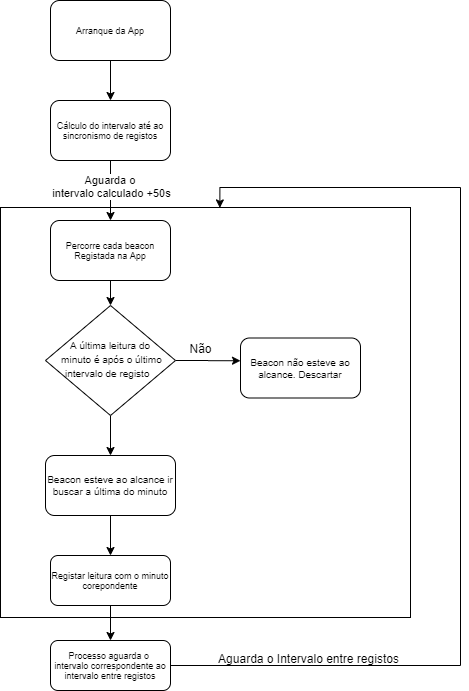
\includegraphics[width=0.79\textwidth]{images/flux2.png}
%\caption{Fluxograma do processo de receção de pacotes}\label{flux1}
\end{figure}


\clearpage \cleardoublepage

\chapter{Fluxograma do processo de Envio - App}\label{F}
 \begin{figure}[htb]
\centering
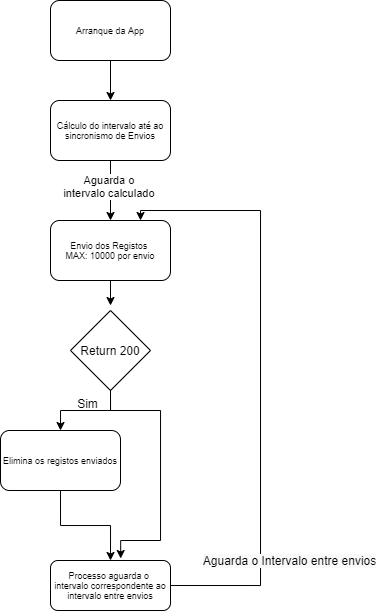
\includegraphics[width=0.50\textwidth]{images/flux20.png}
%\caption{Fluxograma do processo de Envio}






\end{figure}

\clearpage \cleardoublepage

\chapter{Fluxograma de receção de Pacotes BLE}\label{G}
 \begin{figure}[htb]

\centering
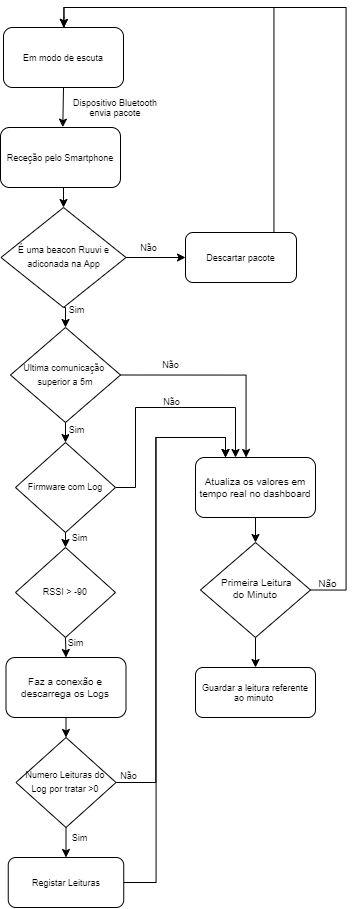
\includegraphics[width=0.45\textwidth]{images/flux21.png}
%\caption{Fluxograma do processo de receção de Pacotes BLE}






\end{figure}


\clearpage \cleardoublepage
 \chapter{Fluxograma do processo de receção de pacotes} \label{flux1}
 \begin{figure}[htb]
\centering
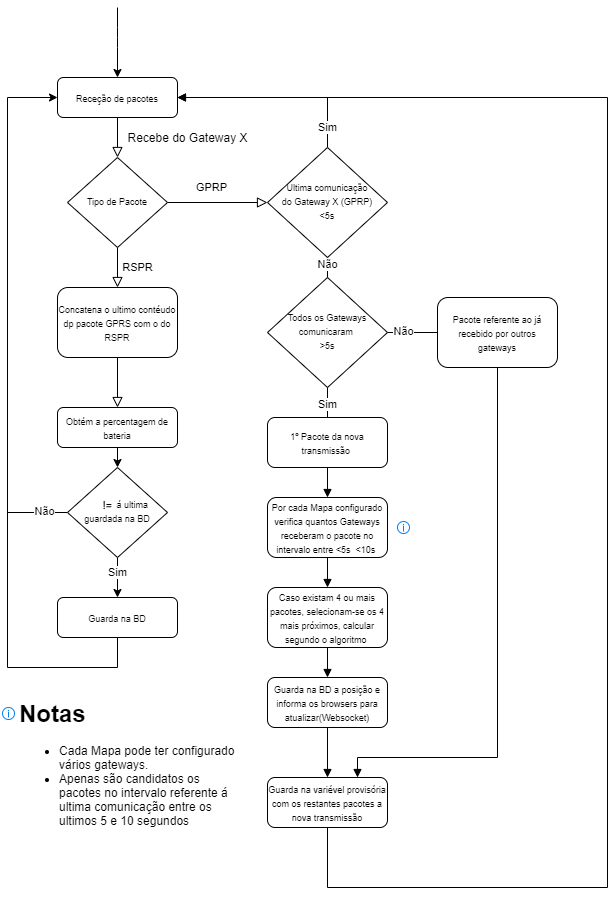
\includegraphics[width=0.79\textwidth]{images/flux1.png}
%\caption{Fluxograma do processo de receção de pacotes}\label{flux1}
\end{figure}

\clearpage \cleardoublepage
\chapter{Código da obtenção da posição - LSE}\label{D}
\begin{verbatim}
1  function getPosLSE(d1,d2,d3,d4,n1,n2,n3,n4,scale){
2      if(scale==null){
3          return -1;
4      }
5
6      /*Convert values from String to Float*/
7      scale=parseFloat(scale);
8      d1=parseFloat(d1);
9      d2=parseFloat(d2);
10     d3=parseFloat(d3);
11     d4=parseFloat(d4);
10
11     /*matriz A
12     | a  d |
13     | b  e |
14     | c  f |
15     */
16     var a=(n2.x)-(n1.x);
17     var b=(n3.x)-(n1.x);
18     var c=(n4.x)-(n1.x);
19     var d=(n2.y)-(n1.y);
20     var e=(n3.y)-(n1.y);
21     var f=(n4.y)-(n1.y);
22
23     /*transposta de A
24     | a b c |
25     | d e f |
26     
27     At * a
28     | aa bb |
29     | cc dd |
30     */
31
21     var aa=(a*a)+(b*b)+(c*c);
22     var bb=(a*d)+(b*e)+(c*f);
23     var cc=bb; /*(d*a)+(e*b)+(f*c);*/
24     var dd=(d*d)+(e*e)+(f*f);
25
26     /*determinante de At*A
27
28     var det=(aa*dd)-(bb*cc);
29     if(det!=0)
30         {
31             /*pode proceguir há inversa
32
33             inversa
34             | aaa  bbb |
35             | ccc  ddd |
36
37             formula
38             | dd/det  -bb/det | 
39             | -cc/det  aa/det |
40             */
41             var aaa=dd/det;
42             var bbb=-(bb/det);
43             var ccc=-(cc/det);
44             var ddd=(aa/det);
45
46             /* Multiplicar por 1/2
47             var aaaa=aaa*0.5;
48             var bbbb=bbb*0.5;
49             var cccc=ccc*0.5;
50             var dddd=ddd*0.5;	
51
52             /* multiplicar pela transposta
53                 | aaaa bbbb |   *  | a b c |
54                 | cccc dddd |      | d e f |
55             */
56             var a5=(aaaa*a)+(bbbb*d);
57             var b5=(aaaa*b)+(bbbb*e);
58             var c5=(aaaa*c)+(bbbb*f);
59             var d5=(cccc*a)+(dddd*d);
60             var e5=(cccc*b)+(dddd*e);
61             var f5=(cccc*c)+(dddd*f);
62
63             /* definir b
64            | b1 |
65            | b2 |
66            | b3 |
67
68             var d12=Math.pow((d1*scale),2);
69             var b1=Math.pow((n2.x),2) - Math.pow((n1.x),2)
+ Math.pow((n2.y),2) - Math.pow((n1.y),2) - Math.pow((d2*scale),2) + d12;
70             var b2=Math.pow((n3.x),2) - Math.pow((n1.x),2)
+ Math.pow((n3.y),2) - Math.pow((n1.y),2) - Math.pow((d3*scale),2) + d12;
71             var b3=Math.pow((n4.x),2) - Math.pow((n1.x),2)
+ Math.pow((n4.y),2) - Math.pow((n1.y),2) - Math.pow((d4*scale),2) + d12;
72 
73
74             /* Multiplicar por b
75             | a5 b5 c5 |       *        | b1 |
76             | d5 e5 f5 |                | b2 |
77                                         | b3 |
78             */
79             var resX=(a5*b1)+(b5*b2)+(c5*b3);
80             var resY=(d5*b1)+(e5*b2)+(f5*b3);
81             return {"x":resX,"y":resY};
82         }
83         return -1;
84  }
\end{verbatim}



\end{appendices}

\end{document}
